\section{Verifiche del cinematismo}
Si procede ora con la verifica degli elementi del cinematismo.
\subsection{Spinotto}
Il primo componente sottoposto ad analisi è lo spinotto, le cui caratteristiche geometriche e di carico risultano espresse in Fig.\ref{fig:CarichiSpinotto}.\\
\begin{figure}[h]
\centering
   {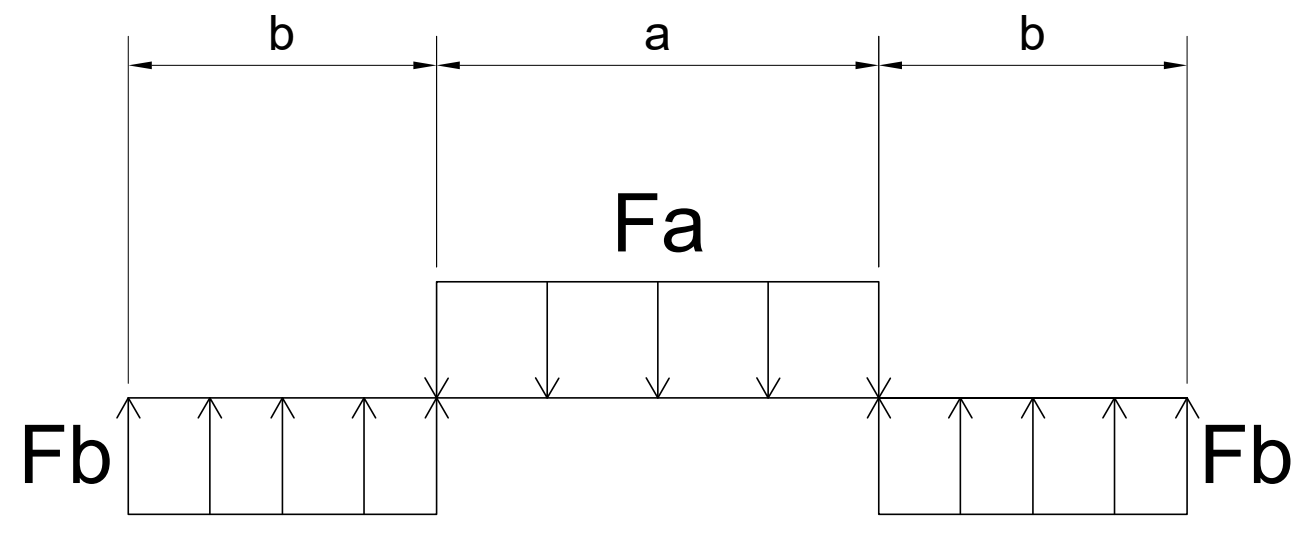
\includegraphics[width=.48\textwidth]{Immagini/CarichiSpinotto1.png}} \quad
   {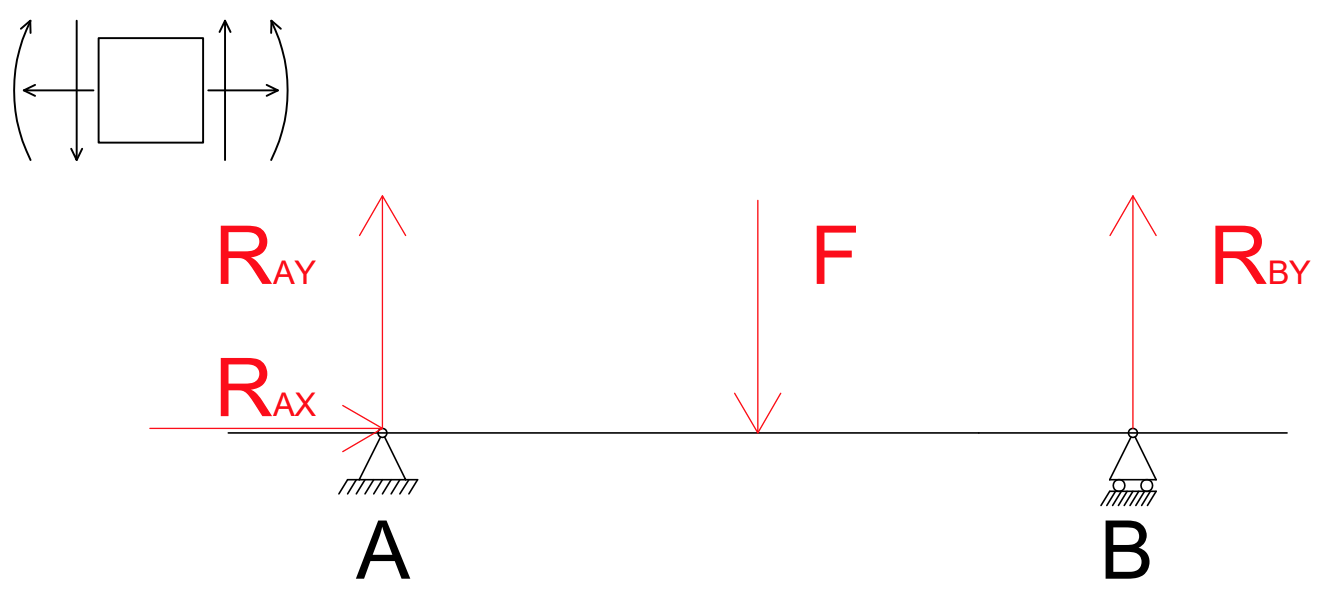
\includegraphics[width=.48\textwidth]{Immagini/CarichiSpinotto2.png}}
\caption{Schematizzazione sollecitazione spinotto}
\label{fig:CarichiSpinotto}
\end{figure}
\\
dove:
\begin{itemize}
    \item $a=19\ mm$
    \item $b=13,25\ mm$
    \item $F_a=2500\ N$
    \item $F_b=\frac{Fa}{2}=1250\ N$
\end{itemize}
avendo assunto una distribuzione delle pressioni di contatto sullo spinotto costante lungo l'asse del componente.\\
\\
Attraverso uno studio di Scienza delle Costruzioni, basato su una schematizzazione a trave, si ottengono i seguenti diagrammi di caratteristiche delle sollecitazioni.
\begin{figure}[h]
    \centering
    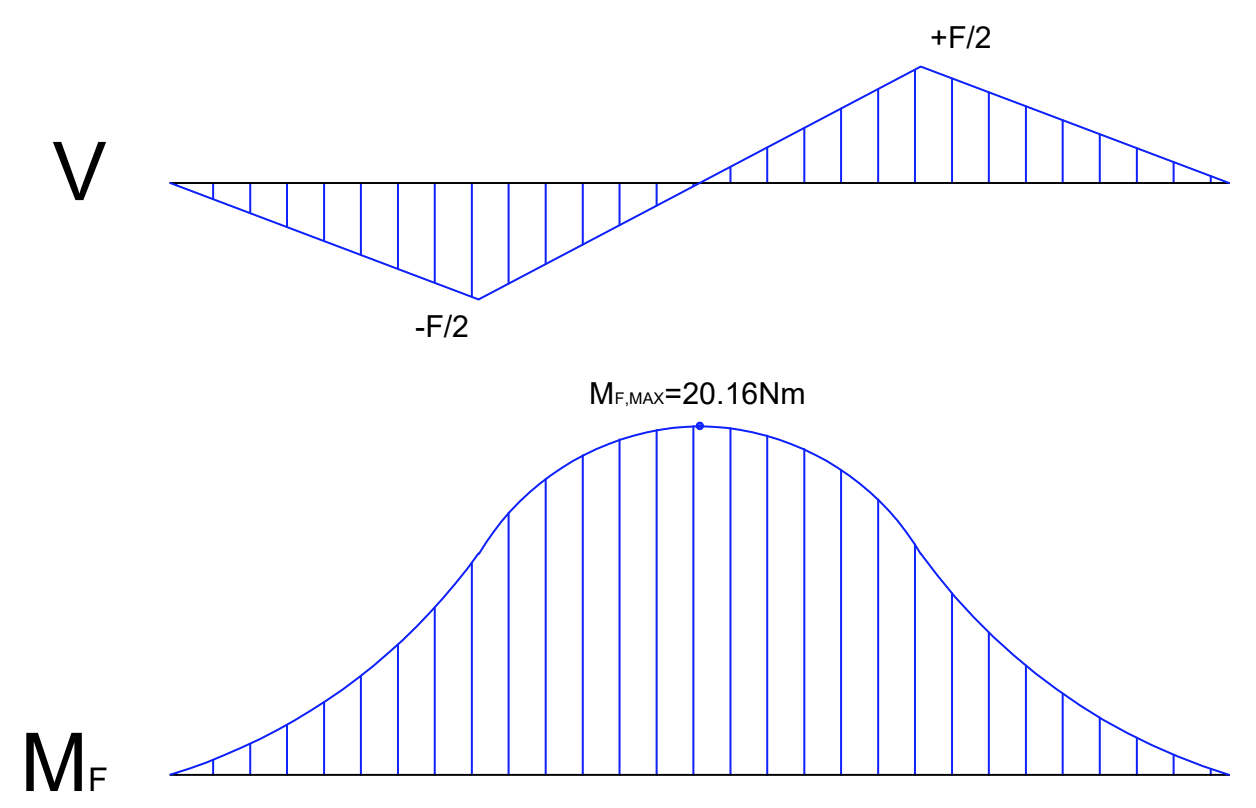
\includegraphics[scale=0.4]{Immagini/SollecitazioniSpinotto.png}
    \caption{Andamento delle sollecitazioni lungo lo spinotto}
    \label{fig:SollecitazioniSpinotto}
\end{figure}
\newpage
Durante il funzionamento del cinematismo, lo spinotto è sottoposto a diverse tipologie di carico:
\begin{itemize}
    \item taglio puro
    \item flessione
    \item ovalizzazione
\end{itemize}
\subsubsection{Taglio puro} 
Dall'analisi a taglio della Fig.\ref{fig:SollecitazioniSpinotto} si deduce che le sezioni maggiormente interessate da questo tipo di sforzo saranno in corrispondenza dei picchi del diagramma (sezioni 2, Fig.\ref{fig:SezioniCriticheSpinotto}).\\
Si calcola attraverso la seguente formula la massima tensione tangenziale $\tau$ in corrispondenza dell'asse passante per i punti C e C' di Fig.\ref{fig:TaglioSezioneSpinotto2}.
\begin{equation}
    \tau=\frac{4}{3}\frac{F_a}{\frac{\pi}{2}\left(D^2-d^2\right)}=24,11\ MPa
\end{equation}
con $D=13\ mm$ e $d=8,4\ mm$.
\begin{figure}[h]
    \centering
    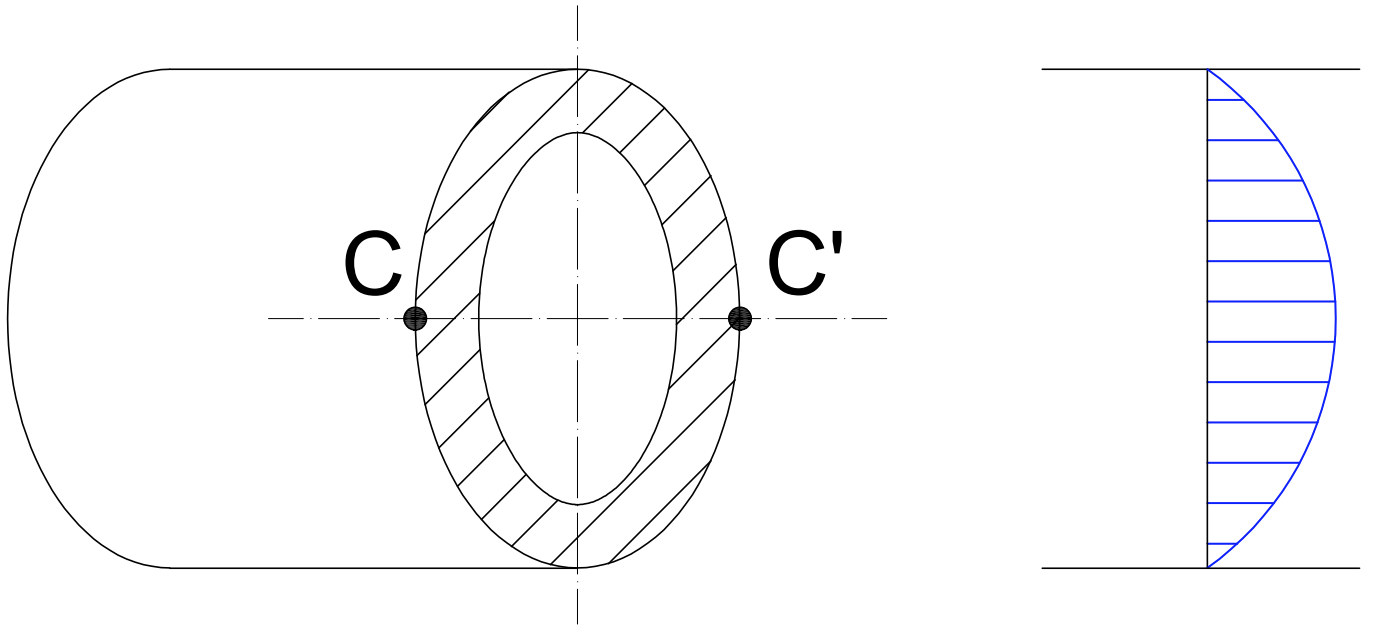
\includegraphics[scale=0.4]{Immagini/TaglioSezionesSpinotto2.png}
    \caption{Andameto delle tensioni di taglio lungo le sezioni 2}
    \label{fig:TaglioSezioneSpinotto2}
\end{figure}
\subsubsection{Flessione}
Seguendo l'approccio già utilizzato, si procede alla valutazione degli sforzi dovuti alla sollecitazione di flessione. \\
Analogamente a quanto fatto in precedenza, osservando Fig.\ref{fig:SollecitazioniSpinotto} si nota che la sezione maggiormente sollecitata da questo tipo di sforzo, risulterà essere quella di mezzeria in corrispondenza del momento flettente massimo.\\
Si può valutare l'entità dello sforzo massimo $\sigma_f$ sulla sezione 1 (sezione sollecitata a massimo momento flettente), in corrispondenza dei punti A ed A', attraverso la seguente formula:
\begin{equation}
    \sigma_f=\frac{M_{f,Max}}{W}=113,20\ MPa
\end{equation}
dove $W=\frac{\pi\left(D^4-d^4\right)}{32D}=178,09\ mm^3$.
\newpage
\begin{figure}[h]
    \centering
    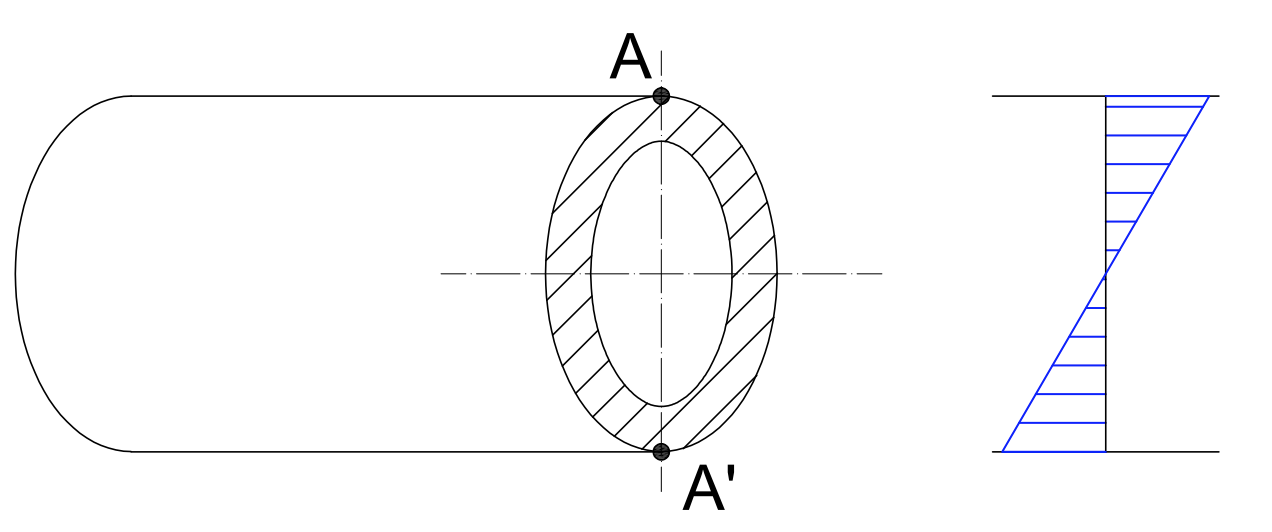
\includegraphics[scale=0.5]{Immagini/FlessioneSezioneSpinotto1.png}
    \caption{Andamento delle tensioni di flessione lungo la sezione 1}
    \label{fig:FlessioneSezioneSpinotto1}
\end{figure}
\subsubsection{Ovalizzazione} 
Questo tipo di stato tensionale non deriva dalla schematizzazione a trave precedentemente discussa, ma si manifesta nel caso in cui le forze in gioco siano molto elevate e lo spinotto sia di ridotte dimensioni. 
La tensione di ovalizzazione si calcola con la seguente formula:
\begin{equation}
    \sigma_o=\frac{3}{4}\frac{F_a\cdot r_m}{l\cdot s^2}=41,68\ MPa
\end{equation}
dove $r_m=\frac{r_e+r_i}{2}=5,35\ mm$ è il raggio medio, $l=45,5\ mm$ è la lunghezza dello spinotto e $s=2,3\ mm$ il suo spessore.
\begin{figure}[h]
    \centering
    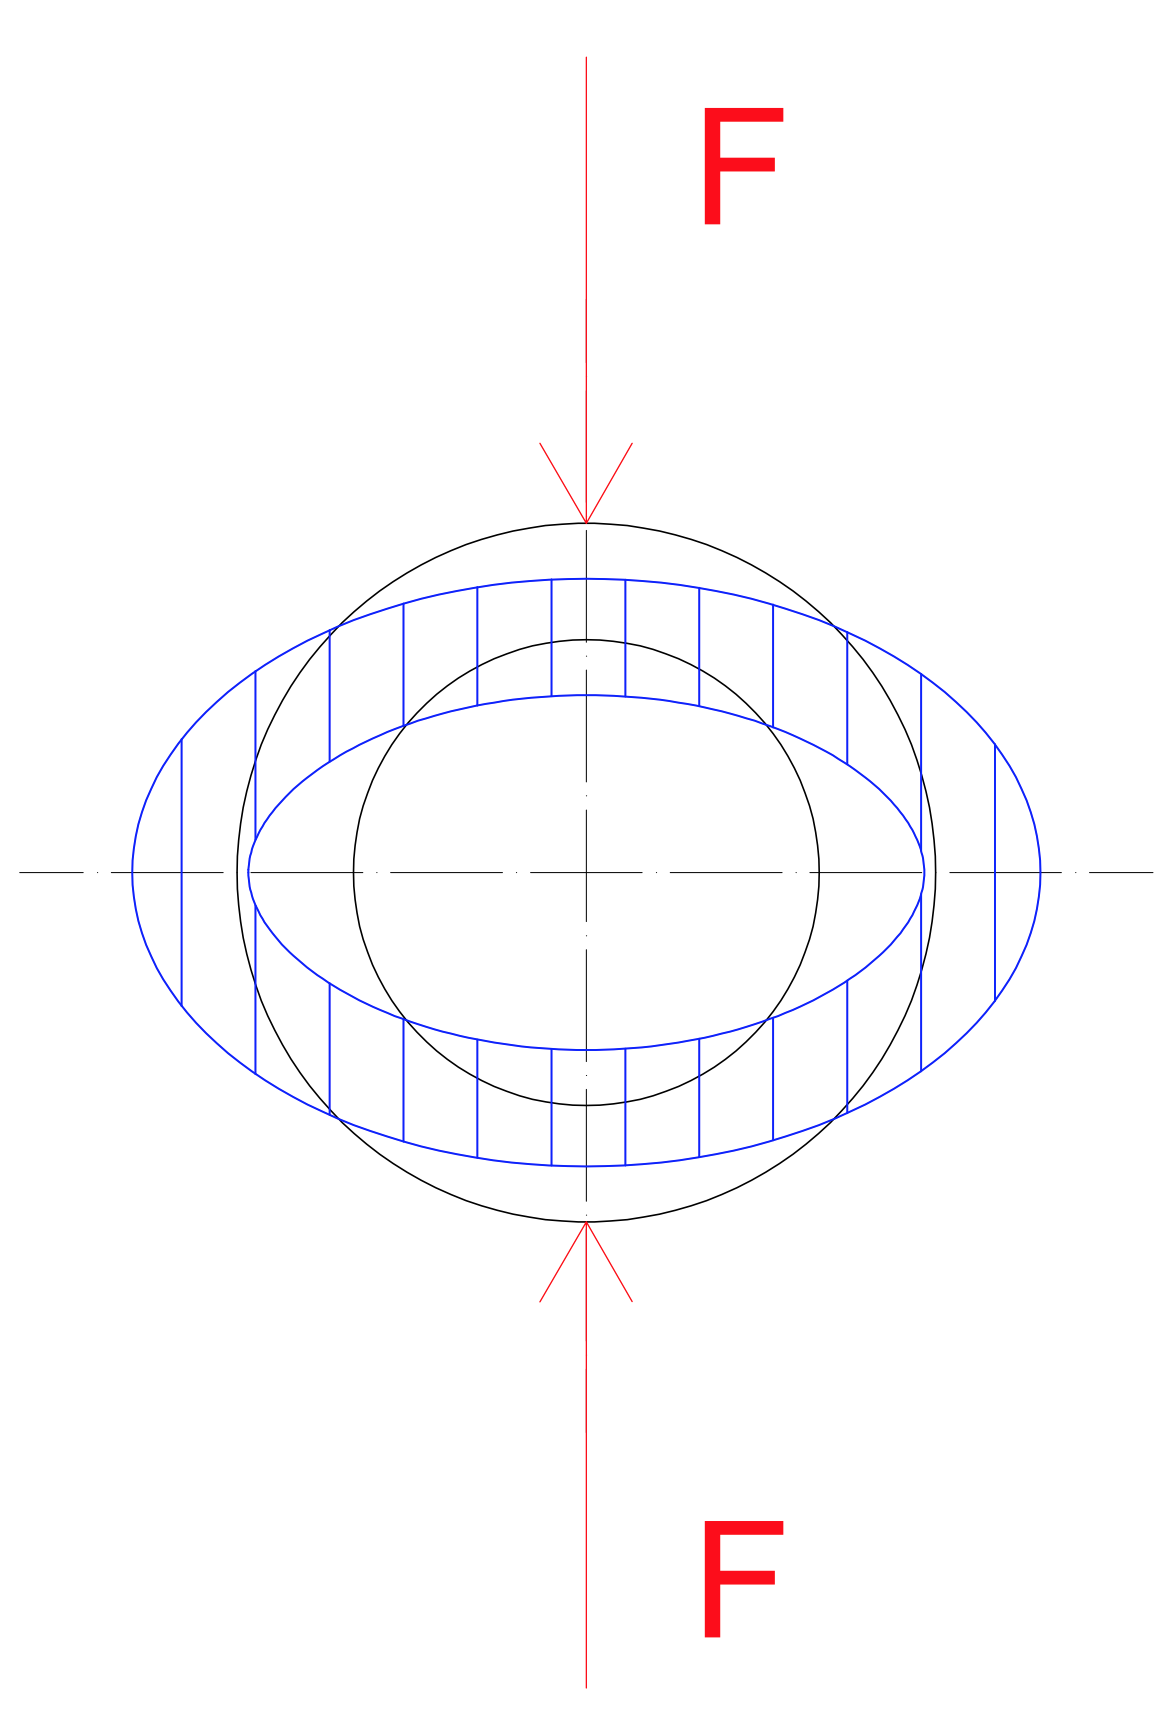
\includegraphics[scale=0.3]{Immagini/OvalizzazioneSezioneSpinotto.png}
    \caption{Rappresentazione deformata di ovalizzazione}
    \label{fig:OvalizzazioneSezioneSpinotto}
\end{figure}
\newpage
\subsubsection{Verifica Statica}
Da quanto osservato fin ora, le sezioni maggiormente sollecitate risultano essere:
\begin{itemize}
    \item sezione 1, in corrispondenza della mezzeria del componente
    \item sezione 2, a distanza b dall'estremità dello spinotto 
\end{itemize}
\begin{figure}[h]
    \centering
    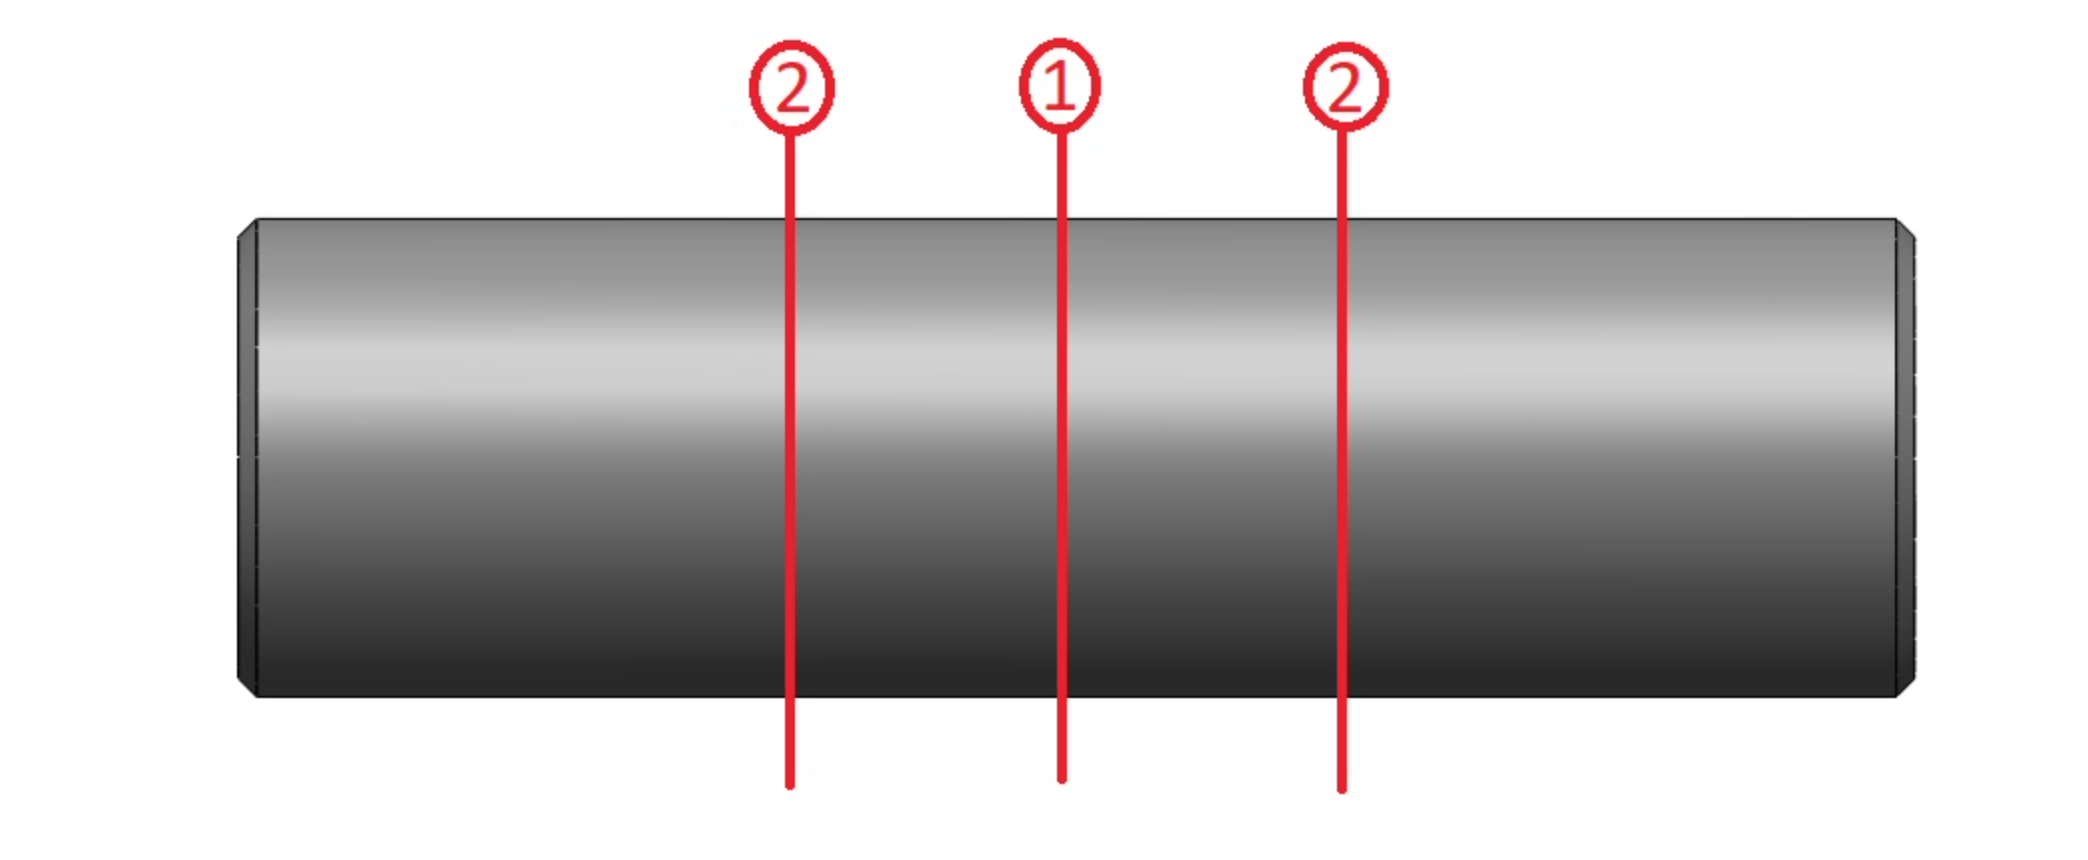
\includegraphics[scale=0.3]{Immagini/SezioniCriticheSpinotto.png}
    \caption{Posizione delle sezioni critiche per lo spinotto}
    \label{fig:SezioniCriticheSpinotto}
\end{figure}
\paragraph{Sezione 1} Nella prima sezione sono presenti sollecitazioni di flessione ed ovalizzazione, mentre il taglio risulta essere nullo (Fig.\ref{fig:SollecitazioniSpinotto}).\\
Combinando i due andamenti noti delle sollecitazioni appena definite, si ottiene una configurazione rappresentata in Fig.\ref{fig:Sezione1Spinotto}, dove è possibile osservare che in corrispondenza del punto A è presente lo stato di massimo sforzo.\\
\begin{figure}[h]
    \centering
    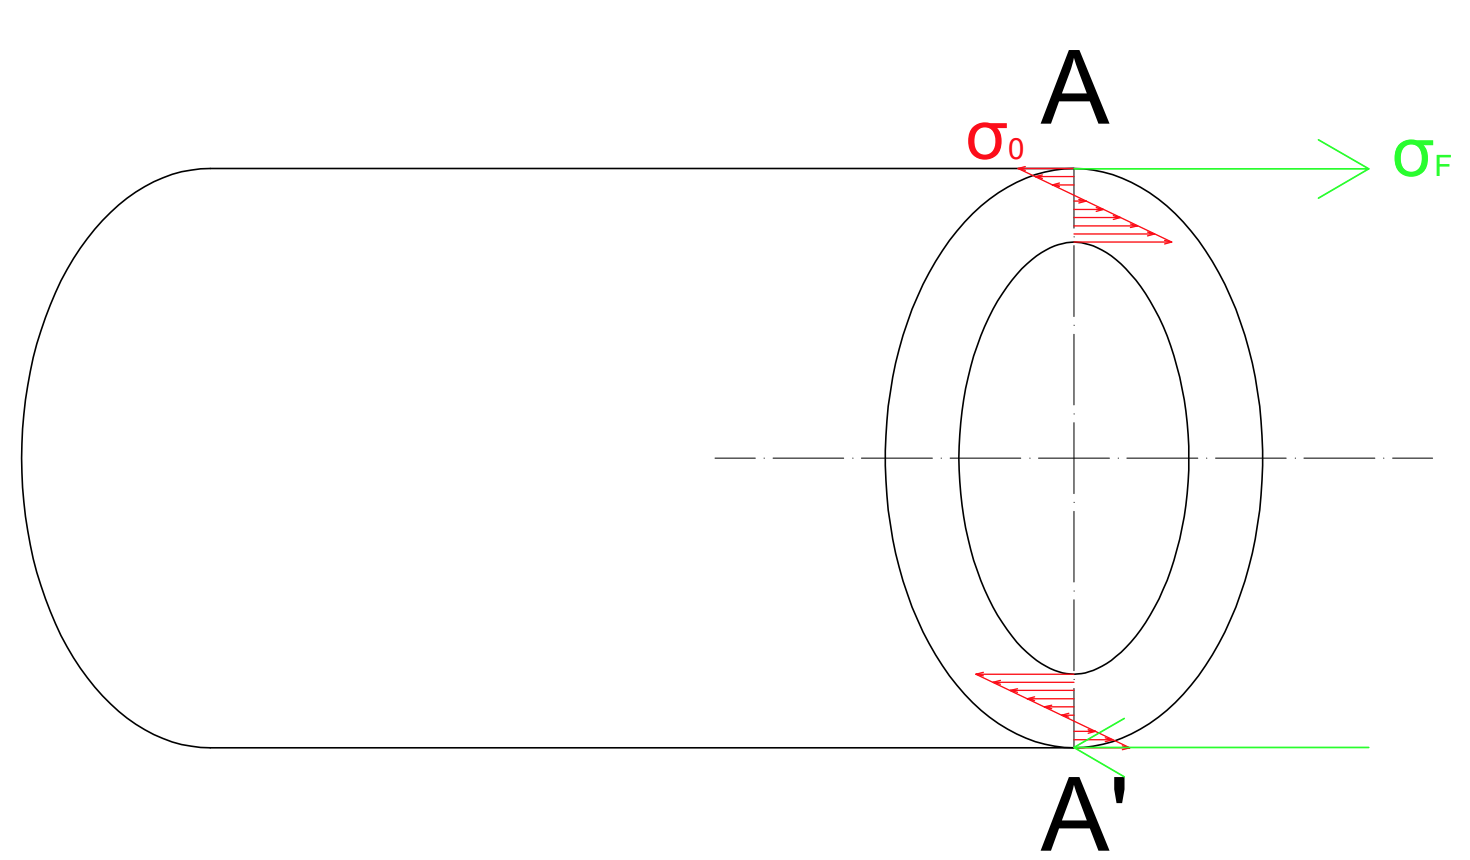
\includegraphics[scale=0.3]{Immagini/Sezione1Spinotto.png}
    \caption{Combinazione degli sforzi di flessione ed ovalizzazione}
    \label{fig:Sezione1Spinotto}
\end{figure}
\\
La sollecitazione equivalente agente in A la si calcola attraverso il criterio di Von Mises:
\begin{equation}
    \sigma_{eq_{A}}=\sqrt{\sigma_f^2+\sigma_o^2-\sigma_f\sigma_o}=138,82\ MPa.
\end{equation}
Effettuando la verifica statica si ottiene un coefficiente di sicurezza n pari a:
\begin{equation}
    n=\frac{\sigma_{amm}}{\sigma_{eq_{A}}}=4,18
\end{equation}
essendo note le caratteristiche del materiale del materiale (mat.C45 con $R_S=580\ MPa$).
\paragraph{Sezione 2}Nella seconda sezione sono presenti sollecitazioni di taglio, ovalizzazione e  flessione. Tuttavia, avendo già studiato la sezione in cui la flessione è massima, si sceglie di privilegiare il punto in cui lo stato tensionale di taglio è massimo (punto in cui la flessione è nulla).\\
Combinando i due andamenti noti delle sollecitazioni appena definite si ottiene una configurazione rappresentata in Fig.\ref{fig:Sezione2Spinotto}, dove è possibile osservare che in corrispondenza del punto B è presente lo stato di massimo sforzo.\\
\begin{figure}[h]
    \centering
    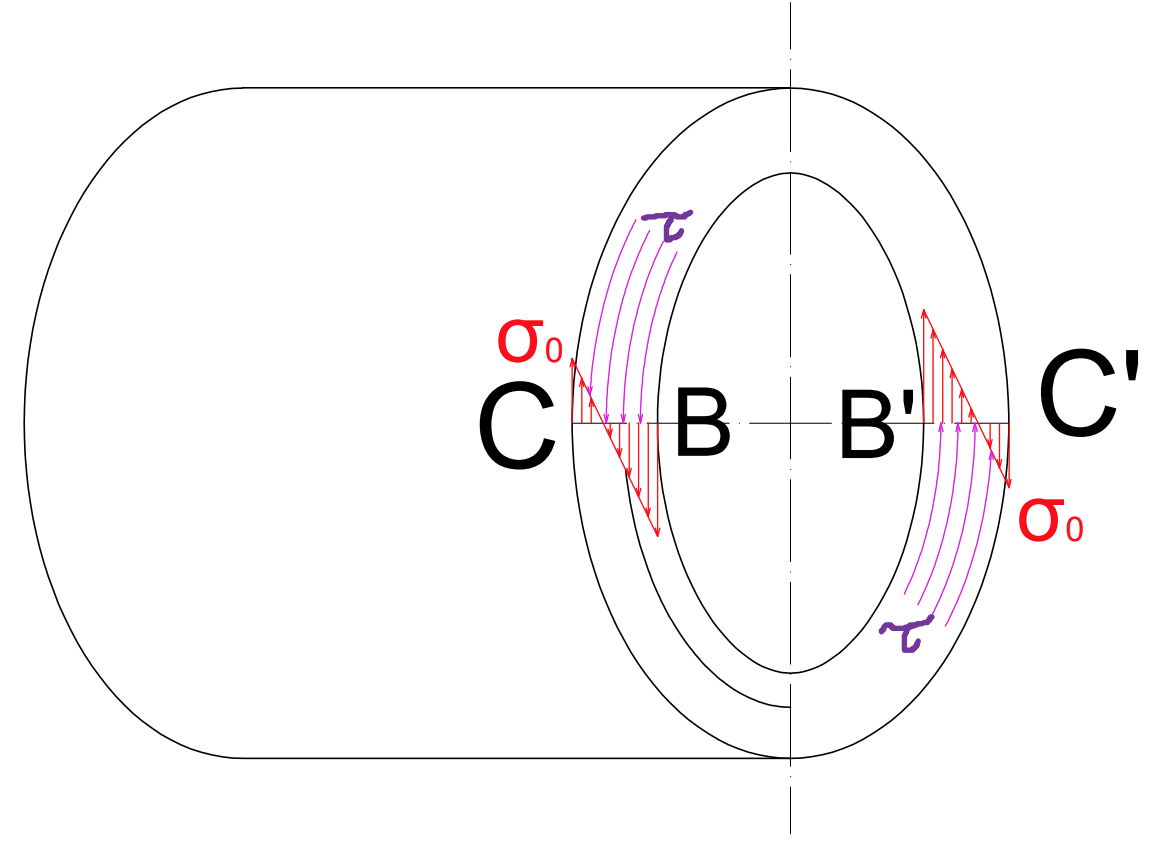
\includegraphics[scale=0.3]{Immagini/Sezione2Spinotto.png}
    \caption{Combinazione degli sforzi di taglio ed ovalizzazione}
    \label{fig:Sezione2Spinotto}
\end{figure}
\\
Osservando l'andamento della tensione di ovalizzazione e combinandolo con l'andamento costante del taglio, si deduce che il punto con maggiore criticità è quello interno, in quanto in corrispondenza di questo le sollecitazioni $\sigma_o$ e $\tau$ hanno medesimo verso.\\
La sollecitazione equivalente agente in B la si calcola attraverso il criterio di Von Mises:
\begin{equation}
    \sigma_{eq_{B}}=\sqrt{\sigma_o^2+3\tau^2}=59\ MPa.
\end{equation}
Effettuando la verifica statica si ottiene un coefficiente di sicurezza n pari a:
\begin{equation}
    n=\frac{\sigma_{amm}}{\sigma_{eq_{B}}}=9,83
\end{equation}
Il componente risulta quindi essere ampiamente verificato a livello statico. 
\subsubsection{Verifica a fatica}
Essendo la forza $F_a$ caratterizzata da un andamento variabile nel tempo, risulta necessario andare ad effettuare una verifica a fatica delle sezioni più sollecitate del componente.\\
Per i successivi calcoli si considera l'ipotesi di piccoli spostamenti per l'angolo $\beta$, trascurando la rotazione dello spinotto attorno al suo asse longitudinale.
\paragraph{Sezione 1} Si può considerare, in prima approssimazione, un ciclo di carico all'annullamento (R=0), in cui quindi si può supporre una forza minima nulla e massima pari a $F_a$. Da cui ne deriva una variabilità delle tensioni da $\sigma_{max}$ a $\sigma_{min}$ in modo sinusoidale.
\begin{itemize}
    \item $\sigma_{A,Max}=\sigma_{eq_{A}}=138,82\ MPa$
    \item $\sigma_{A,Min}\simeq0\ MPa$
    \item $\sigma_m=\sigma_a=\frac{\sigma_{A,Max}}{2}=69,41\ MPa$
\end{itemize}
\newpage
\begin{figure}[h]
    \centering
    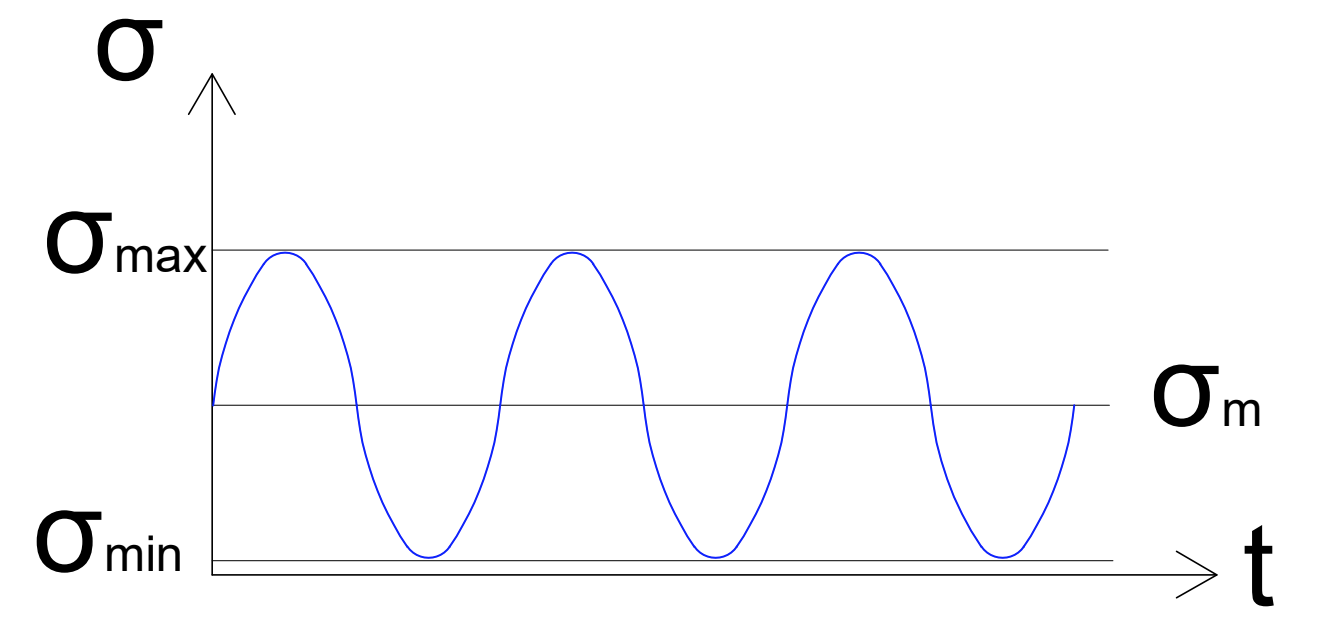
\includegraphics[scale=0.4]{Immagini/CicloFaticaSpinotto.png}
    \caption{Ciclo di carico spinotto}
    \label{fig:CicloFaticaSpinotto}
\end{figure}
È possibile ora stimare il limite di fatica con la seguente formula:
\begin{equation}
    \sigma_{w0}=0,5\cdot R_m\cdot C_{surf}\cdot C_{size}\cdot C_{load}=303,41\ MPa
\end{equation}
\begin{itemize}
    \item $C_{surf}=0,87$, da tabella in Fig.\ref{fig:CurvaCLoad} considerando rettifica 
    \item $C_{size}=1,189\cdot d^{-0,097}=0,93$
    \item $C_{load}=1$
\end{itemize}
\begin{figure}[h]
    \centering
    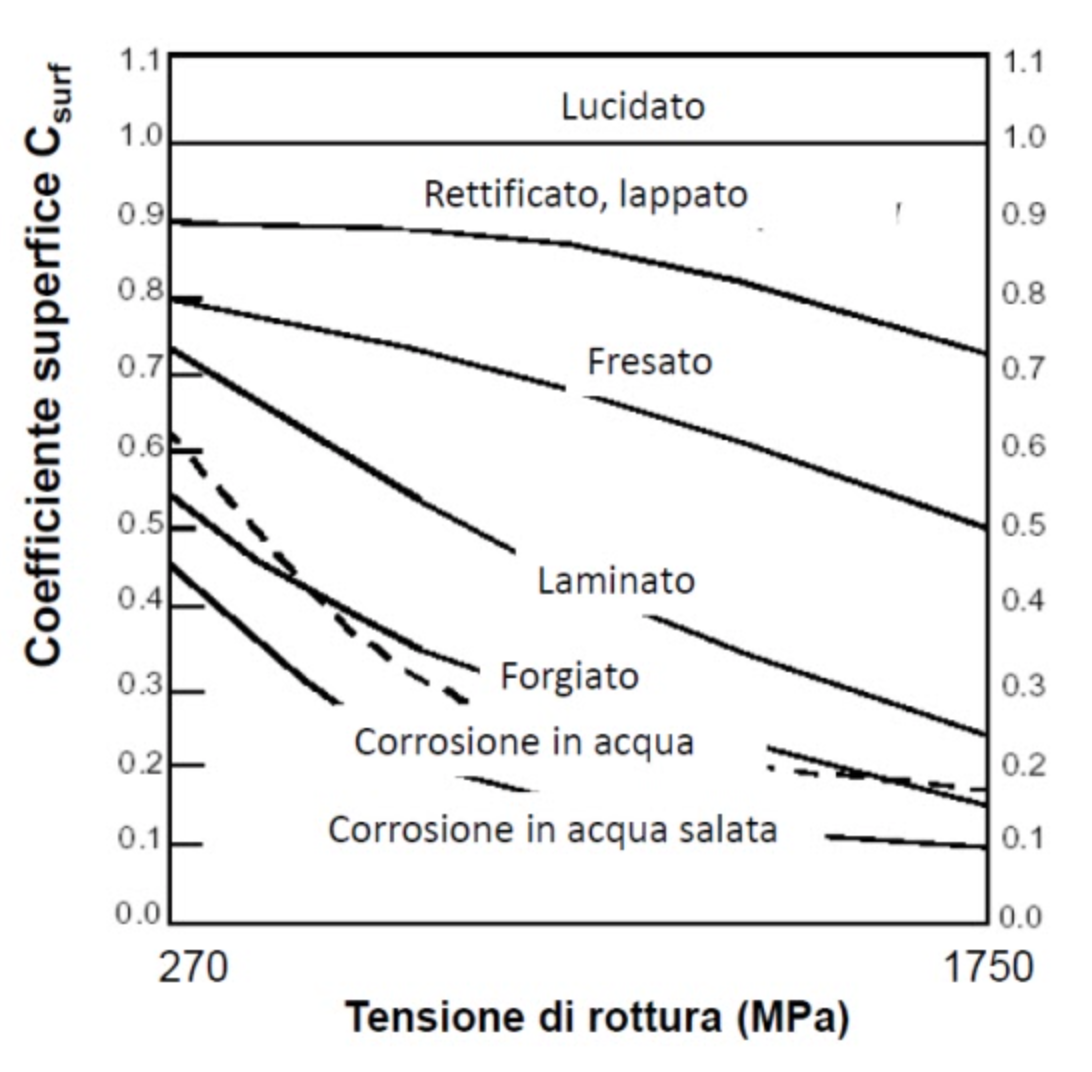
\includegraphics[scale=0.4]{Immagini/CurvaCLoad.png}
    \caption{Andamento del coefficiente $C_{surf}$}
    \label{fig:CurvaCLoad}
\end{figure}
Effettuando la verifica a fatica si ottiene un coefficiente di sicurezza n pari a:
\begin{equation}
    n=\frac{1}{\frac{\sigma_a}{\sigma_{w0}}+\frac{\sigma_m}{R_m}}=3,11
\end{equation}
\paragraph{Sezione 2}
Esattamente come per la sezione 1, si può considerare in prima approssimazione, un ciclo di carico all'annullamento (R=0), in cui quindi si può supporre una forza minima nulla e massima pari a $F_a$. Da cui ne deriva una variabilità delle tensioni da $\sigma_{max}$ a $\sigma_{min}$ in modo sinusoidale (Fig.\ref{fig:CicloFaticaSpinotto}).
\begin{itemize}
    \item $\sigma_{B,Max}=\sigma_{eq_{B}}=59\ MPa$
    \item $\sigma_{B,Min}\simeq0\ MPa$
    \item $\sigma_m=\sigma_a=\frac{\sigma_{B,Max}}{2}=29,5\ MPa$
\end{itemize}
È possibile ora stimare il limite di fatica con la seguente formula:
\begin{equation}
    \sigma_{w0}=0,5\cdot R_m\cdot C_{surf}\cdot C_{size}\cdot C_{load}=216\ MPa
\end{equation}
\begin{itemize}
    \item $C_{surf}=0,65$, da tabella in Fig.\ref{fig:CurvaCLoad} considerando trafilatura 
    \item $C_{size}=1,189\cdot d^{-0,097}=0,96$
    \item $C_{load}=1$
\end{itemize}
Effettuando la verifica a fatica si ottiene un coefficiente di sicurezza n pari a:
\begin{equation}
    n=\frac{1}{\frac{\sigma_a}{\sigma_{w0}}+\frac{\sigma_m}{R_m}}=5,6
\end{equation}
Il componente risulta quindi essere ampiamente verificato a fatica, nonostante l'approccio cautelativo adottato inizialmente.
\subsubsection{Verifica a pressioni di contatto}
In ultima analisi, si prende in considerazione l'effetto delle pressioni di contatto fra spinotto e biella.\\
Queste ultime possono essere valutate secondo la seguente formula:
\begin{equation}
    p_c=\frac{F_a}{D\cdot l_b}=6,4\ MPa\leq p_{amm}=16\ MPa
\end{equation}
dove $l_b$ corrisponde alla larghezza del piede di biella che si impegna sullo spinotto.
\begin{figure}[h]
    \centering
    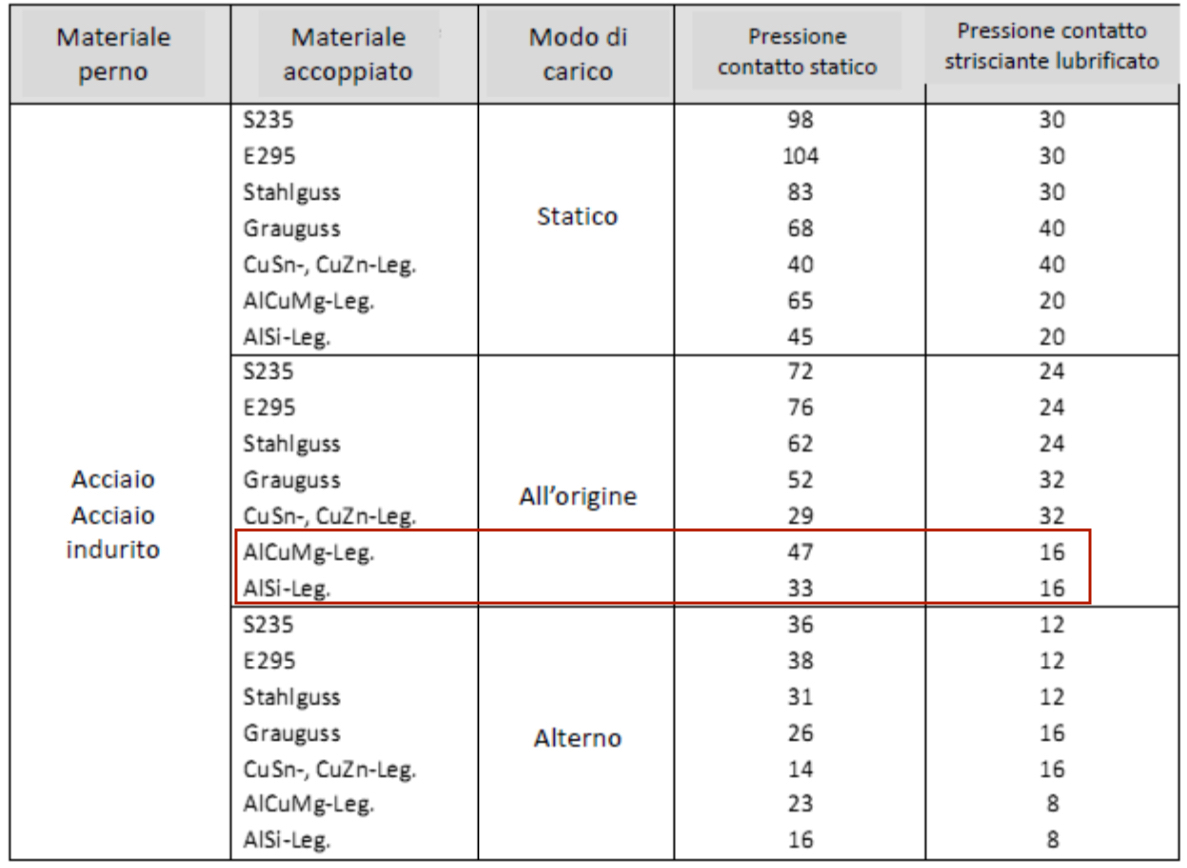
\includegraphics[scale=0.2]{Immagini/PressioniContatto.jpeg}
    \caption{Pressioni di contatto ammissibili}
    \label{fig:PressioniContatto}
\end{figure}
Il componente risulta quindi verificato alle pressioni di contatto. 
\subsection{Biella}
Si prosegue ora con l'analisi dei componenti del cinematismo focalizzando l'attenzione sulla biella. \\
Le sollecitazioni agenti sull'elemento sono molteplici:
\begin{itemize}
    \item sforzo normale
    \item impuntamento
    \item colpo di frusta
\end{itemize}
\subsubsection{Sforzo normale}
Durante il funzionamento del compressore la biella sarà soggetta ad uno sforzo normale derivante dalla pressione del fluido e dalle inerzie in gioco. L'andamento di tale sollecitazione è già stato rappresentato in Fig.\ref{fig:GraficoForzaRisultante}, dove si evince una forza massima agente sul componente assunta pari a $F_{max}=2500\ N$.\\
La sezione più sollecitata da questa sforzo sarà quella che presenta area resistente minore. La valutazione per questo parametro, unito al momento di inerzia, è stata effettuata mediante software di modellazione SOLIDWORKS. 
\begin{figure}[h]
    \centering
    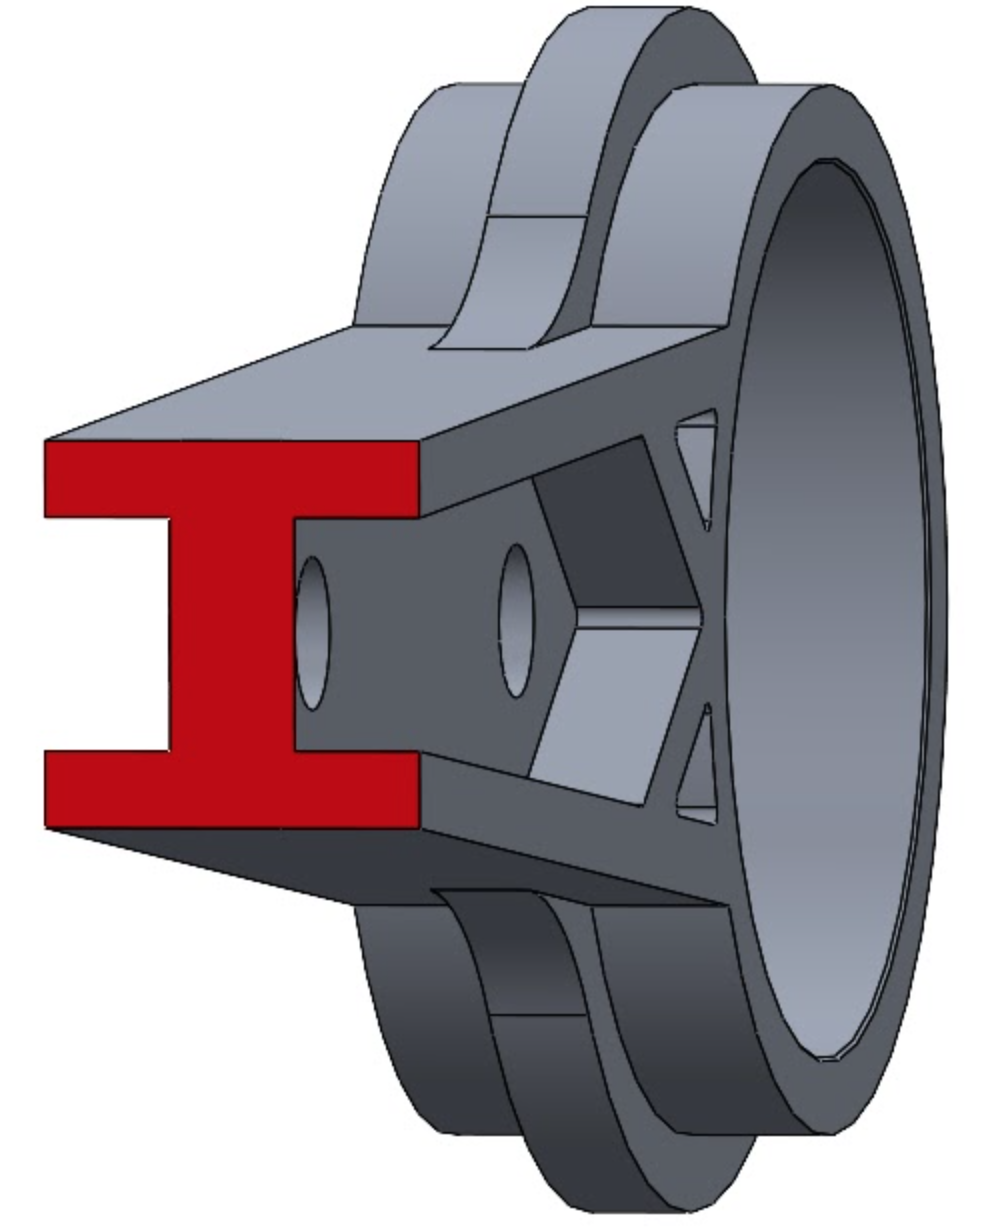
\includegraphics[scale=0.3]{Immagini/SezioneMinoreBiella1.png}
    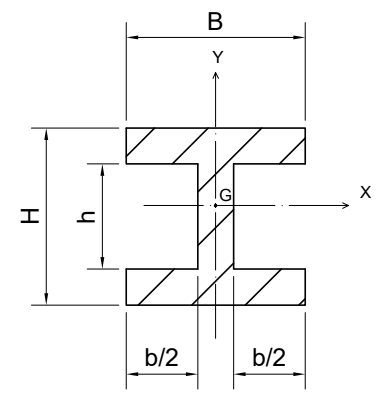
\includegraphics[scale=0.6]{Immagini/SezioneMinoreBiella2.png}
    \caption{Sezione resistente minore biella }
    \label{fig:SezioneMinoreBiella}
\end{figure}
I dati caratteristici di questa sezione sono:
\begin{itemize}
    \item Area resistente minima: $A_{min}=134,75\ mm^2$
    \item Momento di inerzia: $J_{min}=3661,9\ mm^4$
    \item Materiale: lega Al 2010-T6
    \item Carico di snervamento: $R_s=349\ MPa$
    \item Carico di rottura: $R_m=359\ MPa$
\end{itemize}
Noti questi parametri è possibile calcolare il valore del massimo stato tensionale di compressione come:
\begin{equation}
    \sigma_{max}=\left|\frac{F_{max}}{A_{min}}\right|=18,55\ MPa
\end{equation}
dalla quale si ottiene un coefficiente di sicurezza:
\begin{equation}
    n=\frac{\sigma_{amm}}{\sigma_{max}}=\frac{R_s}{\sigma_{max}}=18,81.
\end{equation}
Bisogna ricordare che tale valore deve essere sufficientemente elevato da comprendere la presenza di un foro immediatamente adiacente alla sezione considerata, che genera una riduzione dell'area resistente e una concentrazione delle tensioni. Il valore ricavato risulta quindi conforme alle considerazioni appena esposte. 
\subsubsection{Impuntamento}
Successivamente si passa ad analizzare il fenomeno di instabilità all'impuntamento. \\
Tale fenomeno si presenta nel momento in cui il carico di punta risulta maggiore del carico critico di impuntamento.
\begin{figure}[h]
    \centering
    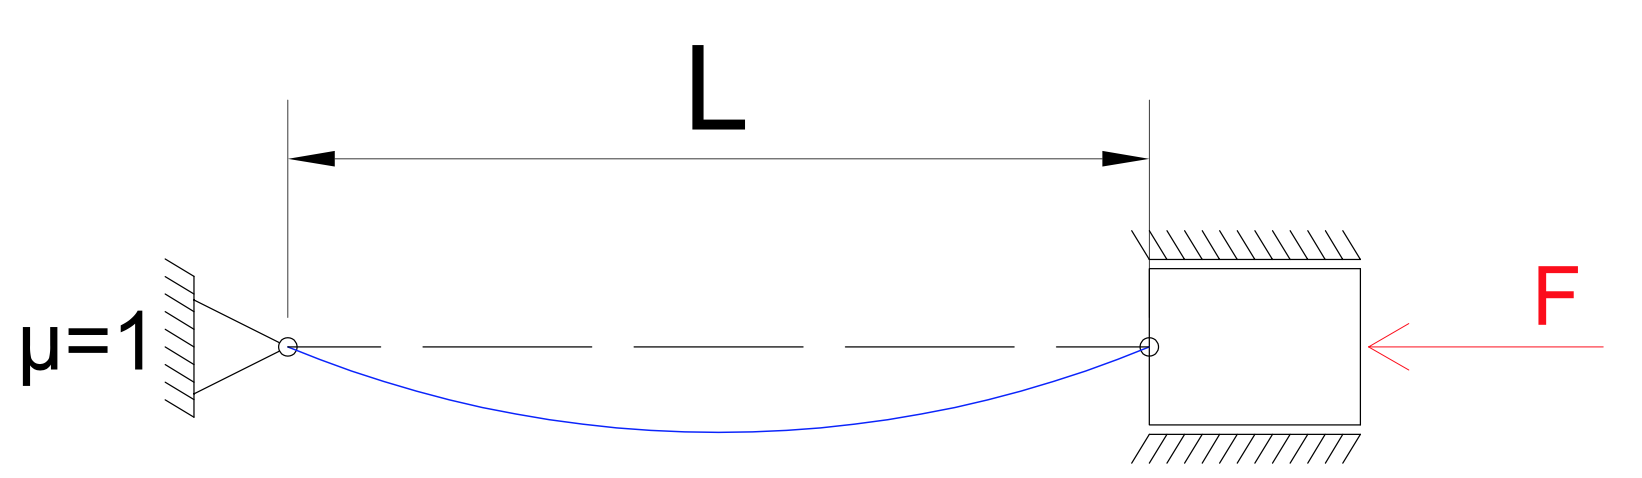
\includegraphics[scale=0.3]{Immagini/CaricoImpuntamento.png}
    \caption{Schema impuntamento della biella}
    \label{fig:CaricoImpuntamento}
\end{figure}

In primo luogo è necessario valutare la snellezza della biella identificata dal parametro:
\begin{equation}
    \lambda=5,27\cdot \frac{L}{H}=30,16
\end{equation}
dove $H=14,85\ mm$ e $L=85\ mm$.\\
\\
In generale, se $\lambda<20$ si possono trascurare fenomeni di instabilità a carico di punta e ci si può limitare a verificare la resistenza unicamente a sforzo normale.\\
\\
Nel caso in esame, essendo $20<\lambda<100$, risulta necessario effettuare una verifica all'impuntamento mediante \emph{metodo omega}.\\
\\
Tale metodo prevede il confronto di una tensione ammissibile con una tensione fittizia dipendente dal parametro $\omega$ estraibile graficamente dalla Fig \ref{fig:GraficoOmega} ($\omega=1,25$).
\newpage
\begin{figure}[h]
    \centering
    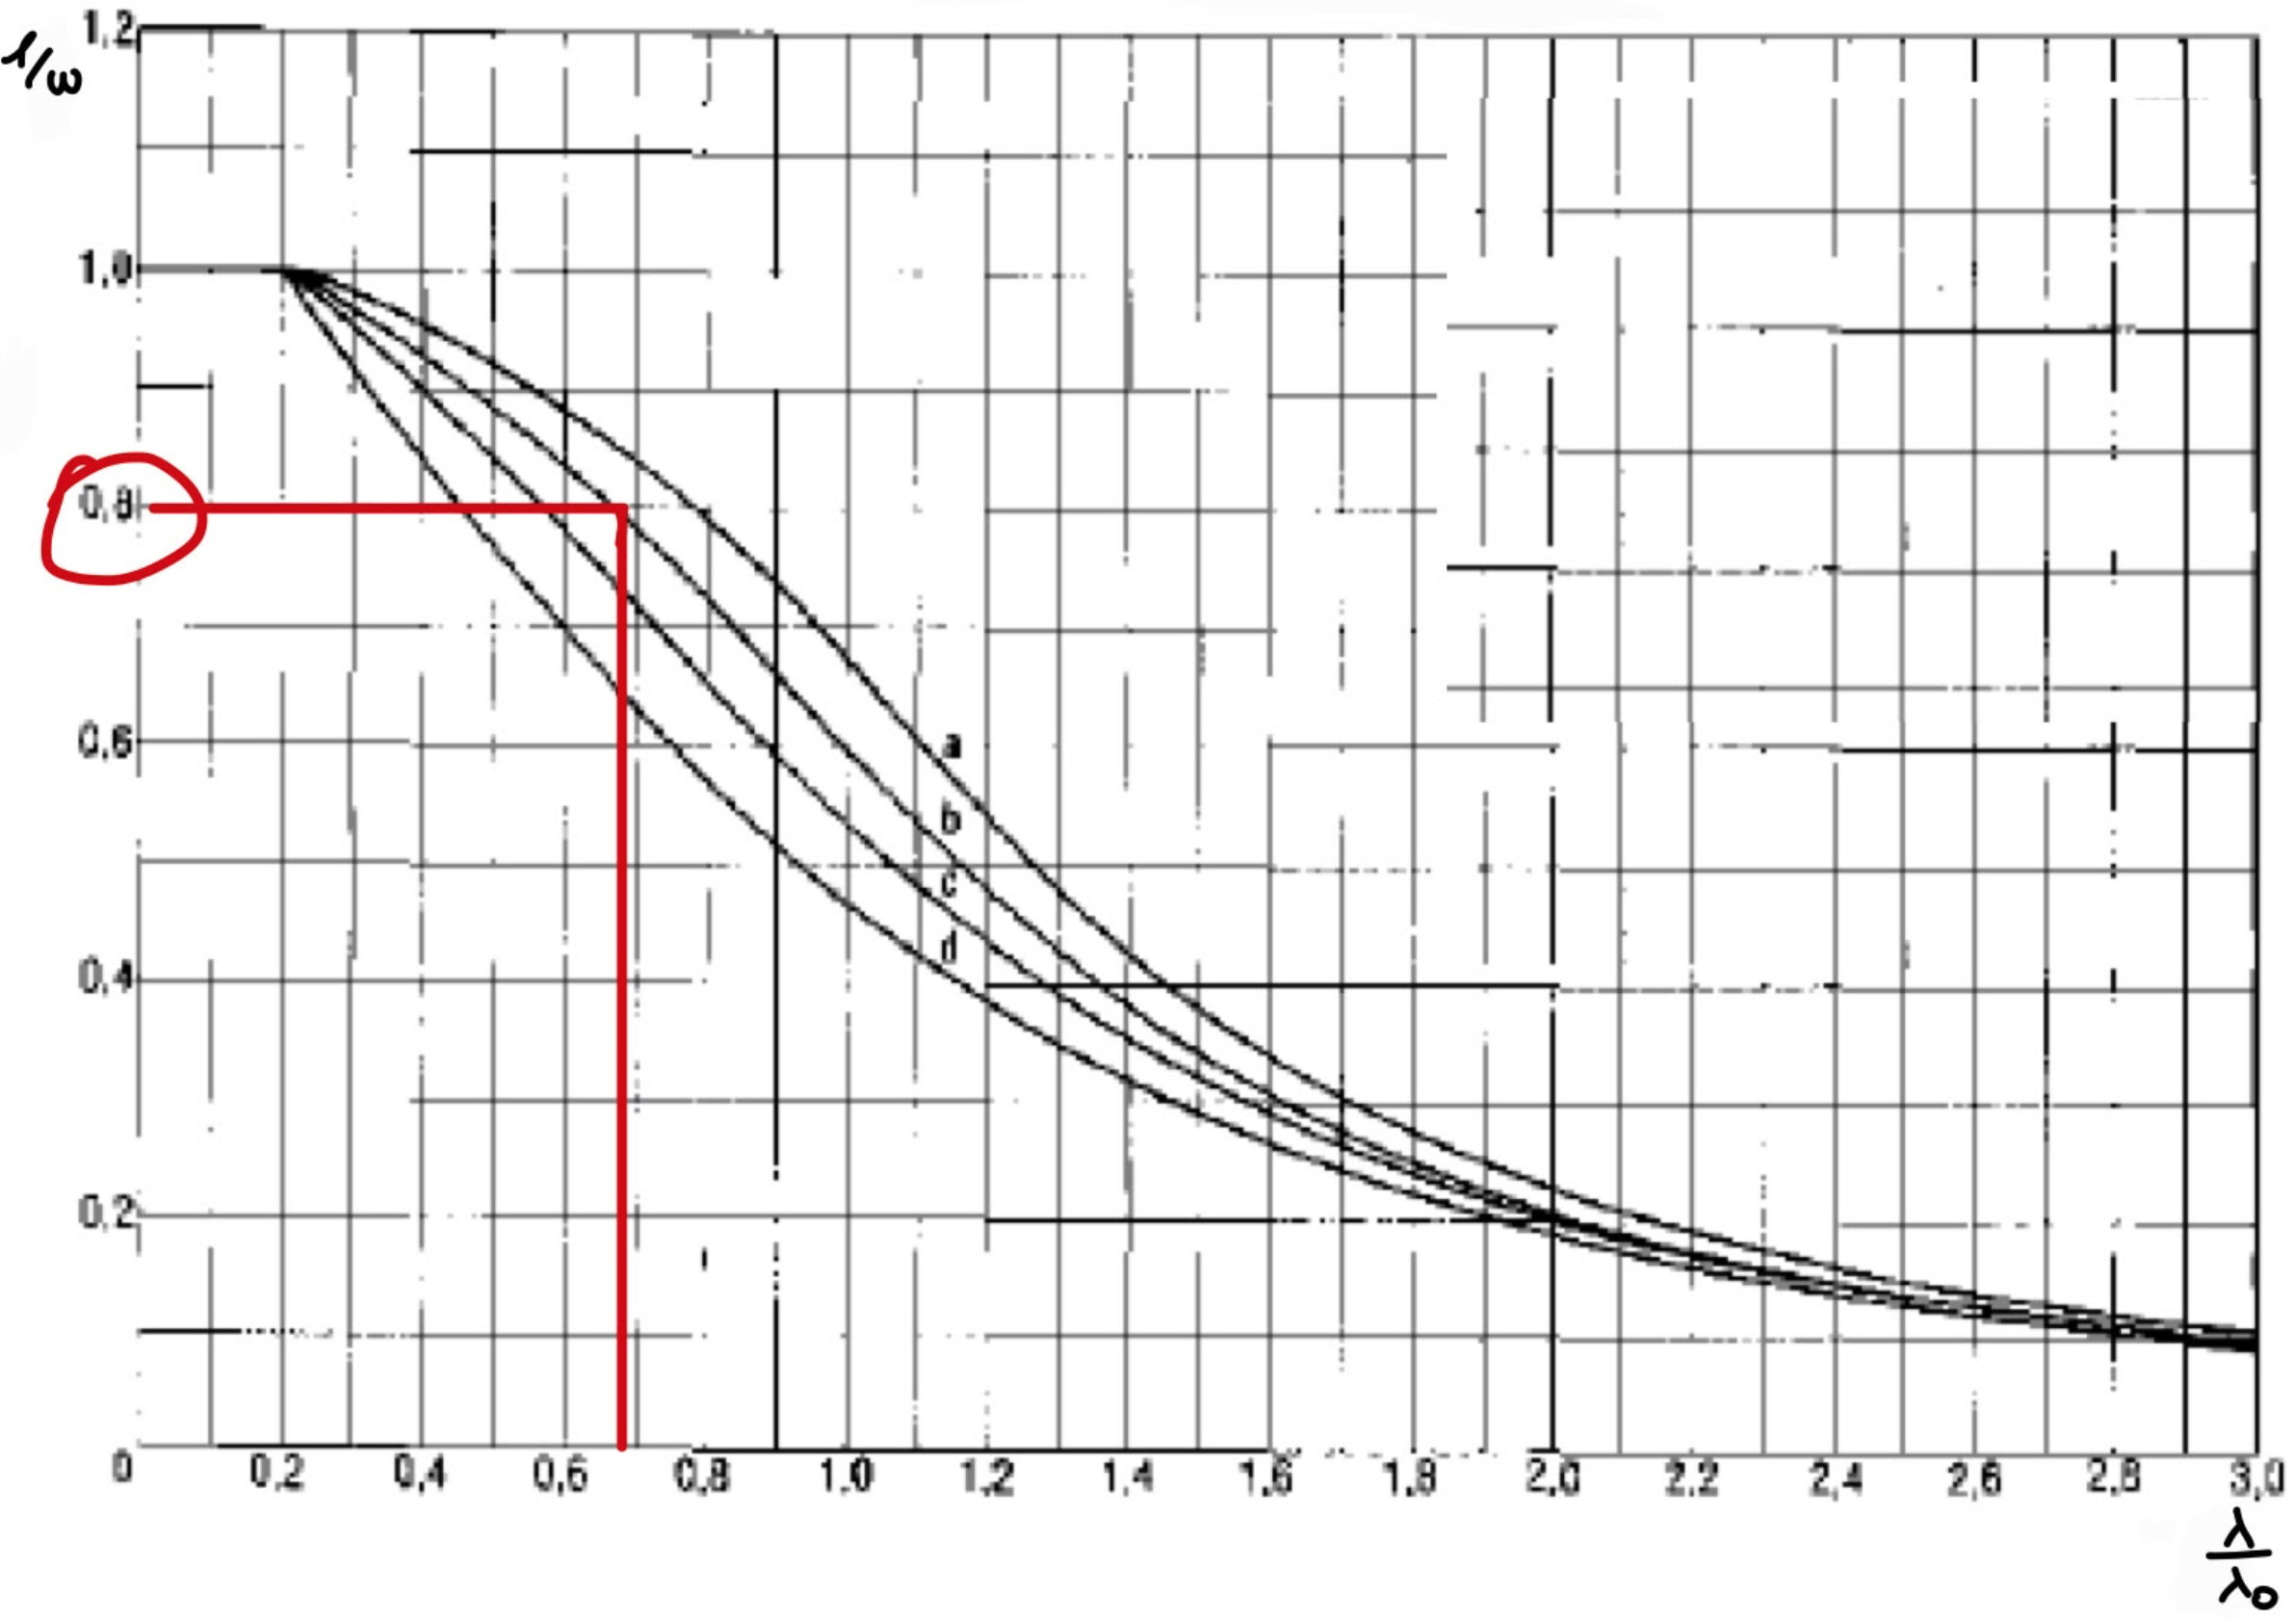
\includegraphics[scale=0.2]{Immagini/GraficoOmega.png}
    \caption{Grafico di $omega$ in funzione della snellezza}
    \label{fig:GraficoOmega}
\end{figure}

La tensione fittizzia risulta essere pari a:
\begin{equation}
    \sigma_f=\omega\cdot \frac{F_{max}}{A_{min}}=23,19\ MPa
\end{equation}
dalla quale si ottiene un coefficiente di sicurezza:
\begin{equation}
    n=\frac{\sigma_{amm}}{\sigma_{f}}=\frac{R_s}{\sigma_{f}}=15
\end{equation}
Il componente risulta quindi verificato all'impuntamento.
\subsubsection{Colpo di frusta}
Ulteriormente occorre verificare la biella a flesso-compressione nella posizione di quadratura (quando forma un angolo di 90° con la manovella).
\begin{figure}[h]
    \centering
    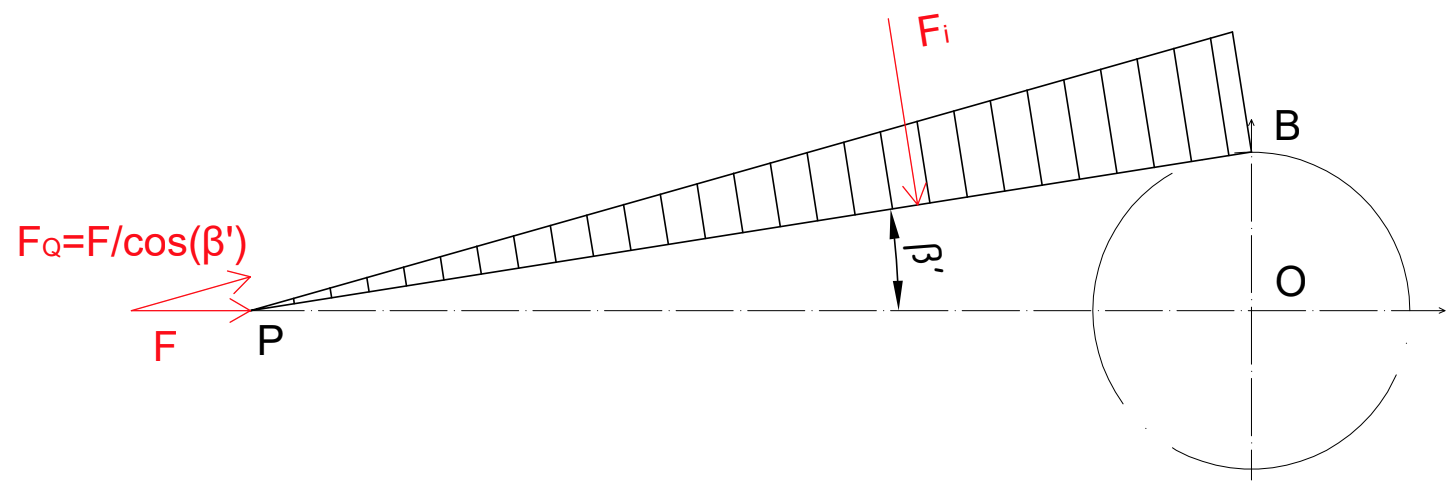
\includegraphics[scale=0.35]{Immagini/QuadraturaBiella1.png}
    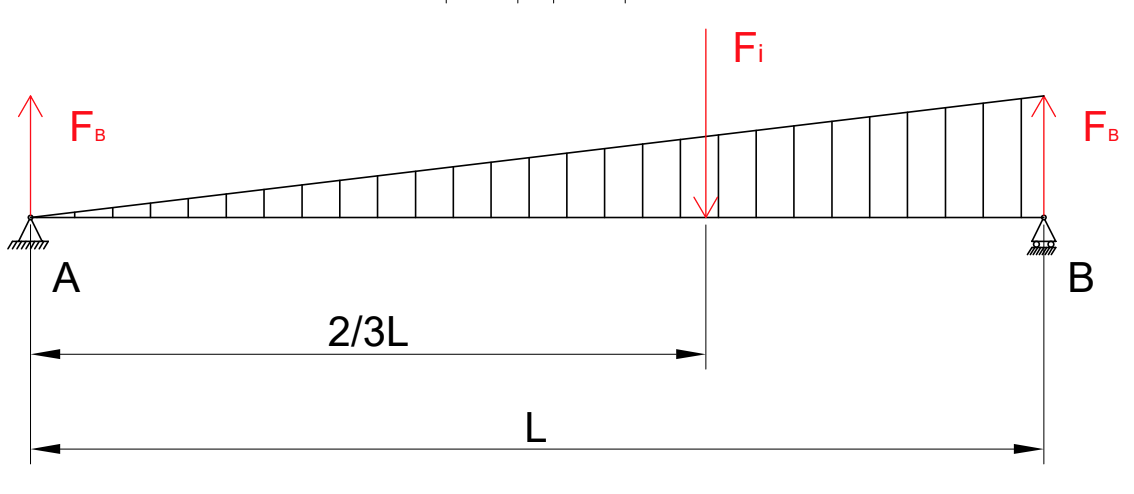
\includegraphics[scale=0.35]{Immagini/QuadraturaBiella2.png}
    \caption{Schema di biella nella posizione di quadratura}
    \label{fig:QuadraturaBiella}
\end{figure}

Osservando la Fig.\ref{fig:QuadraturaBiella} si nota che la biella è soggetta ad un moto composto da una traslazione ed una rotazione e i suoi punti sono sottoposti ad accelerazione con una componente diretta normalmente alla biella, che è massima nella posizione di quadratura. La componente trasversale dell'accelerazione è massima nel punto B ($a_B=\omega^2\cdot r$) e nulla nel punto P; un punto X distante x da quest'ultimo ha accelerazione $a_X=\omega^2\cdot r\left(x/L\right)$.\\
Ne consegue che la biella risulta essere sottoposta ad un carico distribuito triangolare, il cui momento flettente massimo si ha in una sezione distante $\frac{1}{\sqrt{3L}}$ dal punto P, e vale:
\begin{equation}
    M_{f,max}=0,064\cdot m_b\cdot \omega^2\cdot r\cdot L=156351\ N\cdot mm
\end{equation}
dove $m_b=51,61\ g$, $\omega=161,27\ rad/s$, $r=21\ mm$ e $L=85\ mm$.
La verifica si effettua con la seguente relazione:
\begin{equation}
    \sigma_{max}=\frac{F_{max}}{A_{\frac{3}{5}}\cos \beta'}+\frac{M_{f,max}}{W_{\frac{3}{5}}}\le \sigma_{amm}
    \label{colpodifrusta}
\end{equation}
in cui:
\begin{itemize}
    \item $A_{\frac{3}{5}}=160\ mm^2$ è l'area della sezione della biella a 3/5 della sua lunghezza, ottenuta mediante SOLIDWORKS
    \item $W_{\frac{3}{5}}=\frac{J}{B/2}=1027,83\ mm^3$ è il modulo di resistenza a flessione , $J=7708,75\ mm^4$  corrisponde al momento di inerzia e $B=15\ mm$ della sezione valutata mediante SOLIDWORKS
    \item $\beta'$ l'angolo per cui si verifica la quadratura che si calcola come $\beta'=\arctan(r/L)=13,88^\circ$
\end{itemize}
\begin{figure}[h]
    \centering
    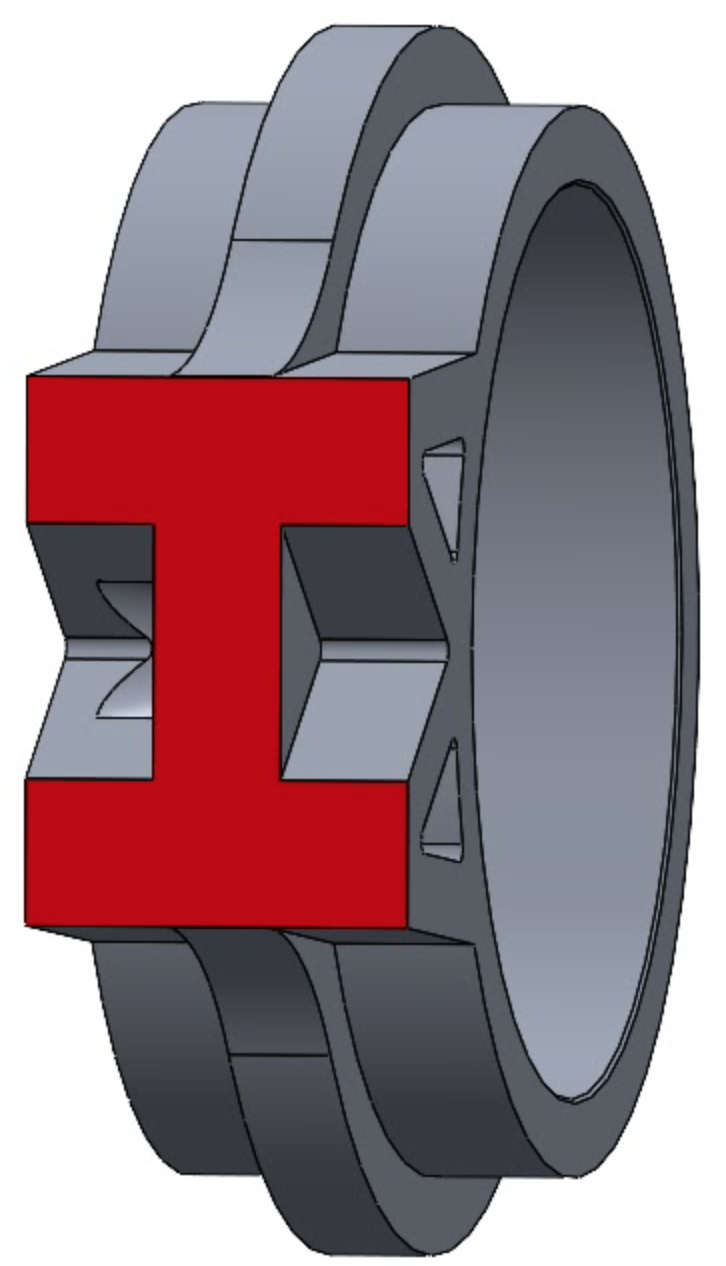
\includegraphics[scale=0.3]{Immagini/SezioneColpoFrustaBiella.png}
    \caption{Sezione della biella maggiormente sottoposta a colpo di frusta}
    \label{fig:SezioneColpoFrustaBiella}
\end{figure}
Sostituendo questi parametri all'interno dell'eq.(\ref{colpodifrusta}) si ottiene:
\begin{equation}
    \sigma_{max}=168\ MPa
\end{equation}
per cui si ottiene un fattore di sicurezza:
\begin{equation}
    n=\frac{\sigma_{amm}}{\sigma_{max}}=\frac{R_s}{\sigma_{max}}=2,1. 
\end{equation}
Il componente risulta quindi verificato al colpo di frusta.
\subsubsection{Verifica a fatica}
Essendo la forza $F_{max}$ caratterizzata da un andamento variabile nel tempo, risulta necessario andare ad effettuare una verifica a fatica della sezione più sollecitata del componente, ovvero quella in corrispondenza del foro in prossimità del piede di biella ($A_{foro}$).
\begin{figure}[h]
    \centering
    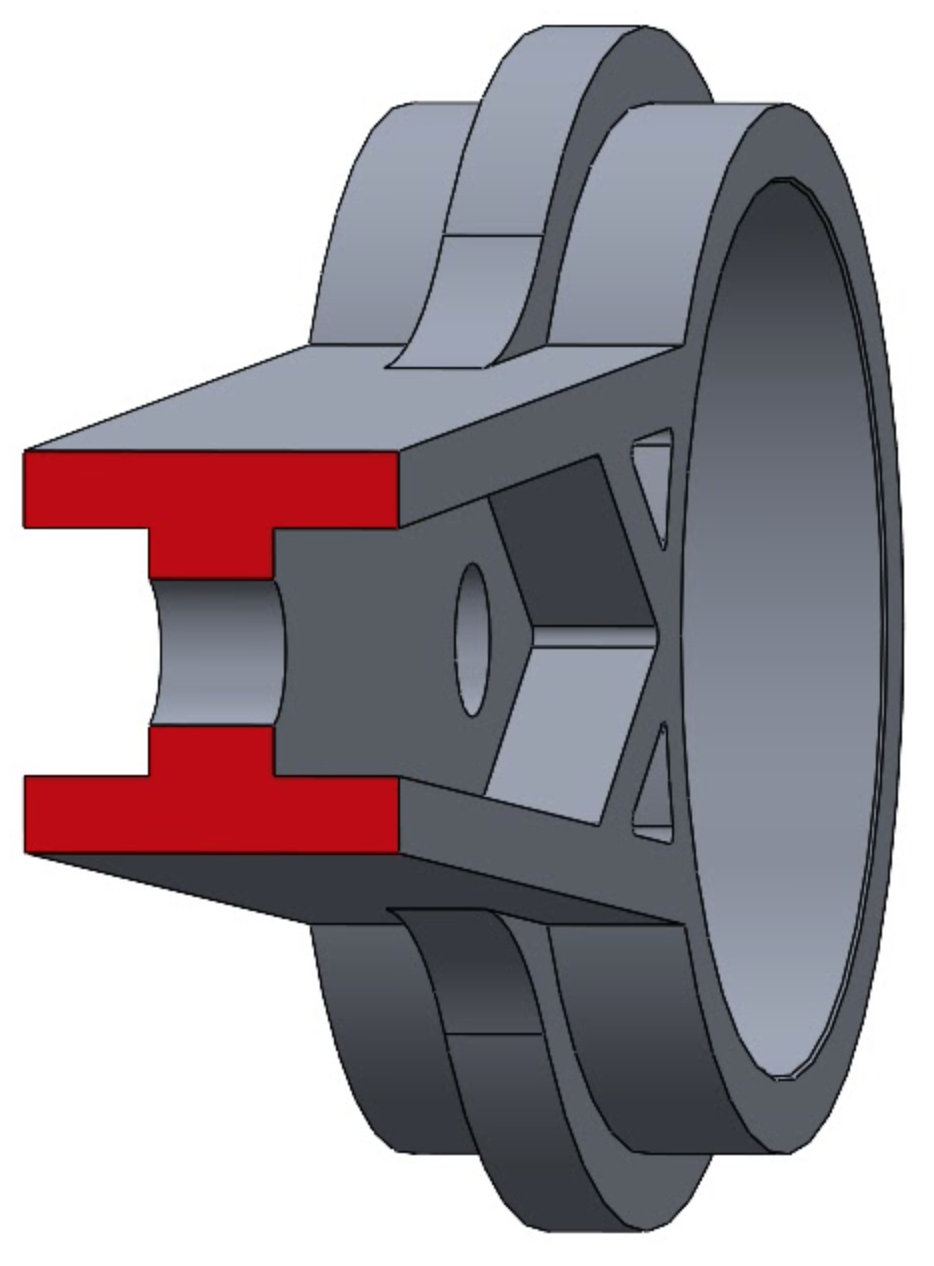
\includegraphics[scale=0.3]{Immagini/SezioneForoBiella.png}
    \caption{Sezione in corrispondenza del foro, vicina al piede di biella}
    \label{fig:SezioneForoBiella}
\end{figure}

I dati caratteristici di questa sezione sono:
\begin{itemize}
    \item Area resistente minima: $A_{foro}=104,75\ mm^2$
    \item Materiale: lega Al 2010-T6
    \item Carico di snervamento: $R_s=349\ MPa$
    \item Carico di rottura: $R_m=359\ MPa$
\end{itemize}
Si può considerare, in prima approssimazione, l'ininfluenza della sollecitazione flessionale dovuta al colpo di frusta, considerando quindi la biella unicamente soggetta a forze normali. \\
La forza massima sarà dovuta alla risultante agente di massima compressione, la forza minima sarà una forza di trazione dovuta all'inerzia in prossimità del termine della fase di discesa. 
Da cui ne deriva una variabilità delle tensioni da $\sigma_{max}$ a $\sigma_{min}$ in modo pressoché sinusoidale,
ne risulta il seguente andamento del ciclo di carico:
\begin{figure}[h]
    \centering
    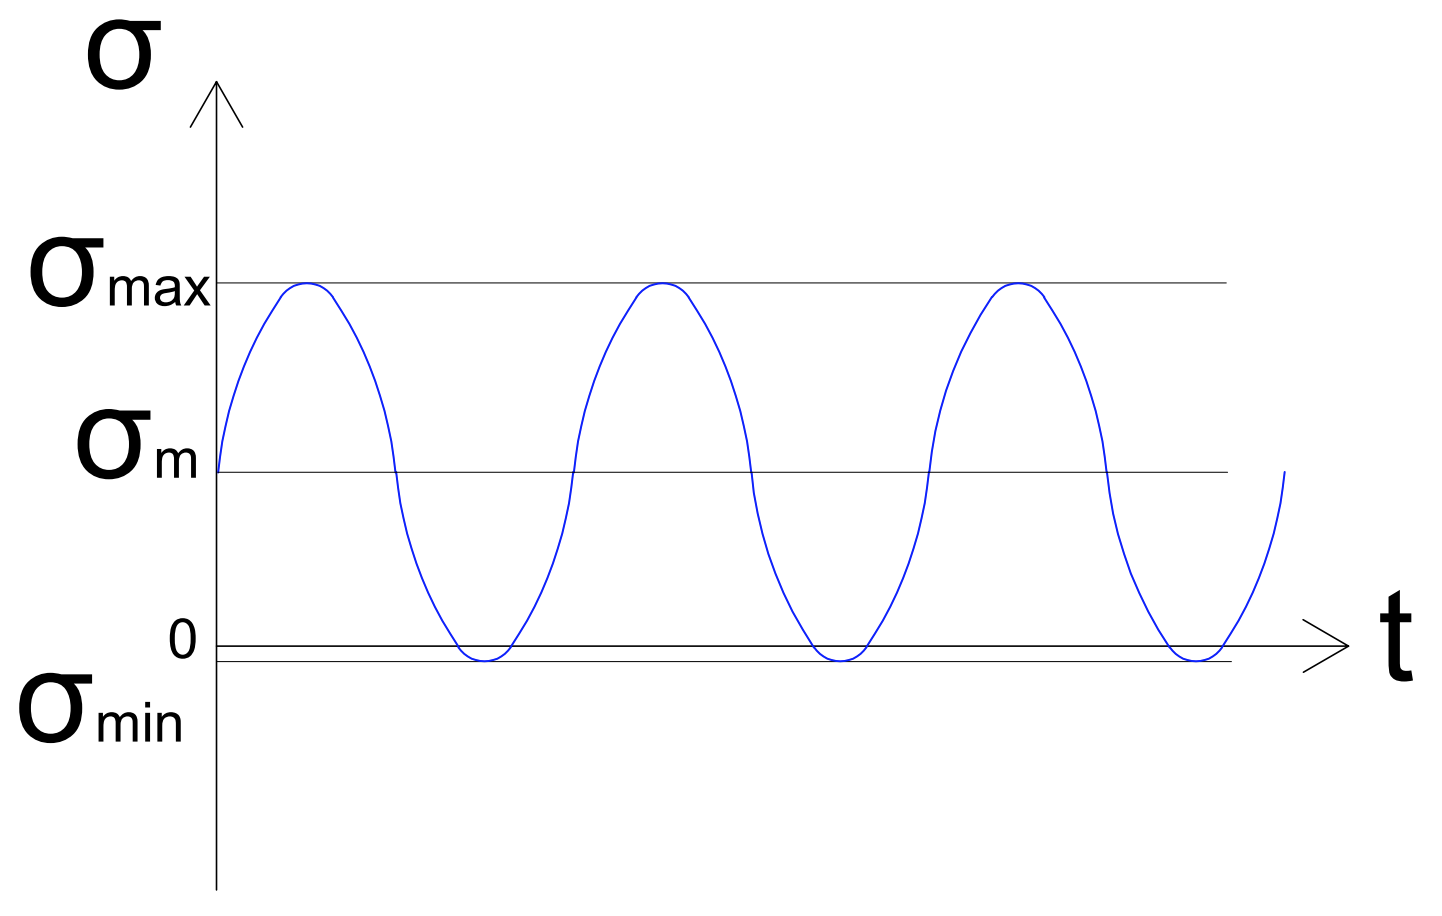
\includegraphics[scale=0.27]{Immagini/CicloFaticaBiella.png}
    \caption{Ciclo di carico biella}
    \label{fig:CicloFaticaBiella}
\end{figure}
\begin{itemize}
    \item $\sigma_{max}=\frac{F_{max}}{A_{foro}}=23,86\ MPa$
    \item $\sigma_{min}=\frac{F_{min}}{A_{foro}}=-0,66\ MPa$
    \item $\sigma_m=\frac{\sigma_{max}+\sigma_{min}}{2}=11,6\ MPa$
    \item $\sigma_a=\sigma_{max}-\sigma_m=12,26\ MPa$
\end{itemize}

È possibile ora stimare il limite di fatica con la seguente formula:
\begin{equation}
    \sigma_{w0}=0,5\cdot R_m\cdot C_{surf}\cdot C_{size}\cdot C_{load}=88,9\ MPa
\end{equation}
dove:
\begin{itemize}
    \item $C_{surf}=0,5$, da tabella in Fig.\ref{fig:CurvaCLoad} considerando forgiatura/pressofusione 
    \item $C_{size}=1,189\cdot d_{eq}^{-0,097}=0,99$ dove $d_{eq}=\frac{4A_{foro}}{2p}=6,19\ mm$ 
    \item $C_{load}=1$
\end{itemize}
Si considera un fattore di intaglio statico dovuto alla presenza del foro pari a $K_t=2,2$ ricavato tramite Fig.\ref{fig:KtBiella}.
\begin{figure}[h]
    \centering
    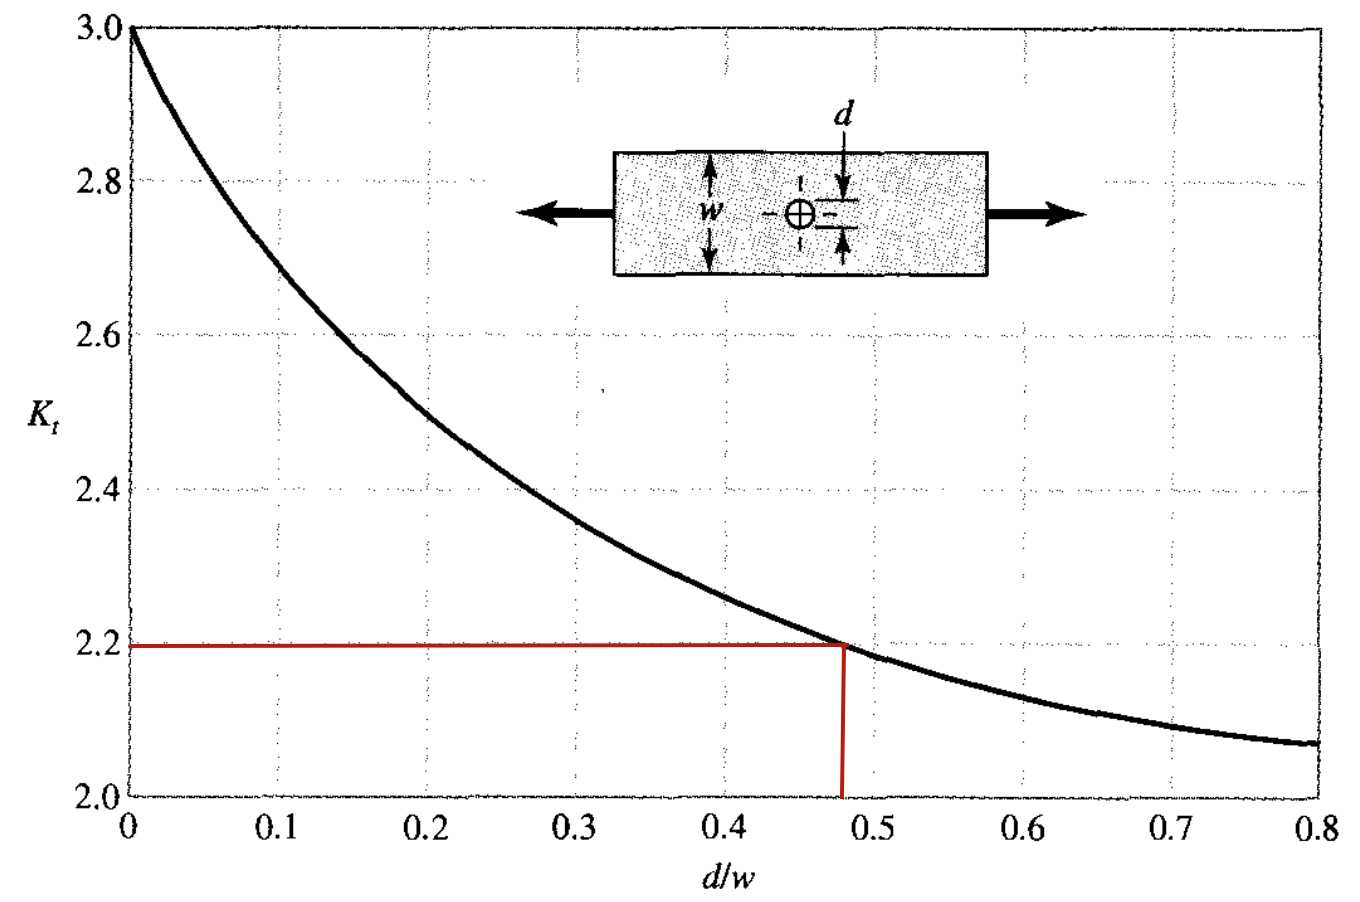
\includegraphics[scale=0.25]{Immagini/KtBiella.png}
    \caption{Grafico Kt considerato per la biella}
    \label{fig:KtBiella}
\end{figure}

Con tale fattore è possibile calcolare il fattore di intaglio a fatica:
\begin{equation}
    K_f=q\left(K_t-1\right)+1=1,95
\end{equation}
dove $q=0,79$ ricavato mediante Fig.\ref{fig:KfBiella}
\begin{figure}[h]
    \centering
    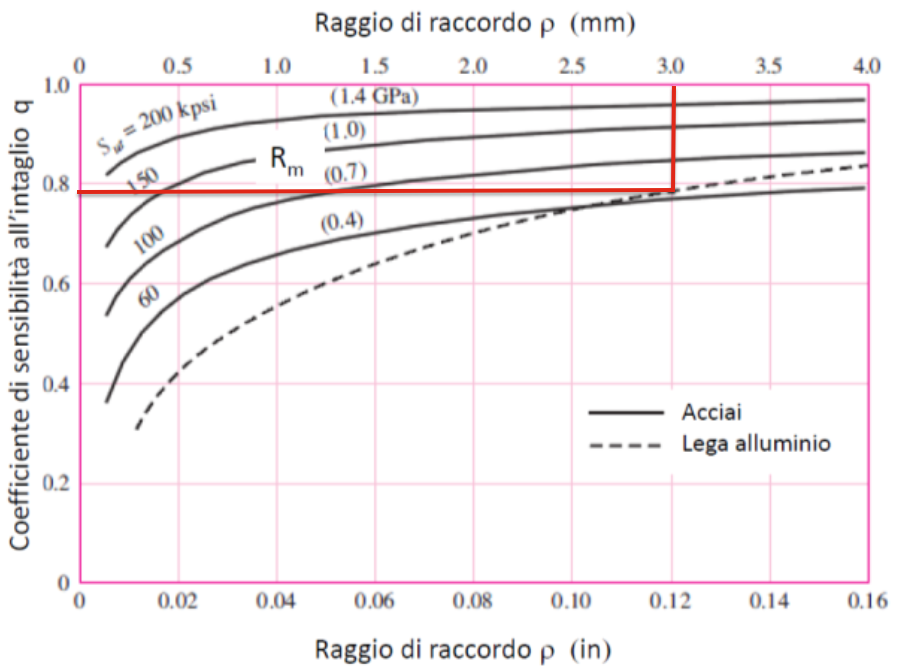
\includegraphics[scale=0.4]{Immagini/KfBiella.png}
    \caption{Grafico q in funzione del raggio }
    \label{fig:KfBiella}
\end{figure}

In conclusione, si ottiene un coefficiente di sicurezza a fatica calcolato mediante:
\begin{equation}
    n=\frac{1}{\frac{K_f\sigma_a}{\sigma_{w0}}+\frac{\sigma_m}{R_m}}=3,3.
\end{equation}
Il componente risulta quindi verificato a fatica. 
\subsection{Albero a gomiti}
In conclusione si procede con la verifica dell'albero a gomiti. Per studiare tale componente è necessario considerare l'andamento delle forze scaricate sullo stesso in funzione dell'angolo di manovella, rappresentate in Fig.\ref{fig:GraficoReazioniScaricateAlbero}.\\
Poiché le manovelle sono sfasate di 180°, nell'istante in cui la forza agente su una manovella raggiunge il suo valore massimo pari a $F_{max}=2500\ N$, si ha un valore di forza minimo agente sull'altra pari a $F_{min}=70\ N$.\\
Si possono quindi individuare due configurazioni tali per cui la forza agente è massima:
\begin{itemize}
    \item configurazione A ($\alpha\simeq 2,45\ rad$), la forza massima è scaricata in corrispondenza della manovella 2, cioè più vicina alla sede della linguetta.
    \item configurazione B ($\alpha\simeq 2,45+\pi\ rad$), la forza massima è scaricata in corrispondenza della manovella 1, cioè la più lontana dalla sede della linguetta.
\end{itemize}
\begin{figure}[h]
    \centering
    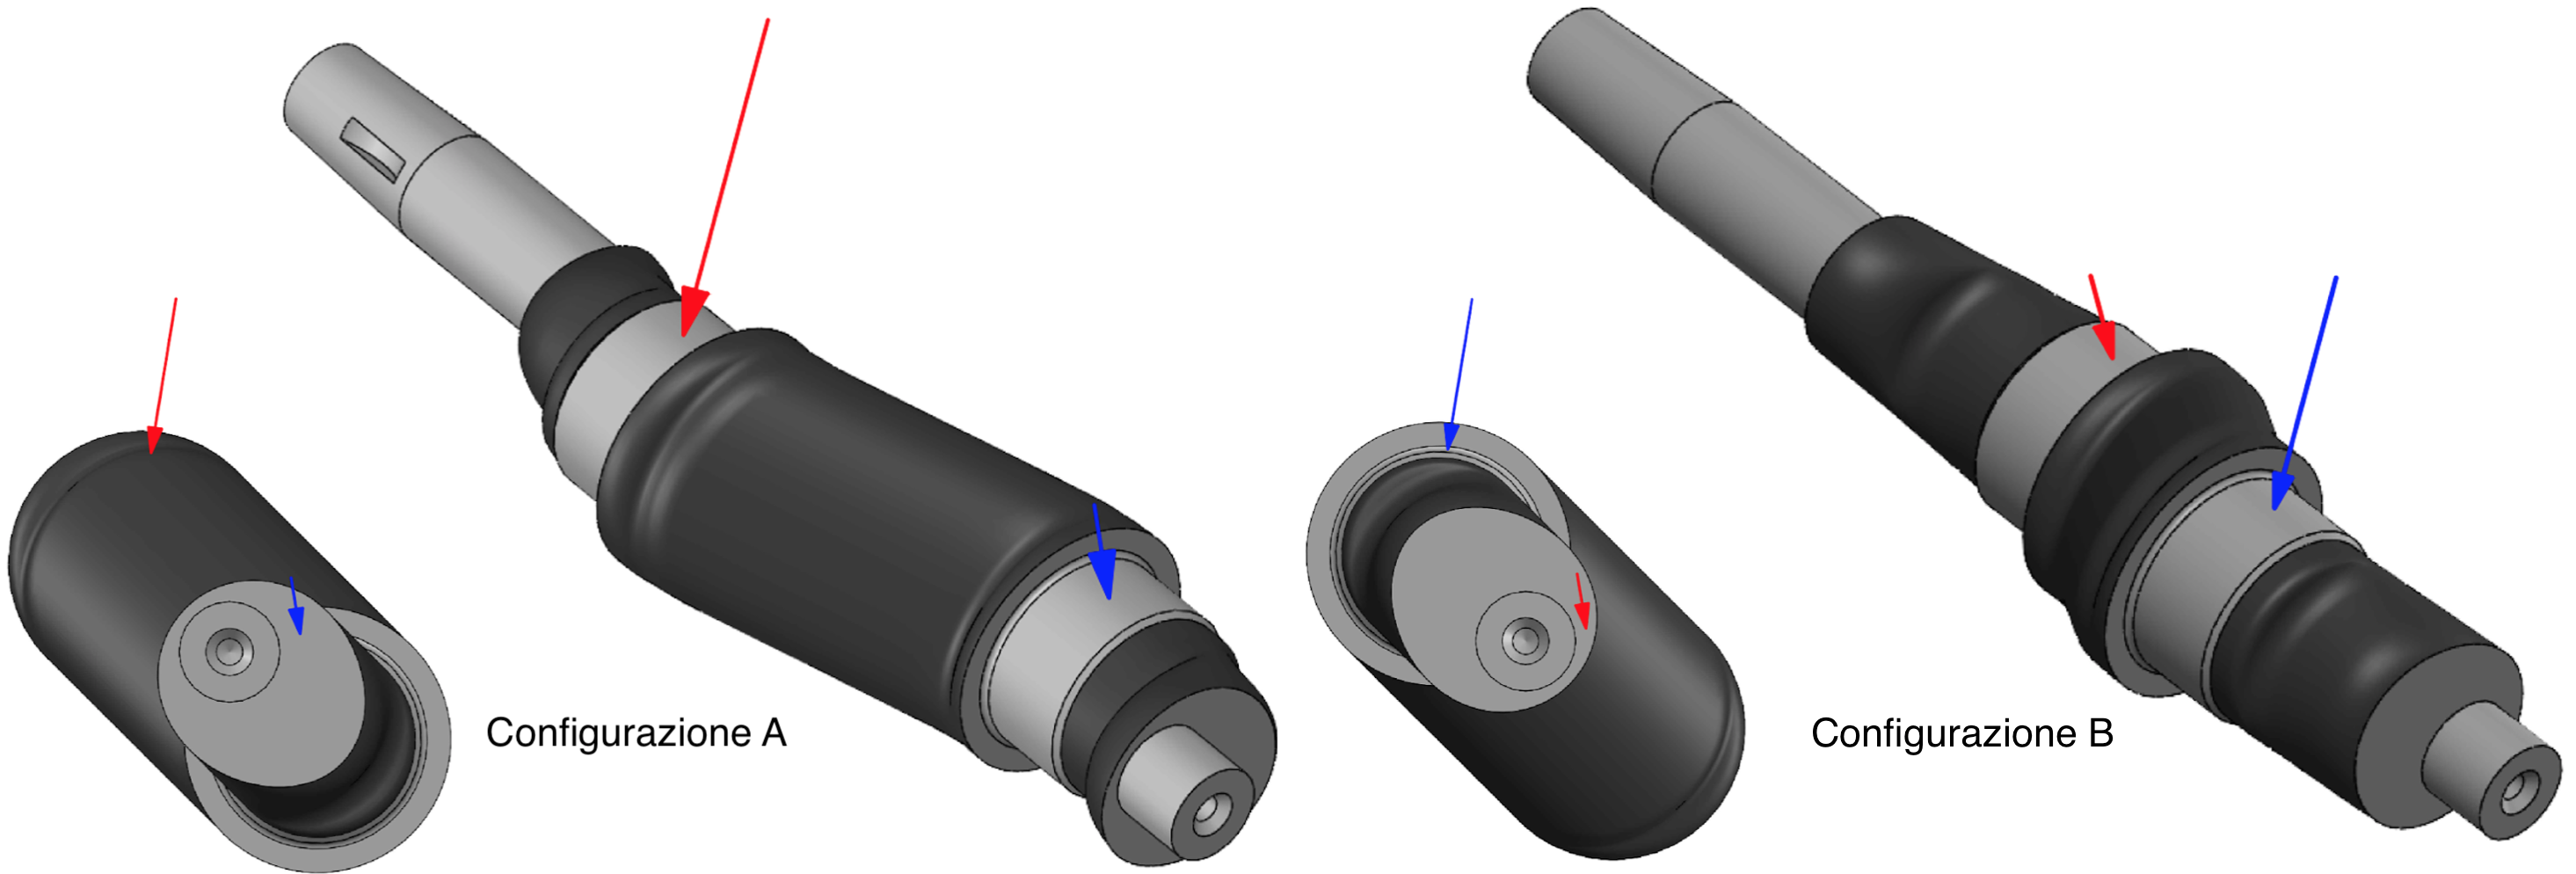
\includegraphics[scale=0.3]{Immagini/ConfigurazioneAlberoAB.png}
    \caption{Configurazione A e B dell'albero a gomiti}
    \label{fig:ConfigurazioneAlberoAB}
\end{figure}
La forza massima considerata ha sempre direzione parallela all'asse della biella, e dovrà quindi essere scomposta in due componenti come in Fig.\ref{fig:ScomposizioneForzeAlbero}.
\begin{figure}[h]
    \centering
    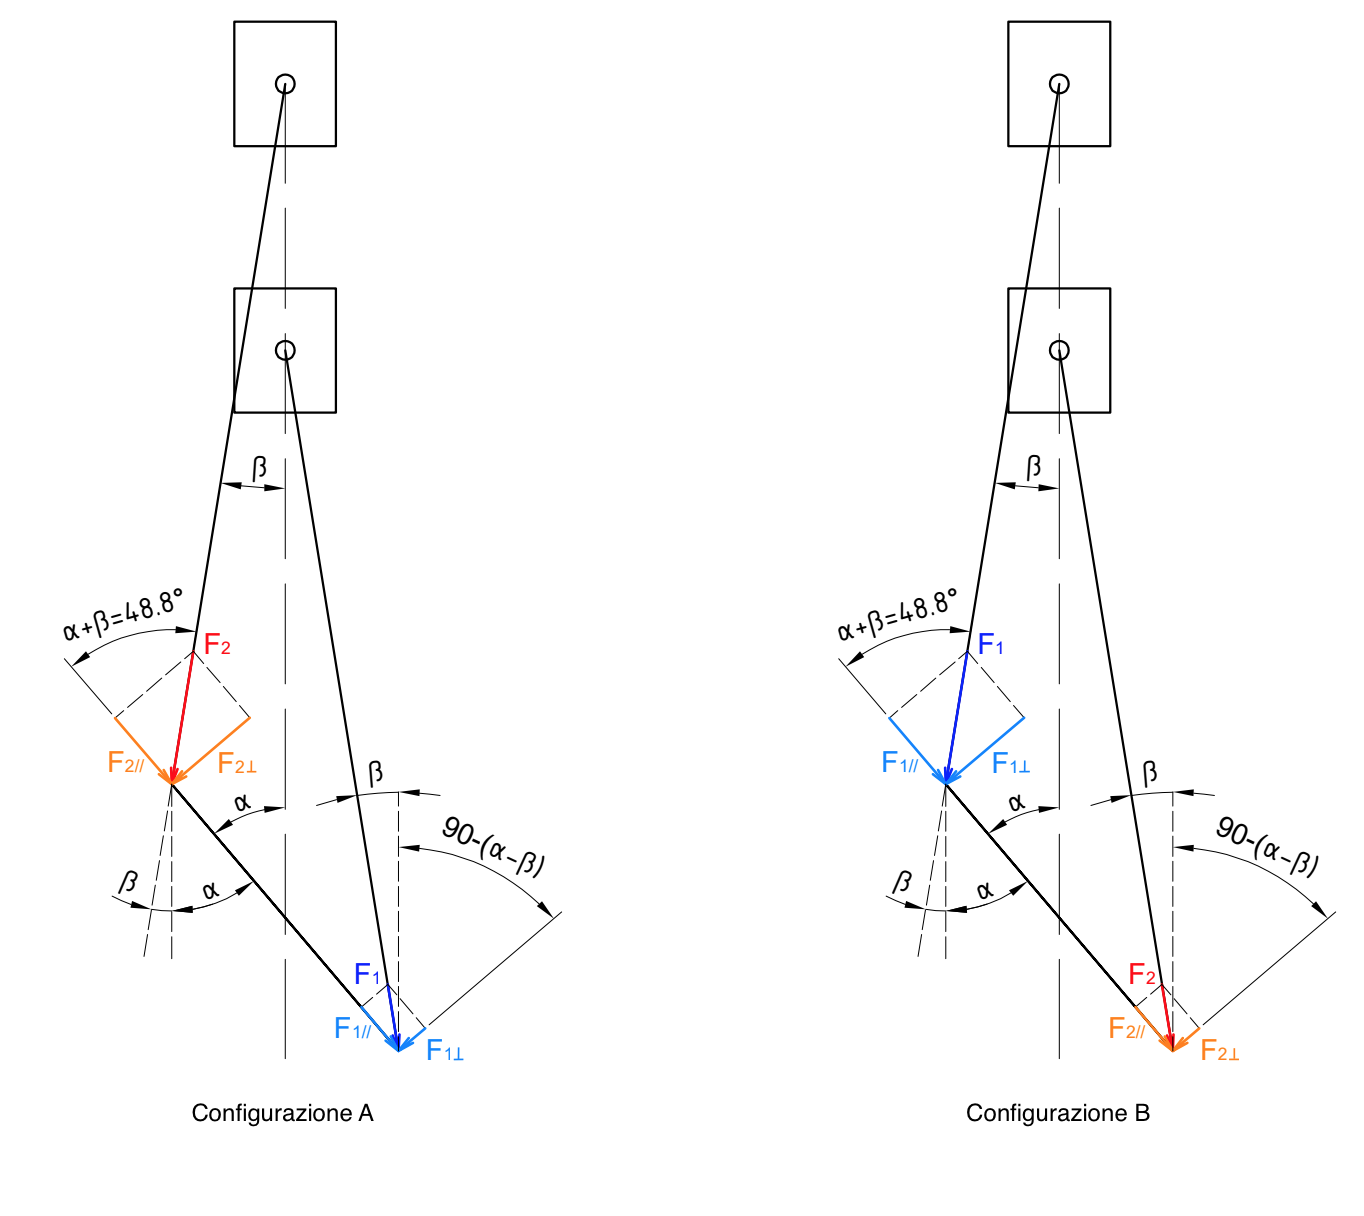
\includegraphics[scale=0.45]{Immagini/ScomposizioneForzeAlbero.png}
    \caption{Scomposizione delle due componenti della forza agente sull'albero a gomito}
    \label{fig:ScomposizioneForzeAlbero}
\end{figure}
Quando le manovelle sono soggette alla forza massima, le due componenti avranno valore:
\begin{itemize}
    \item $F_{\parallel}=F_{max}\cdot \sin \gamma=2500\cdot \sin (41,2°)= 1646\ N$
    \item $F_{\perp}=F_{max}\cdot\cos\gamma=2500\cdot \cos(41,2°)=1881\ N$
\end{itemize}
dove $\gamma=\frac{\pi}{2}-\left(\beta+\alpha\right)$.
\newpage
\subsubsection{Andamento delle caratteristiche di sollecitazione}
È possibile studiare questo componente mediante un modello a trave di Scienza delle Costruzioni. 
\paragraph{Configurazione A, piano parallelo}
In questa situazione si avrà una schematizzazione come rappresentata di Fig.\ref{fig:SchemaAlberoAPar}.
\begin{figure}[h]
    \centering
    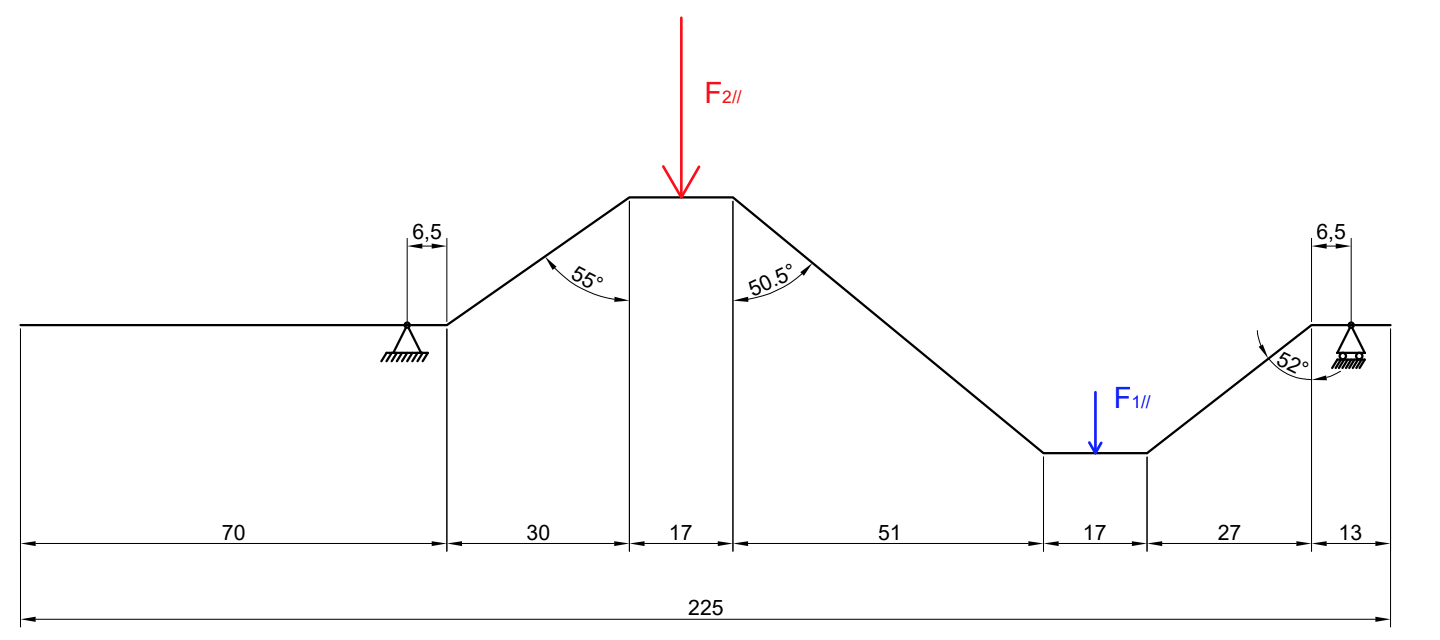
\includegraphics[scale=0.5]{Immagini/SchemaAlberoAPar.png}
    \caption{Configurazione A piano parallelo schematizzazione a trave albero a gomiti}
    \label{fig:SchemaAlberoAPar}
\end{figure}

Mediante software FTool è stato possibile valutare gli andamenti di taglio, momento flettente e sforzo normale. 
\newpage
\begin{figure}[h]
    \centering
    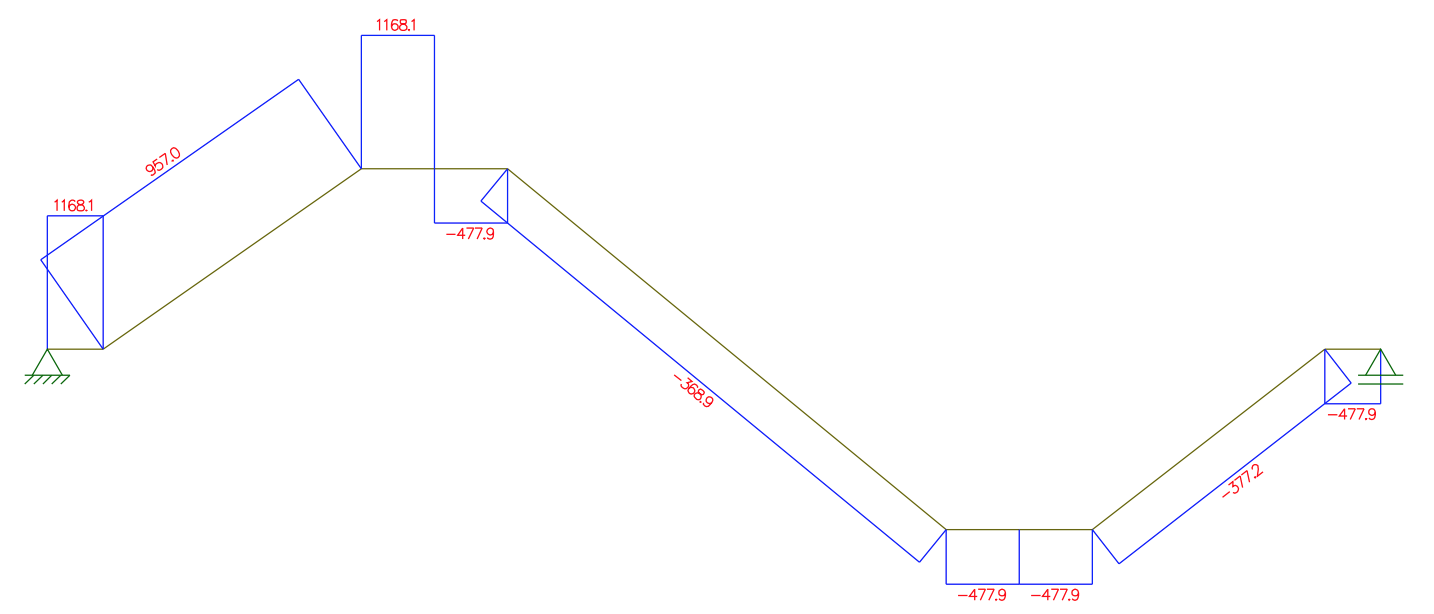
\includegraphics[scale=0.5]{Immagini/AndamentoTaglioAAlberoPar.png}
    \caption{Andamento dello sforzo di taglio in configurazione A, piano parallelo}
    \label{fig:AndamentoTalioAAlberoPar}
\end{figure}
\begin{figure}[h]
    \centering
    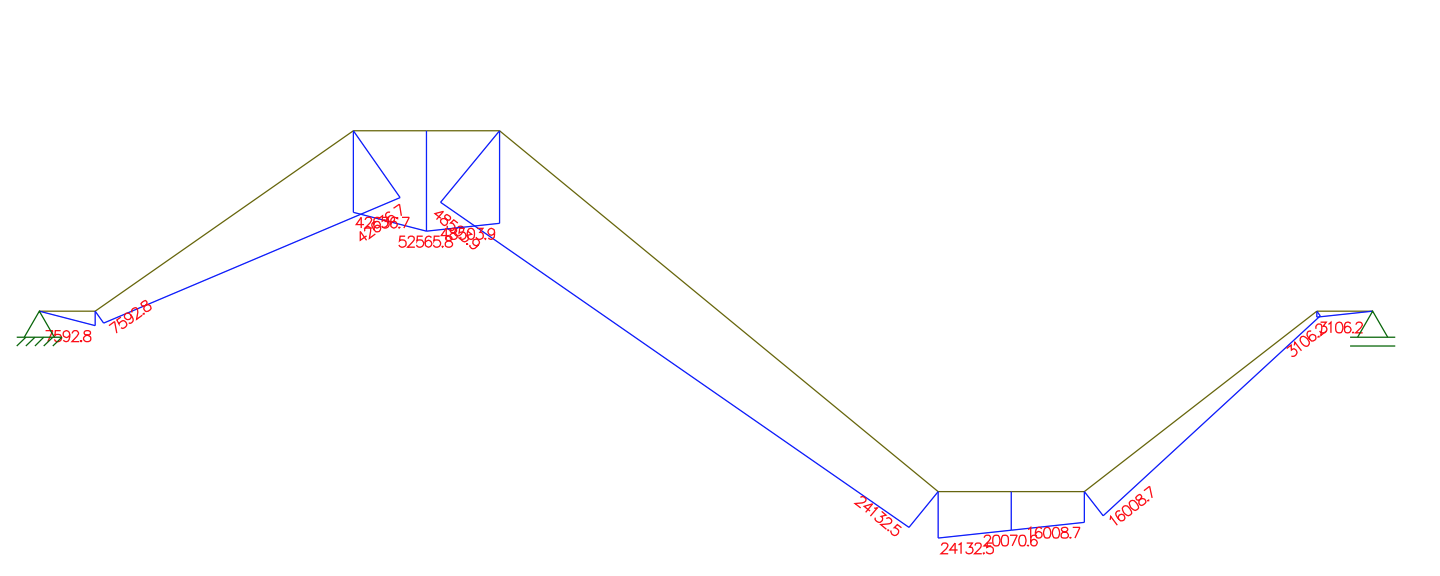
\includegraphics[scale=0.5]{Immagini/AndamentoMomentoAAlberoPar.png}
    \caption{Andamento del momento flettente in configurazione A, piano parallelo}
    \label{fig:AndamentoMomentoAAlberoPar}
\end{figure}
\begin{figure}[h!]
    \centering
    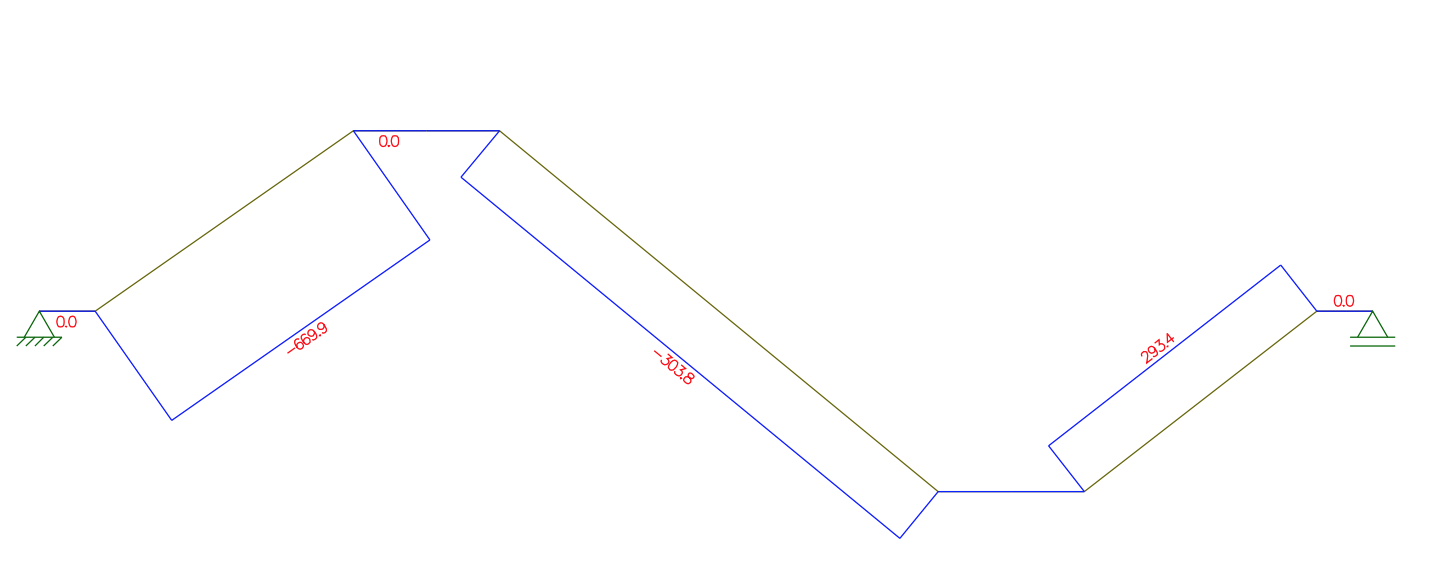
\includegraphics[scale=0.5]{Immagini/AndamentoNormaleAAlberoPar.png}
    \caption{Andamento dello sforzo normale in configurazione A, piano parallelo}
    \label{fig:AndamentoNormaleAAlberoPar}
\end{figure}
\newpage
\paragraph{Configurazione A, piano perpendicolare}
In questa situazione si avrà una schematizzazione come rappresentata di Fig.\ref{fig:SchemaAlberoAPerp}.
\begin{figure}[h]
    \centering
    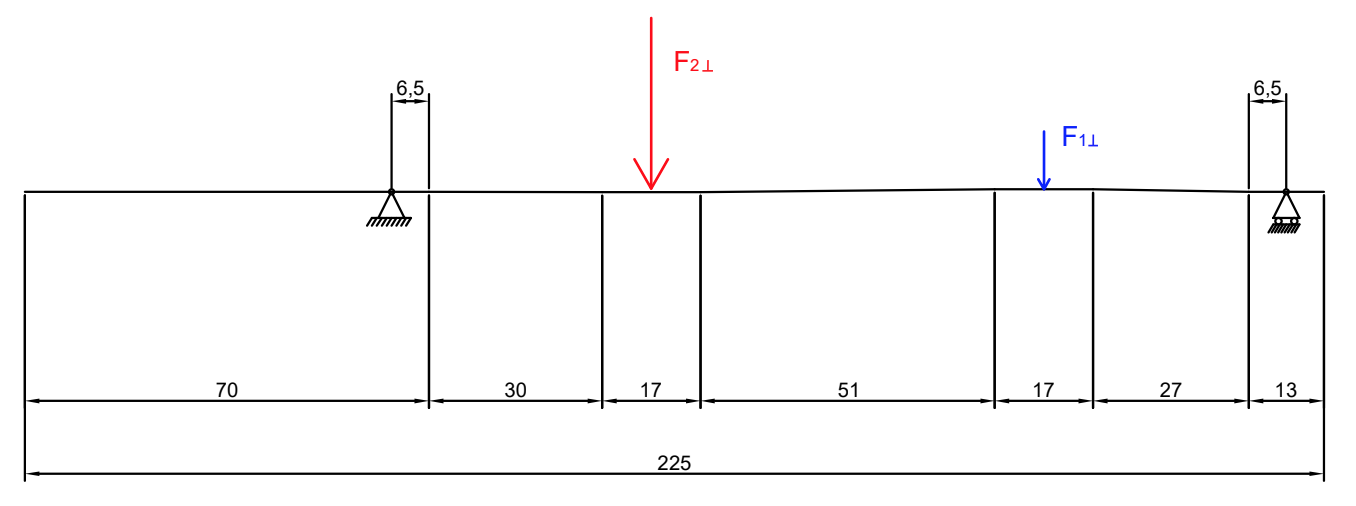
\includegraphics[scale=0.5]{Immagini/SchemaAlberoAPerp.png}
    \caption{Configurazione A piano perpendicolare schematizzazione a trave albero a gomiti}
    \label{fig:SchemaAlberoAPerp}
\end{figure}

Mediante software FTool è stato possibile valutare gli andamenti di taglio e momento flettente. 
\begin{figure}[h]
    \centering
    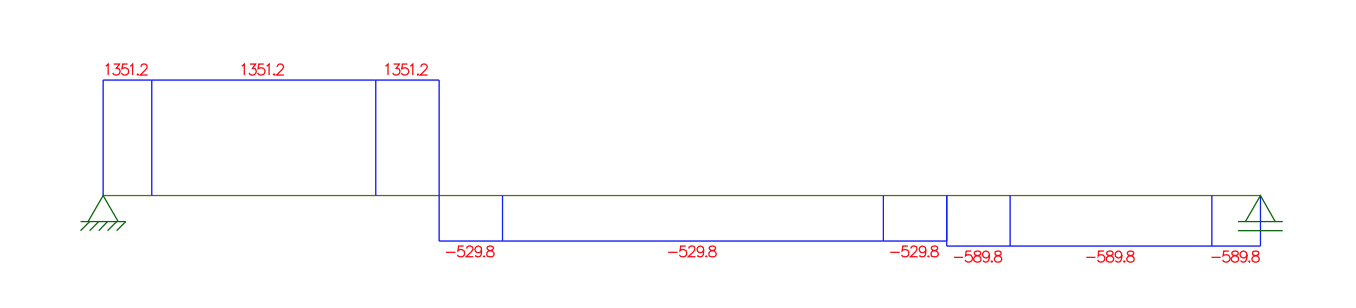
\includegraphics[scale=0.5]{Immagini/AndamentoTaglioAAlberoPerp.png}
    \caption{Andamento dello sforzo di taglio in configurazione A, piano perpendicolare}
    \label{fig:AndamentoTalioAAlberoPerp}
\end{figure}
\begin{figure}[h]
    \centering
    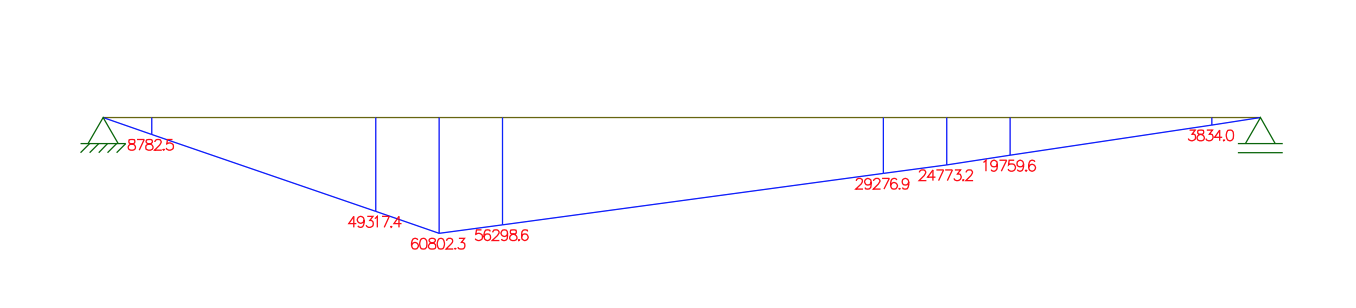
\includegraphics[scale=0.5]{Immagini/AndamentoMomentoAAlberoPerp.png}
    \caption{Andamento del momento flettente in configurazione A, piano perpendicolare}
    \label{fig:AndamentoMomentoAAlberoPerp}
\end{figure}
\newpage
\paragraph{Configurazione B, piano parallelo}
In questa situazione si avrà una schematizzazione come rappresentata di Fig.\ref{fig:SchemaAlberoBPar}.
\begin{figure}[h]
    \centering
    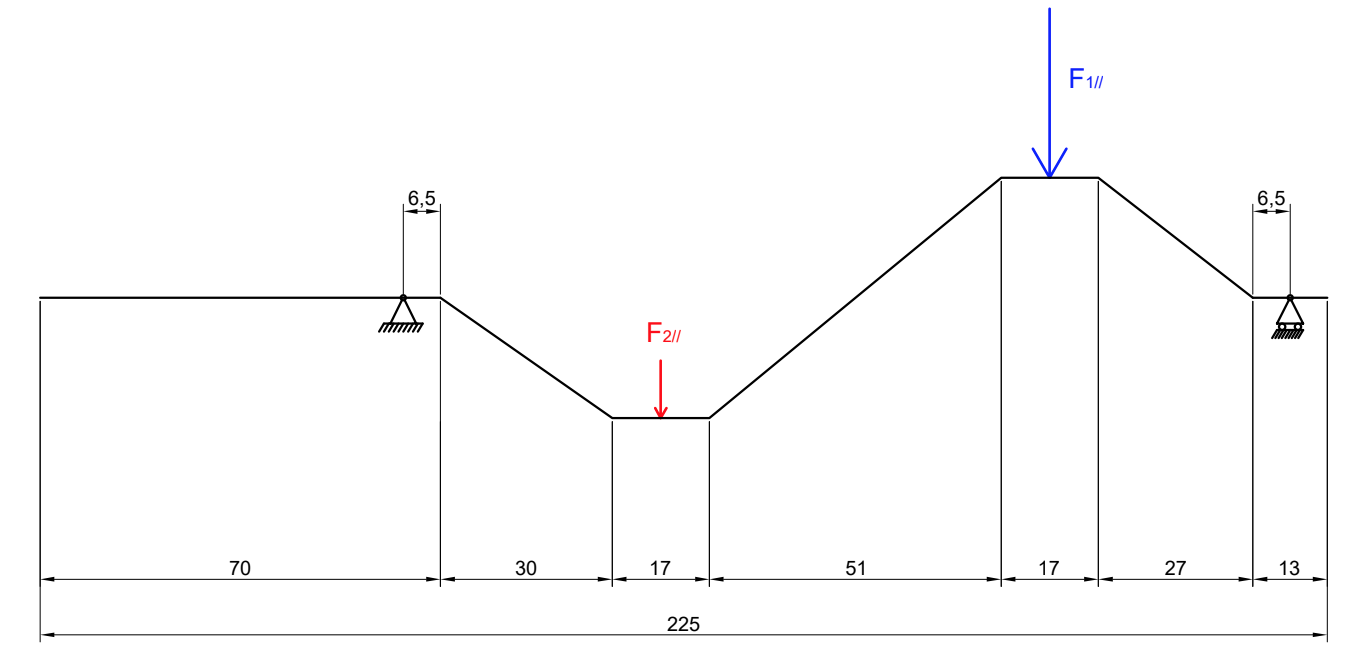
\includegraphics[scale=0.45]{Immagini/SchemaAlberoBPar.png}
    \caption{Configurazione B piano parallelo schematizzazione a trave albero a gomiti}
    \label{fig:SchemaAlberoBPar}
\end{figure}

Mediante software FTool è stato possibile valutare gli andamenti di taglio, momento flettente e sforzo normale. 
\begin{figure}[h]
    \centering
    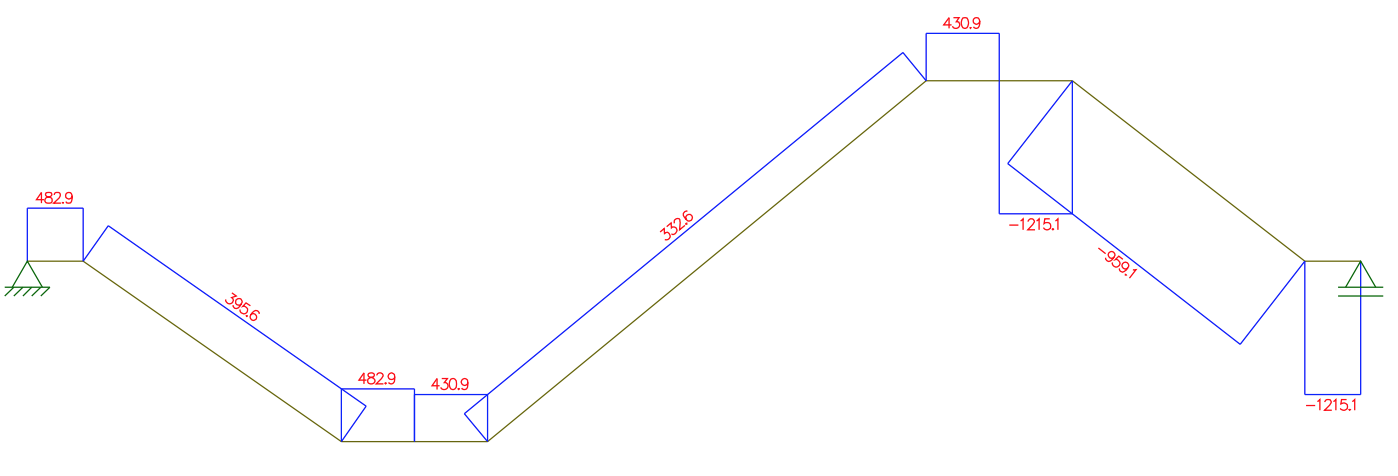
\includegraphics[scale=0.5]{Immagini/AndamentoTaglioBAlberoPar.png}
    \caption{Andamento dello sforzo di taglio in configurazione B, piano parallelo}
    \label{fig:AndamentoTalioBAlberoPar}
\end{figure}
\begin{figure}[h]
    \centering
    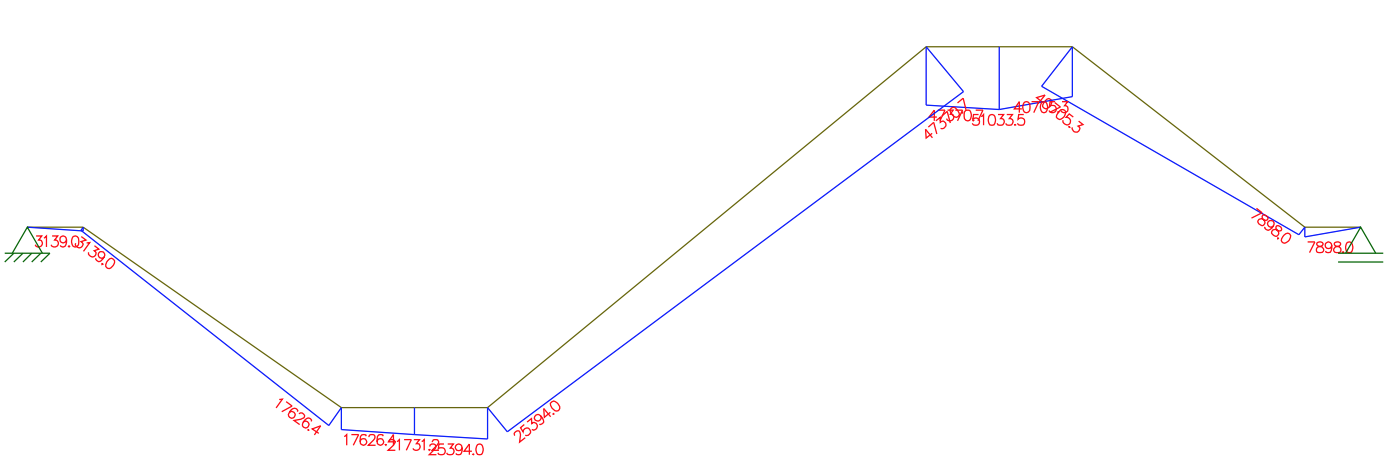
\includegraphics[scale=0.5]{Immagini/AndamentoMomentoBAlberoPar.png}
    \caption{Andamento del momento flettente in configurazione B, piano parallelo}
    \label{fig:AndamentoMomentoBAlberoPar}
\end{figure}
\begin{figure}[h]
    \centering
    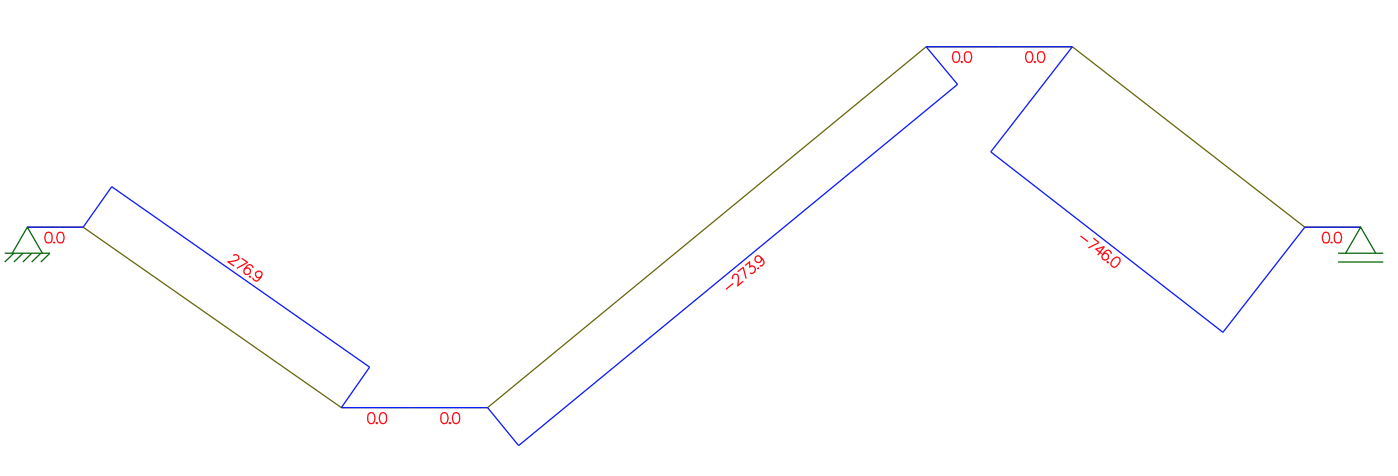
\includegraphics[scale=0.5]{Immagini/AndamentoNormaleBAlberoPar.png}
    \caption{Andamento dello sforzo normale in configurazione B, piano parallelo}
    \label{fig:AndamentoNormaleBAlberoPar}
\end{figure}
\newpage
\paragraph{Configurazione B, piano perpendicolare}
In questa situazione si avrà una schematizzazione come rappresentata di Fig.\ref{fig:SchemaAlberoBPerp}.
\begin{figure}[h]
    \centering
    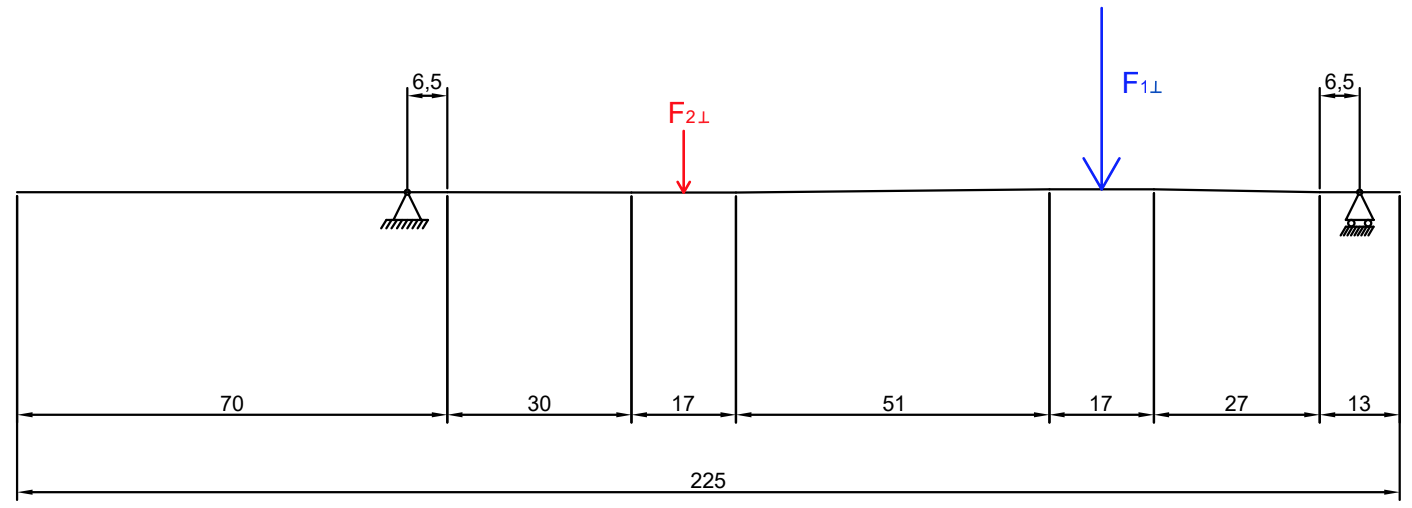
\includegraphics[scale=0.5]{Immagini/SchemaAlberoBPerp.png}
    \caption{Configurazione B piano perpendicolare schematizzazione a trave albero a gomiti}
    \label{fig:SchemaAlberoBPerp}
\end{figure}

Mediante software FTool è stato possibile valutare gli andamenti di taglio e momento flettente. 
\begin{figure}[h]
    \centering
    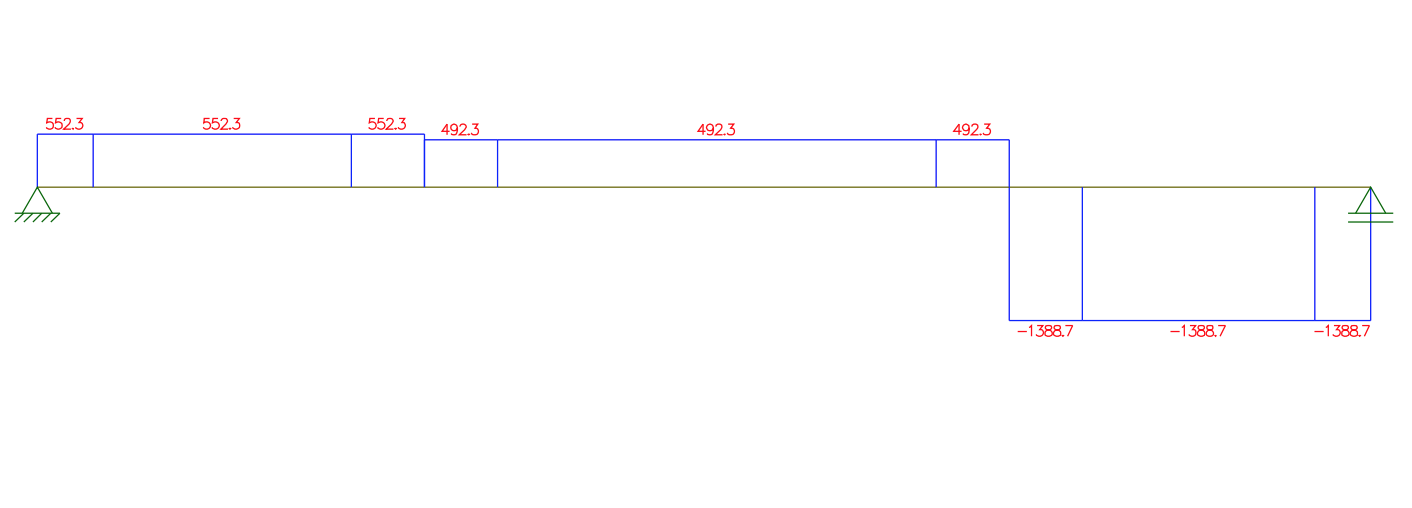
\includegraphics[scale=0.5]{Immagini/AndamentoTaglioBAlberoPerp.png}
    \caption{Andamento dello sforzo di taglio in configurazione B, piano perpendicolare}
    \label{fig:AndamentoTalioBAlberoPerp}
\end{figure}
\newpage
\begin{figure}[h]
    \centering
    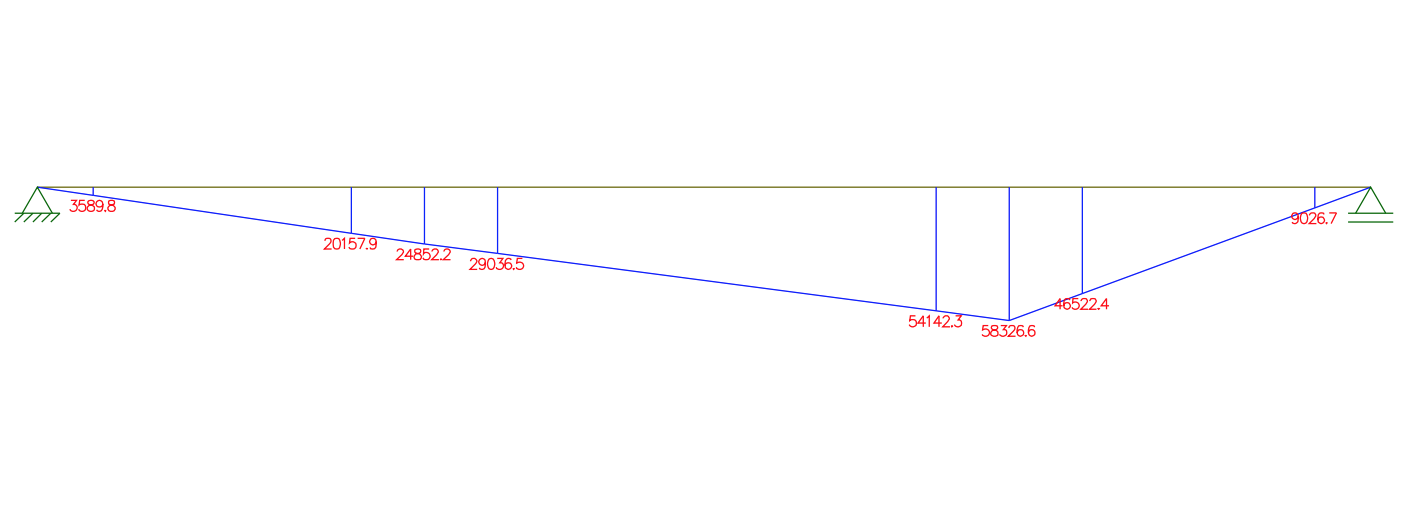
\includegraphics[scale=0.5]{Immagini/AndamentoMomentoBAlberoPerp.png}
    \caption{Andamento del momento flettente in configurazione B, piano perpendicolare}
    \label{fig:AndamentoMomentoBAlberoPerp}
\end{figure}
\subsubsection{Verifica statica}
In funzione della geometria e dell'andamento delle sollecitazioni agenti sull'albero a gomiti è possibile individuare quattro sezioni critiche.
\begin{figure}[h]
    \centering
    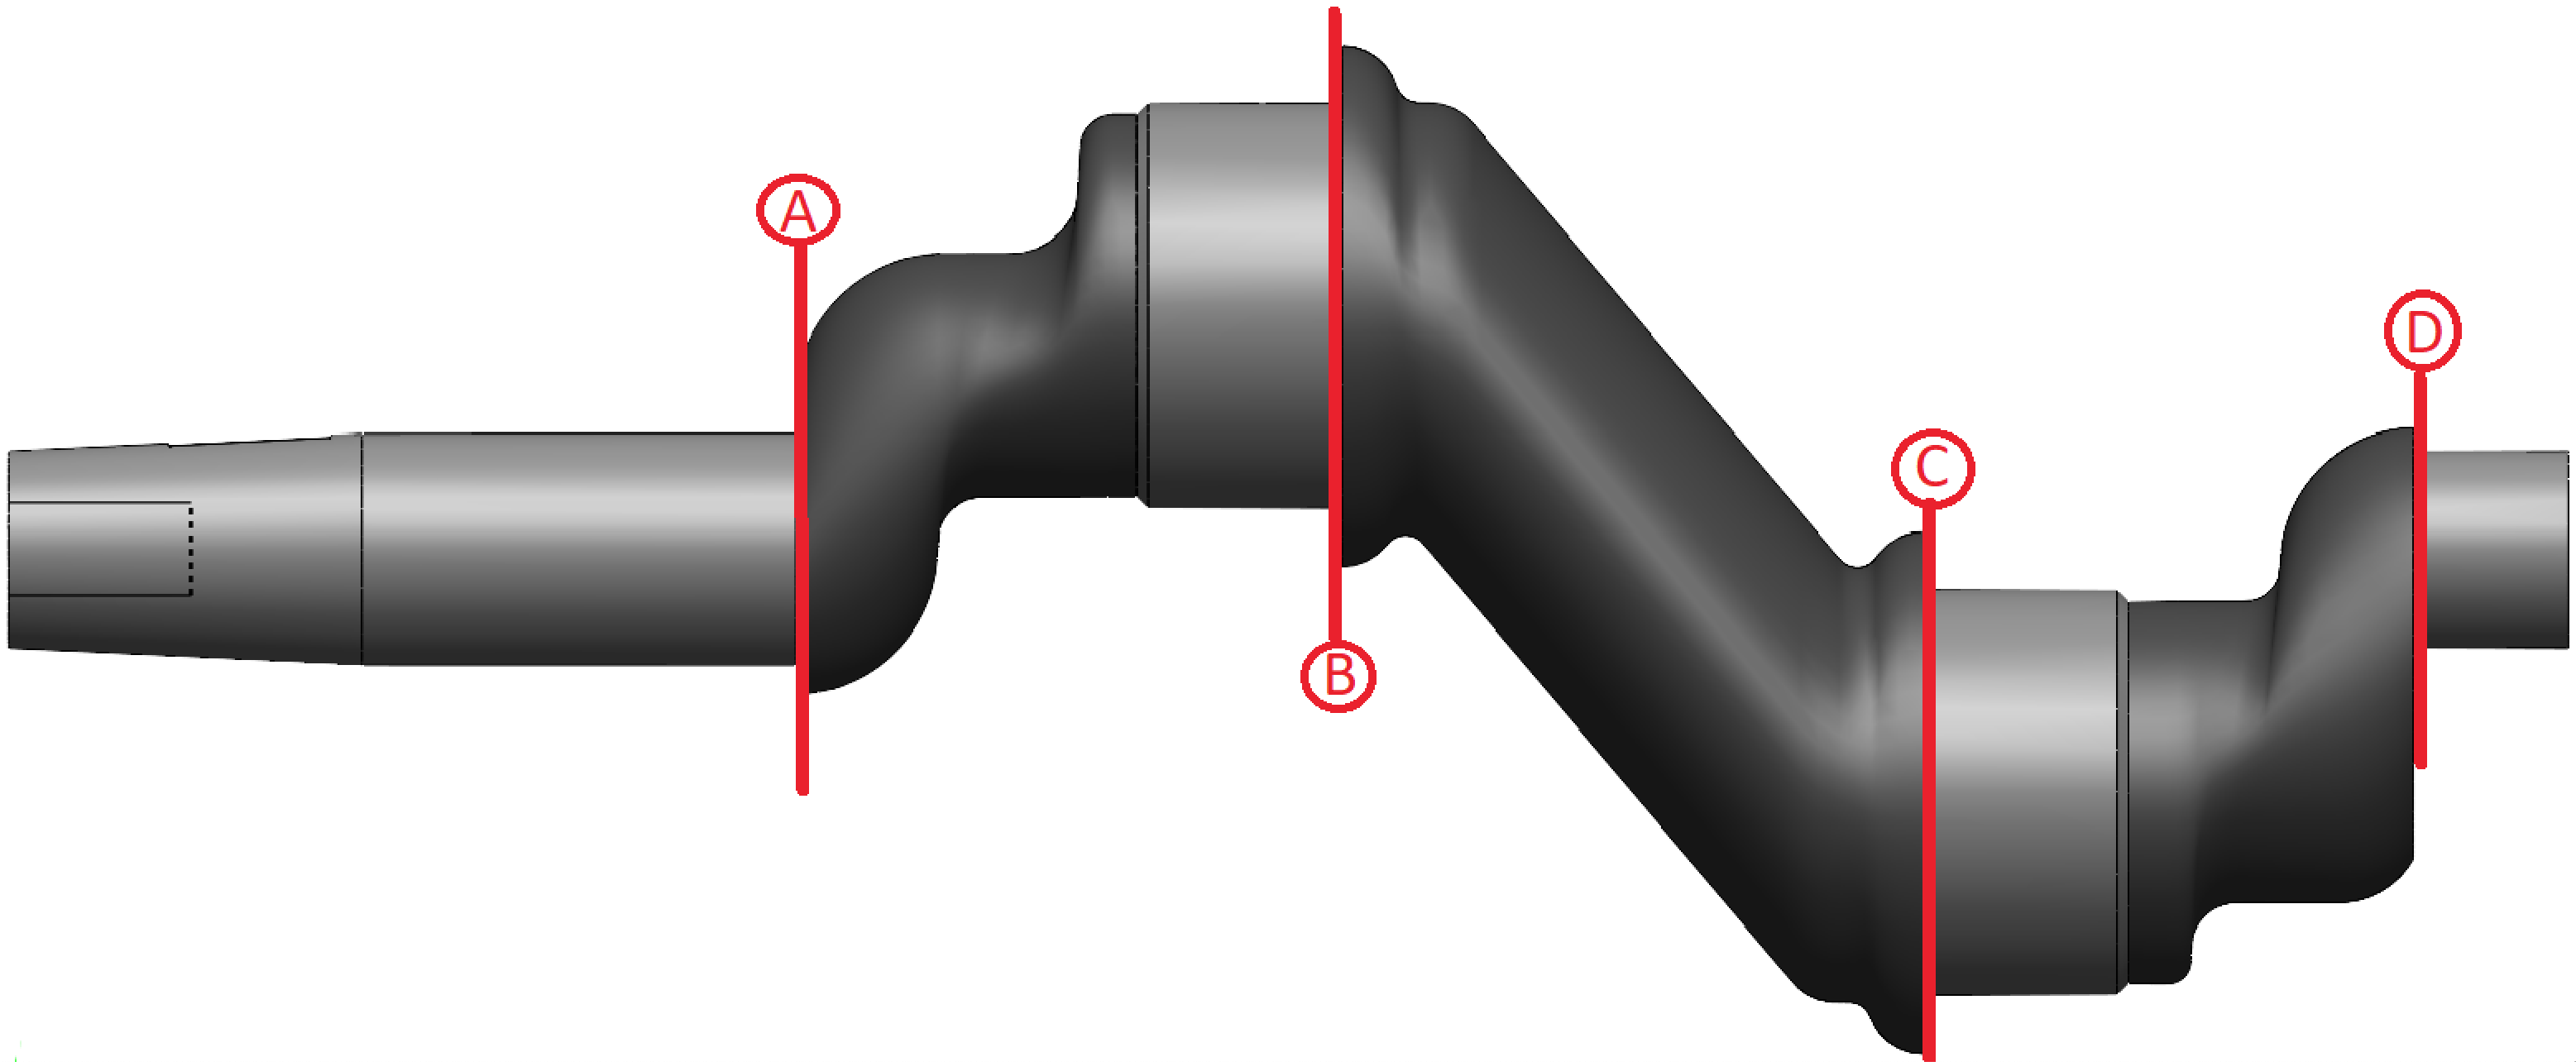
\includegraphics[scale=0.25]{Immagini/SezioniCriticheAlbero.png}
    \caption{Sezioni critiche individuate per l'albero a gomiti}
    \label{fig:SezioniCriticheAlbero}
\end{figure}

In configurazione A, la forza agente sulla manovella 1 è minima, quindi in tale configurazione le sezioni più sollecitate saranno la A e la B.\\
In configurazione B, la forza agente sulla manovella 2 è minima, quindi in tale configurazione le sezioni più sollecitate saranno la C e la D.\\
\\
\underline{\textbf{CONFIGURAZIONE A, SEZIONE A}}:
\paragraph{Sforzo normale} Dall'osservazione del diagramma delle caratteristiche di sollecitazione in Fig.\ref{fig:AndamentoNormaleAAlberoPar} è possibile calcolare la tensione nominale all'interno del componente mediante la formula:
\begin{equation}
    \sigma_{nom}=\frac{N}{A}=2,15\ MPa
\end{equation}
con $N=669\ N$ e $A=314,2\ mm^2$.\\
\\
Poiché in questa sezione è presente uno spallamento, si genererà un fenomeno di concentrazione delle tensioni valutabile attraverso l'introduzione del coefficiente $K_t=2,8$ ottenibile dal diagramma in Fig.\ref{fig:KtSpallamentoNormale}. 
\begin{figure}[h]
    \centering
    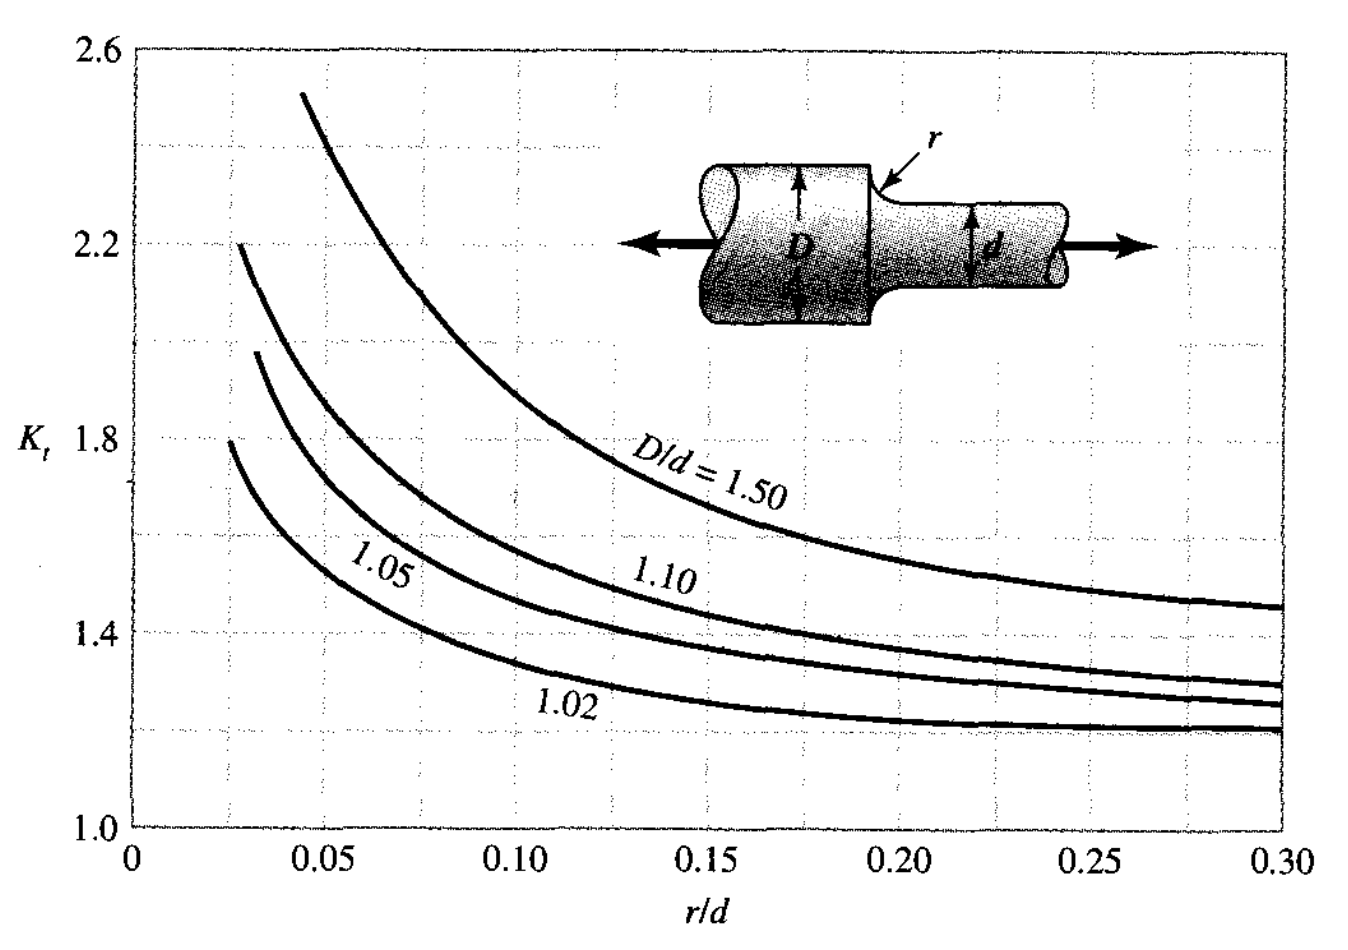
\includegraphics[scale=0.3]{Immagini/KtSpallementoNormale.png}
    \caption{Grafico del Kt per spallamento con sforzo normale}
    \label{fig:KtSpallamentoNormale}
\end{figure}
con $r/d=0,045$ e $D/d=1,5$.\\
Il raggio di raccordo per lo spallamento, è stato ipotizzato leggermente minore rispetto al raggio di raccordo della ralla interna del cuscinetto 6204, le cui caratteristica sono rappresentate in Fig.\ref{fig:Cuscinetto6204}.
\begin{figure}[h]
    \centering
    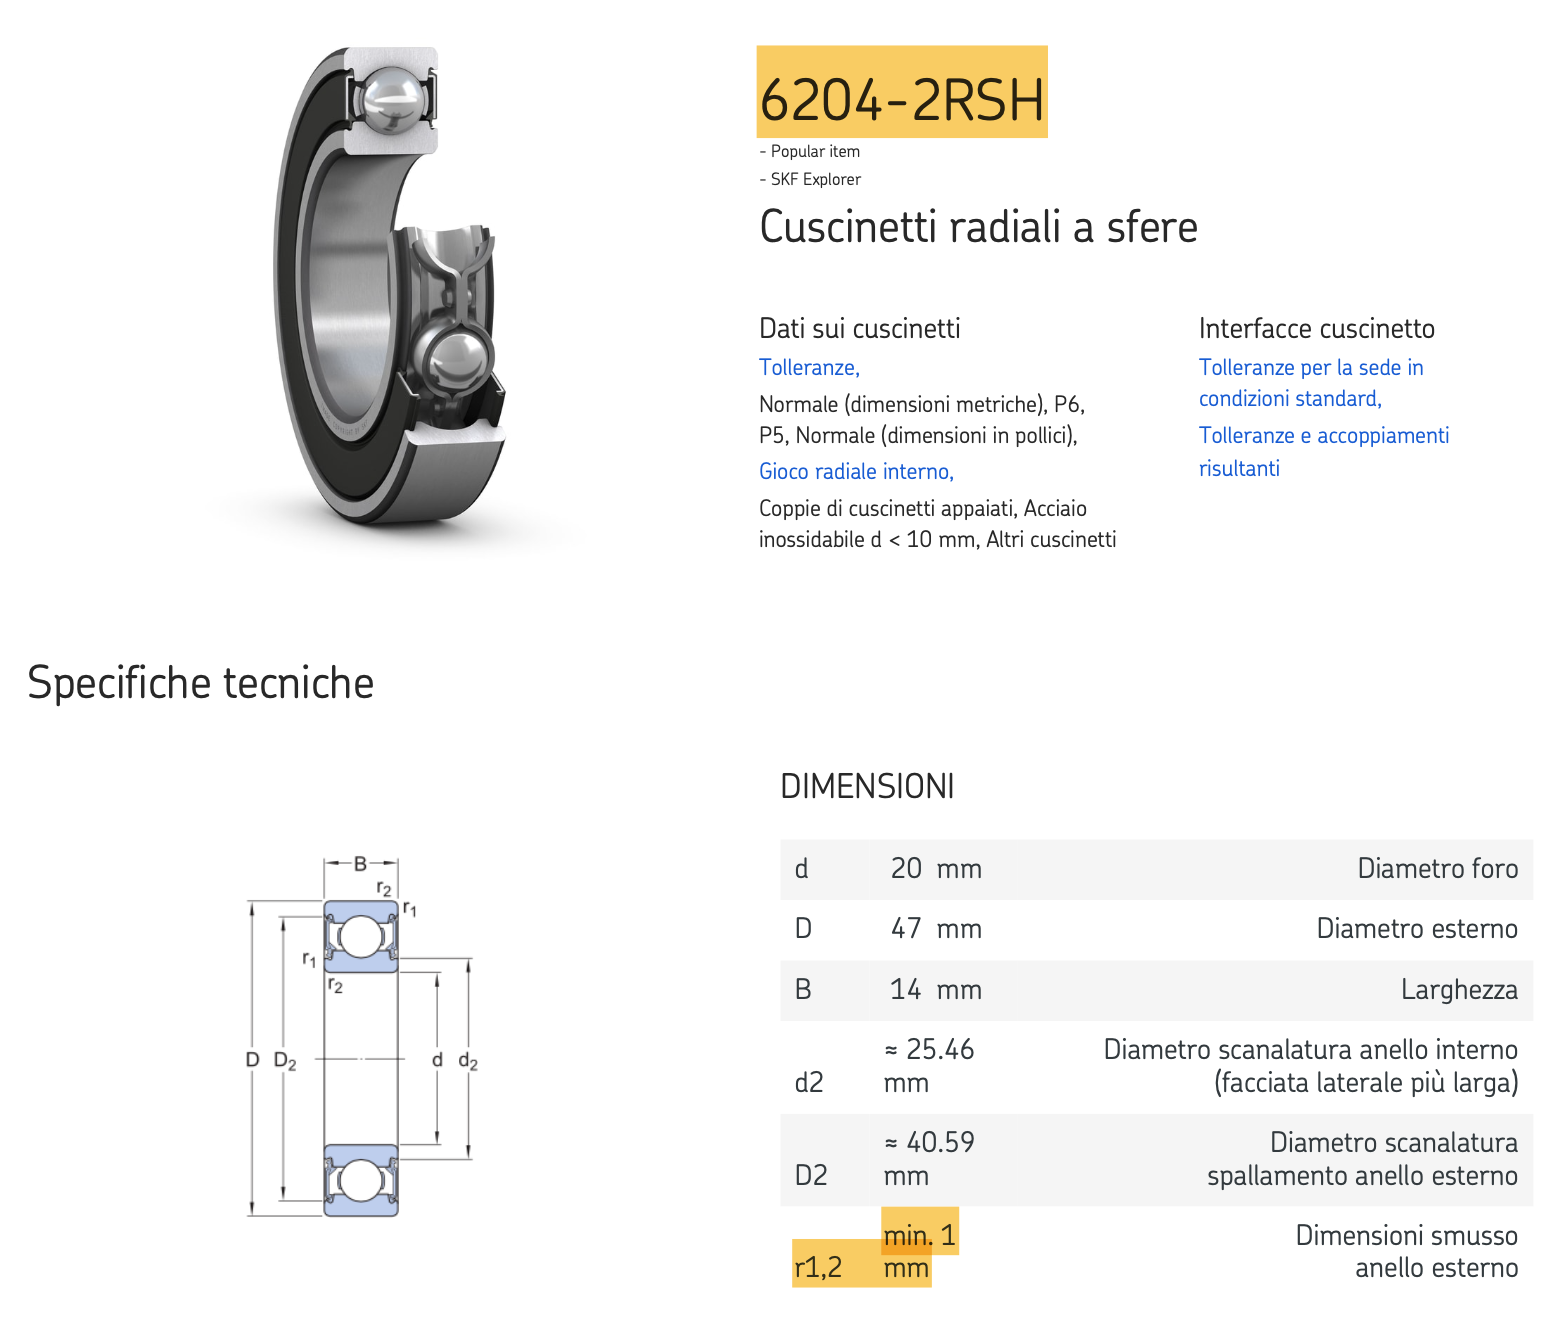
\includegraphics[scale=0.3]{Immagini/Cuscinetto6204.png}
    \caption{Cuscinetto 6204 da catalogo SKF}
    \label{fig:Cuscinetto6204}
\end{figure}

Si può quindi ricavare una tensione massima:
\begin{equation}
    \sigma_{max}=\sigma_{nom}\cdot K_t=6,02\ MPa.
\end{equation}
\paragraph{Sforzo dovuto al momento flettente}
Per la sezione circolare A è possibile calcolare il relativo modulo di resistenza a flessione mediante la formula:
\begin{equation}
    W=\frac{\pi d^3}{32}=785,4\ mm^3.
    \label{W_A}
\end{equation}
Attraverso i diagrammi delle caratteristiche di sollecitazione già osservate in Fig.\ref{fig:AndamentoMomentoAAlberoPar} e Fig.\ref{fig:AndamentoMomentoAAlberoPerp}, è possibile ricavare i valori dei due momenti flettenti agenti sui due piani ortogonali.\\ 
\\
Sommando i due contributi $M_{\parallel}=7684,4\ Nmm$ e $M_{\perp}=8782,5\ Nmm$ si ottiene un valore del momento flettente totale agente sulla sezione interessata pari a:
\begin{equation}
    M=\sqrt{M_{\parallel}^2+M_{\perp}^2}=11669,7\ Nmm.
\end{equation}

La tensione derivante da questo tipo di sforzo è ottenibile attraverso:
\begin{equation}
    \sigma_{nom}=\frac{M}{W}=14,85\ MPa.
\end{equation}
Analogamente a quanto considerato per lo sforzo normale, ci sarà da tenere conto di un fattore di intaglio che contempli concentrazioni di tensione sulla sezione. \\
Da Fig.\ref{fig:KtSpallamentoFlettente} è possibile estrapolare una valore di $K_t=2,4$ 
\begin{figure}[h]
    \centering
    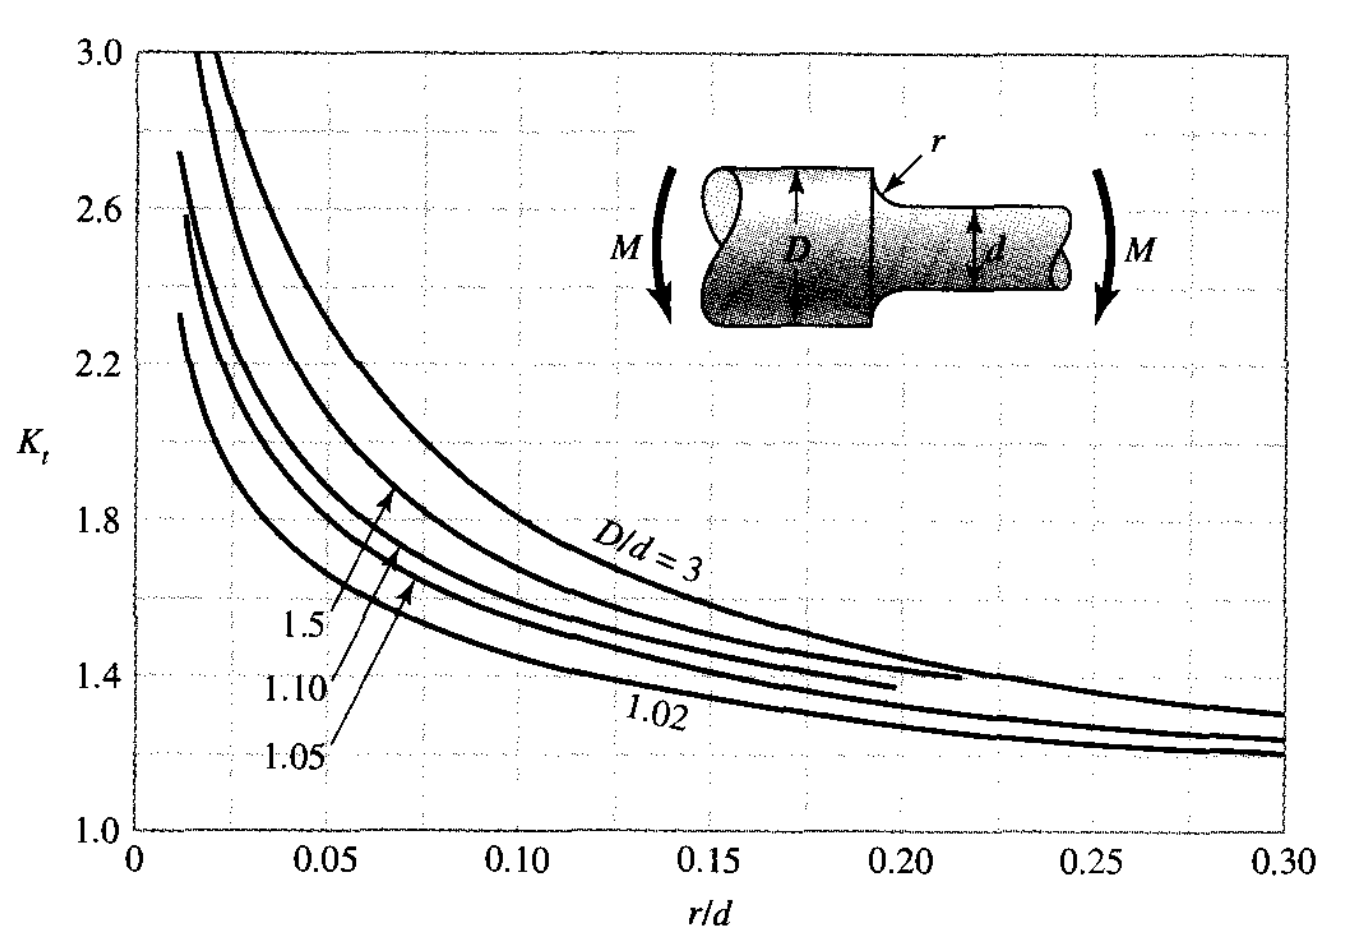
\includegraphics[scale=0.3]{Immagini/KtSpallamentoFlettente.png}
    \caption{Grafico del Kt per spallamento con sforzo a momento flettente}
    \label{fig:KtSpallamentoFlettente}
\end{figure}.

 da cui si ottiene una tensione massima di flessione:
 \begin{equation}
     \sigma_{max}=\sigma_{nom}\cdot K_t= 35,65\ MPa.
 \end{equation}
 
 La tensione \textbf{normale} massima raggiunta nella sezione A è data dalla somma dei due contributi normale e flessionale:
\begin{equation}
    \sigma_{tot}=\sigma_{Max,N}+\sigma_{Max,Mf}=41,7\ MPa.
\end{equation}
\paragraph{Sforzo di taglio}
 Attraverso i diagrammi delle caratteristiche di sollecitazione già osservate in Fig.\ref{fig:AndamentoTalioAAlberoPar} e Fig.\ref{fig:AndamentoTalioAAlberoPerp}, è possibile ricavare i valori dei due sforzi di taglio agenti sui due piani ortogonali.\\ 
Sommando i due contributi $V_{\parallel}=1182,2\ N$ e $V_{\perp}=1351,2\ N$ si ottiene un valore dello sforzo di taglio totale agente sulla sezione interessata pari a:
\begin{equation}
    V=\sqrt{V_{\parallel}^2+V_{\perp}^2}=1795,4\ N.
\end{equation}
La tensione dovuta a questo tipo di sforzo è calcolabile mediante:
\begin{equation}
    \tau=\frac{V}{A}=5,71\ MPa.
    \label{tauTaglioA}
\end{equation}
\paragraph{Sforzo torcente}Per la sezione circolare A è possibile calcolare il relativo modulo di resistenza polare a torsione mediante la formula:
\begin{equation}
    W_p=\frac{\pi d^3}{16}=1570,8\ mm^3.
\end{equation}
Dalla Fig.\ref{fig:GraficoMomentoTotale} il momento torcente massimo agente sull'albero a gomiti è pari a $M_t=36516,7\ Nmm$. \\
Nonostante la presenza di un volano che regolarizza tale andamento, si è scelto comunque di considerare il picco del grafico per adottare un approccio più cautelativo.\\
La tensione derivante da questa sollecitazione è ottenibile attraverso:
\begin{equation}
    \tau=\frac{Mt}{W_p}=23,24\ MPa
    \label{tauATorcente}
\end{equation}
 La tensione \textbf{tangenziale} massima raggiunta nella sezione A è data dalla somma dei due contributi di taglio e torsione:
\begin{equation}
    \tau_{tot}=\tau_{V}+\tau_{M_t}=28,95\ MPa.
\end{equation}

Si procede ora alla verifica statica seguendo il criterio di Von Mises:
\begin{equation}
    \sigma_{eq}=\sqrt{\sigma_{tot}^2+3\tau_{tot}^2}=61,5\ MPa
\end{equation}
considerando una $\sigma_{amm}=500\ MPa$, si ottiene un coefficiente di sicurezza pari a:
\begin{equation}
    n=\frac{\sigma_{amm}}{\sigma_{eq}}=8,1
\end{equation}
la sezione risulta quindi verificata staticamente.\\
\\
\underline{\textbf{CONFIGURAZIONE A, SEZIONE B}}:
\paragraph{Sforzo normale} Dall'osservazione del diagramma delle caratteristiche di sollecitazione in Fig.\ref{fig:AndamentoNormaleAAlberoPar} si deduce che su questa sezione non agisce alcun sforzo normale.
\paragraph{Sforzo dovuto a momento flettente} Per la sezione circolare B è possibile calcolare il relativo modulo di resistenza a flessione mediante la formula:
\begin{equation}
    W=\frac{\pi d^3}{32}=4209,2\ mm^3.
    \label{W_B}
\end{equation}
Attraverso i diagrammi delle caratteristiche di sollecitazione già osservate in Fig.\ref{fig:AndamentoMomentoAAlberoPar} e Fig.\ref{fig:AndamentoMomentoAAlberoPerp}, è possibile ricavare i valori dei due momenti flettenti agenti sui due piani ortogonali.\\ 
Sommando i due contributi $M_{\parallel}=53199,9\ Nmm$ e $M_{\perp}=60802,3\ Nmm$ si ottiene un valore del momento flettente totale agente sulla sezione interessata pari a:
\begin{equation}
    M=\sqrt{M_{\parallel}^2+M_{\perp}^2}=80790,7\ Nmm.
\end{equation}

La tensione derivante da questo tipo di sforzo è ottenibile attraverso:
\begin{equation}
    \sigma_{nom}=\frac{M}{W}=19,2\ MPa
\end{equation}
sarà necessario tenere conto di un fattore di intaglio che contempli concentrazioni di tensione sulla sezione. \\
Da Fig.\ref{fig:KtSpallamentoFlettente} è possibile estrapolare una valore di $K_t=2,3$, con $r/d=0,03$ e $D/d=1,2$. \\
Da cui si ottiene una tensione massima di flessione:
 \begin{equation}
     \sigma_{Max}=\sigma_{nom}\cdot K_t= 44,16\ MPa.
 \end{equation}
 \paragraph{Sforzo di taglio}
 Attraverso i diagrammi delle caratteristiche di sollecitazione già osservate in Fig.\ref{fig:AndamentoTalioAAlberoPar} e Fig.\ref{fig:AndamentoTalioAAlberoPerp}, è possibile ricavare i valori dei due sforzi di taglio agenti sui due piani ortogonali.\\ 
Sommando i due contributi $V_{\parallel}=1182,2\ N$ e $V_{\perp}=1351,2\ N$ si ottiene un valore dello sforzo di taglio totale agente sulla sezione interessata pari a:
\begin{equation}
    V=\sqrt{V_{\parallel}^2+V_{\perp}^2}=1795,4\ N.
\end{equation}
La tensione dovuta a questo tipo di sforzo è calcolabile mediante:
\begin{equation}
    \tau=\frac{V}{A}=1,9\ MPa.
\end{equation}

Si procede ora alla verifica statica seguendo il criterio di Von Mises:
\begin{equation}
    \sigma_{eq}=\sqrt{\sigma_{Max}^2+3\tau^2}=44,28\ MPa
\end{equation}
considerando una $\sigma_{amm}=500\ MPa$ si ottiene un coefficiente di sicurezza pari a:
\begin{equation}
    n=\frac{\sigma_{amm}}{\sigma_{eq}}=11,3
\end{equation}
la sezione risulta verificata staticamente.\\
\\
\underline{\textbf{CONFIGURAZIONE B, SEZIONE D}}:
\paragraph{Sforzo normale} Dall'osservazione del diagramma delle caratteristiche di sollecitazione in Fig.\ref{fig:AndamentoNormaleBAlberoPar} è possibile calcolare la tensione nominale all'interno del componente mediante la formula:
\begin{equation}
    \sigma_{nom}=\frac{N}{A}=3,3\ MPa
\end{equation}
con $N=746\ N$ e $A=226,9\ mm^2$.\\
\\
Poiché in questa sezione è presente uno spallamento, si genererà un fenomeno di concentrazione delle tensioni valutabile attraverso l'introduzione del coefficiente $K_t=2,8$ ottenibile dal diagramma in Fig.\ref{fig:KtSpallamentoNormale} ($r/d=0,06$ e $D/d=1,7$).\\
A differenza di quanto considerato per la sezione A, in prossimità dello spallamento è presente un distanziale, che consente di evitare lo strisciamento tra la ralla esterna del cuscinetto e lo spallamento stesso. In questo modo inoltre, si ha la possibilità di svincolarsi dalla necessità di adottare un raggio di raccordo inferiore rispetto a quello che presenterebbe la ralla interna del cuscinetto 6203. \\
Si può quindi ricavare una tensione massima:
\begin{equation}
    \sigma_{max}=\sigma_{nom}\cdot K_t=9,24\ MPa.
\end{equation}
\paragraph{Sforzo dovuto al momento flettente}
Per la sezione circolare D è possibile calcolare il relativo modulo di resistenza a flessione mediante la formula:
\begin{equation}
    W=\frac{\pi d^3}{32}=482,3\ mm^3.
    \label{W_D}
\end{equation}
Attraverso i diagrammi delle caratteristiche di sollecitazione già osservate in Fig.\ref{fig:AndamentoMomentoBAlberoPar} e Fig.\ref{fig:AndamentoMomentoBAlberoPerp}, è possibile ricavare i valori dei due momenti flettenti agenti sui due piani ortogonali.\\ 
Sommando i due contributi $M_{\parallel}=7898\ Nmm$ e $M_{\perp}=9026,7\ Nmm$ si ottiene un valore del momento flettente totale agente sulla sezione interessata pari a:
\begin{equation}
    M=\sqrt{M_{\parallel}^2+M_{\perp}^2}=11994\ Nmm.
\end{equation}

La tensione derivante da questo tipo di sforzo è ottenibile attraverso:
\begin{equation}
    \sigma_{nom}=\frac{M}{W}=24,914,85\ MPa.
\end{equation}
Analogamente a quanto considerato per lo sforzo normale, ci sarà da tenere conto di un fattore di intaglio che contempli concentrazioni di tensione sulla sezione. \\
Da Fig.\ref{fig:KtSpallamentoFlettente} è possibile estrapolare una valore di $K_t=2$, da cui si ottiene una tensione massima di flessione:
 \begin{equation}
     \sigma_{max}=\sigma_{nom}\cdot K_t= 49,8\ MPa.
 \end{equation}
 
 La tensione \textbf{normale} massima raggiunta nella sezione D è data dalla somma dei due contributi normale e flessionale:
\begin{equation}
    \sigma_{tot}=\sigma_{Max,N}+\sigma_{Max,Mf}=59\ MPa.
\end{equation}
\paragraph{Sforzo di taglio}
 Attraverso i diagrammi delle caratteristiche di sollecitazione già osservate in Fig.\ref{fig:AndamentoTalioBAlberoPar} e Fig.\ref{fig:AndamentoTalioBAlberoPerp}, è possibile ricavare i valori dei due sforzi di taglio agenti sui due piani ortogonali.\\ 
Sommando i due contributi $V_{\parallel}=1215,1\ N$ e $V_{\perp}=1388,7\ N$ si ottiene un valore dello sforzo di taglio totale agente sulla sezione interessata pari a:
\begin{equation}
    V=\sqrt{V_{\parallel}^2+V_{\perp}^2}=1845,3\ N.
\end{equation}
La tensione dovuta a questo tipo di sforzo è calcolabile mediante:
\begin{equation}
    \tau=\frac{V}{A}=8,1\ MPa.
\end{equation}
\paragraph{Sforzo torcente}Per la sezione circolare D è possibile calcolare il relativo modulo di resistenza polare a torsione mediante la formula:
\begin{equation}
    W_p=\frac{\pi d^3}{16}=964,7\ mm^3.
\end{equation}
Dalla Fig.\ref{fig:GraficoMomentoTotale} il momento torcente massimo agente sull'albero a gomiti è pari a $M_t=36516,7\ Nmm$ (approccio più cautelativo).\\
La tensione derivante da questa sollecitazione è ottenibile attraverso:
\begin{equation}
    \tau=\frac{Mt}{W_p}=37,9\ MPa.
\end{equation}
 La tensione \textbf{tangenziale} massima raggiunta nella sezione D è data dalla somma dei due contributi di taglio e torsione:
\begin{equation}
    \tau_{tot}=\tau_{V}+\tau_{M_t}=46\ MPa.
\end{equation}

Si procede ora alla verifica statica seguendo il criterio di Von Mises:
\begin{equation}
    \sigma_{eq}=\sqrt{\sigma_{tot}^2+3\tau_{tot}^2}=99\ MPa
\end{equation}
considerando una $\sigma_{amm}=500\ MPa$, si ottiene un coefficiente di sicurezza pari a:
\begin{equation}
    n=\frac{\sigma_{amm}}{\sigma_{eq}}=5
\end{equation}
la sezione risulta quindi verificata staticamente.\\
\\
\underline{\textbf{CONFIGURAZIONE B, SEZIONE C}}:
\paragraph{Sforzo normale} Dall'osservazione del diagramma delle caratteristiche di sollecitazione in Fig.\ref{fig:AndamentoNormaleBAlberoPar} si deduce che su questa sezione non agisce alcun sforzo normale.
\paragraph{Sforzo dovuto a momento flettente} Per la sezione circolare C è possibile calcolare il relativo modulo di resistenza a flessione mediante la formula:
\begin{equation}
    W=\frac{\pi d^3}{32}=4209,2\ mm^3.
    \label{W_C}
\end{equation}
Attraverso i diagrammi delle caratteristiche di sollecitazione già osservate in Fig.\ref{fig:AndamentoMomentoBAlberoPar} e Fig.\ref{fig:AndamentoMomentoBAlberoPerp}, è possibile ricavare i valori dei due momenti flettenti agenti sui due piani ortogonali.\\ 
Sommando i due contributi $M_{\parallel}=51033,5\ Nmm$ e $M_{\perp}=58326,6\ Nmm$ si ottiene un valore del momento flettente totale agente sulla sezione interessata pari a:
\begin{equation}
    M=\sqrt{M_{\parallel}^2+M_{\perp}^2}=77501\ Nmm.
\end{equation}

La tensione derivante da questo tipo di sforzo è ottenibile attraverso:
\begin{equation}
    \sigma_{nom}=\frac{M}{W}=18,4\ MPa
\end{equation}
sarà necessario tenere conto di un fattore di intaglio che contempli concentrazioni di tensione sulla sezione. \\
Da Fig.\ref{fig:KtSpallamentoFlettente} è possibile estrapolare una valore di $K_t=2,3$, con $r/d=0,03$ e $D/d=1,2$. \\
Da cui si ottiene una tensione massima di flessione:
 \begin{equation}
     \sigma_{Max}=\sigma_{nom}\cdot K_t= 42,3\ MPa.
 \end{equation}
 \paragraph{Sforzo di taglio}
 Attraverso i diagrammi delle caratteristiche di sollecitazione già osservate in Fig.\ref{fig:AndamentoTalioBAlberoPar} e Fig.\ref{fig:AndamentoTalioBAlberoPerp}, è possibile ricavare i valori dei due sforzi di taglio agenti sui due piani ortogonali.\\ 
Sommando i due contributi $V_{\parallel}=1215,1\ N$ e $V_{\perp}=1388,7\ N$ si ottiene un valore dello sforzo di taglio totale agente sulla sezione interessata pari a:
\begin{equation}
    V=\sqrt{V_{\parallel}^2+V_{\perp}^2}=1845,3\ N.
\end{equation}
La tensione dovuta a questo tipo di sforzo è calcolabile mediante:
\begin{equation}
    \tau=\frac{V}{A}=1,9\ MPa.
\end{equation}

Si procede ora alla verifica statica seguendo il criterio di Von Mises:
\begin{equation}
    \sigma_{eq}=\sqrt{\sigma_{Max}^2+3\tau^2}=42,5\ MPa
\end{equation}
considerando una $\sigma_{amm}=500\ MPa$ si ottiene un coefficiente di sicurezza pari a:
\begin{equation}
    n=\frac{\sigma_{amm}}{\sigma_{eq}}=11,8
\end{equation}
la sezione risulta verificata staticamente.
\subsubsection{Verifica a fatica}
Mentre nella verifica statica venivano considerate soltanto le configurazioni tali per cui ciascuna sezione subiva lo sforzo massimo, nella fatica, essendo l'albero un componente rotante, risulta necessario considerare le medesime sezioni nominate in precedenza, in entrambe le configurazioni. \\
Tale approccio permette di evidenziare i di cicli carico delle sezioni durante il funzionamento del componente.\\
\\
\underline{\textbf{SEZIONE A}}:
\paragraph{Sforzo normale, configurazione A} Le tensioni nominali agenti in questa configurazione sono già state calcolate durante la verifica statica.\\
$\sigma_{nom}=2,15\ MPa$.
\paragraph{Sforzo dovuto a momento flettente, configurazione A} Le tensioni nominali agenti in questa configurazione sono già state calcolate durante la verifica statica.\\
$\sigma_{nom}=14,85\ MPa$.\\
\\
Quindi in questa configurazione la tensione nominale totale agente sarà pari a:
\begin{equation}
    \sigma_{nom,A}=\sigma_{nom,N}+\sigma_{nom,Mf}=17\ MPa
\end{equation}
\paragraph{Sforzo normale, configurazione B} Dall'osservazione del diagramma delle caratteristiche di sollecitazione in Fig.\ref{fig:AndamentoNormaleBAlberoPar} si deduce che su questa sezione agisce uno sforzo normale:\\
$\sigma_{nom}=\frac{N}{A_{min}}=\frac{276,9\ N}{314,2\ mm^2}=0,9\ MPa.$
\paragraph{Sforzo dovuto al momento flettente, configurazione B}Attraverso i diagrammi delle caratteristiche di sollecitazione già osservate in Fig.\ref{fig:AndamentoMomentoBAlberoPar} e Fig.\ref{fig:AndamentoMomentoBAlberoPerp}, è possibile ricavare i valori dei due momenti flettenti agenti sui due piani ortogonali.\\ 
Sommando i due contributi $M_{\parallel}=3139\ Nmm$ e $M_{\perp}=3589\ Nmm$ si ottiene un valore del momento flettente totale agente sulla sezione interessata pari a:
\begin{equation}
    M=\sqrt{M_{\parallel}^2+M_{\perp}^2}=4768\ Nmm.
\end{equation}
La tensione derivante da questo tipo di sforzo è ottenibile attraverso:
\begin{equation}
    \sigma_{nom}=\frac{M}{W}=6,1\ MPa
\end{equation}
con modulo di resistenza a flessione calcola in eq.(\ref{W_A}).\\
Quindi in questa configurazione la tensione nominale totale agente sarà pari a:
\begin{equation}
    \sigma_{nom,B}=\sigma_{nom,N}+\sigma_{nom,Mf}=7\ MPa
\end{equation}

Si ottiene da questi calcoli una variabilità delle tensioni da $\sigma_{max}$ a $\sigma_{min}$ in modo pressoché sinusoidale.\\
Ne risulta il seguente andamento del ciclo di carico:
\begin{figure}[h]
    \centering
    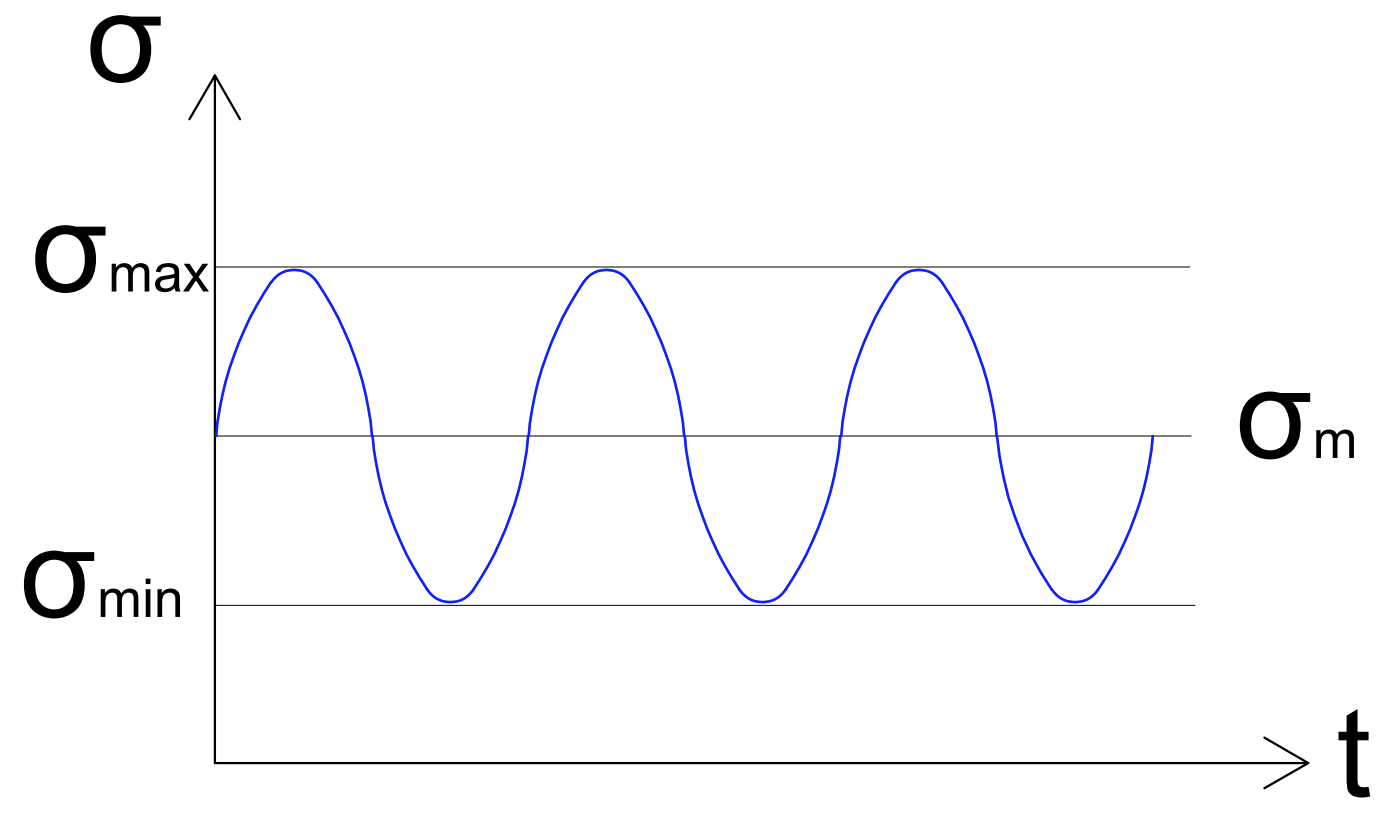
\includegraphics[scale=0.35]{Immagini/CicloFaticaANormale.png}
    \caption{Ciclo di carico normale sezione A}
    \label{fig:CicloFaticaANormale}
\end{figure}
\begin{itemize}
    \item $\sigma_{max}=\sigma_{nom,A}=17\ MPa$
    \item $\sigma_{min}=\sigma_{nom,B}=7\ MPa$
    \item $\sigma_m=\frac{\sigma_{max}+\sigma_{min}}{2}=12\ MPa$
    \item $\sigma_a=\sigma_{max}-\sigma_m=5\ MPa$
\end{itemize}
\paragraph{Sforzo torcente, configurazione A e B} La tensione tangenziale dovuta al momento torcente è uguale in entrambe le configurazioni, ed è già stata calcolata in eq.(\ref{tauATorcente}). 
\paragraph{Sforzo di taglio, configurazione A e B} In entrambe le configurazioni, la tensione tangenziale dovuta al taglio risulta ampiamente trascurabile rispetto alla tensione dovuta al momento torcente. \\
Ne risulta quindi il seguente andamento del ciclo di carico:
\newpage
\begin{figure}[h]
    \centering
    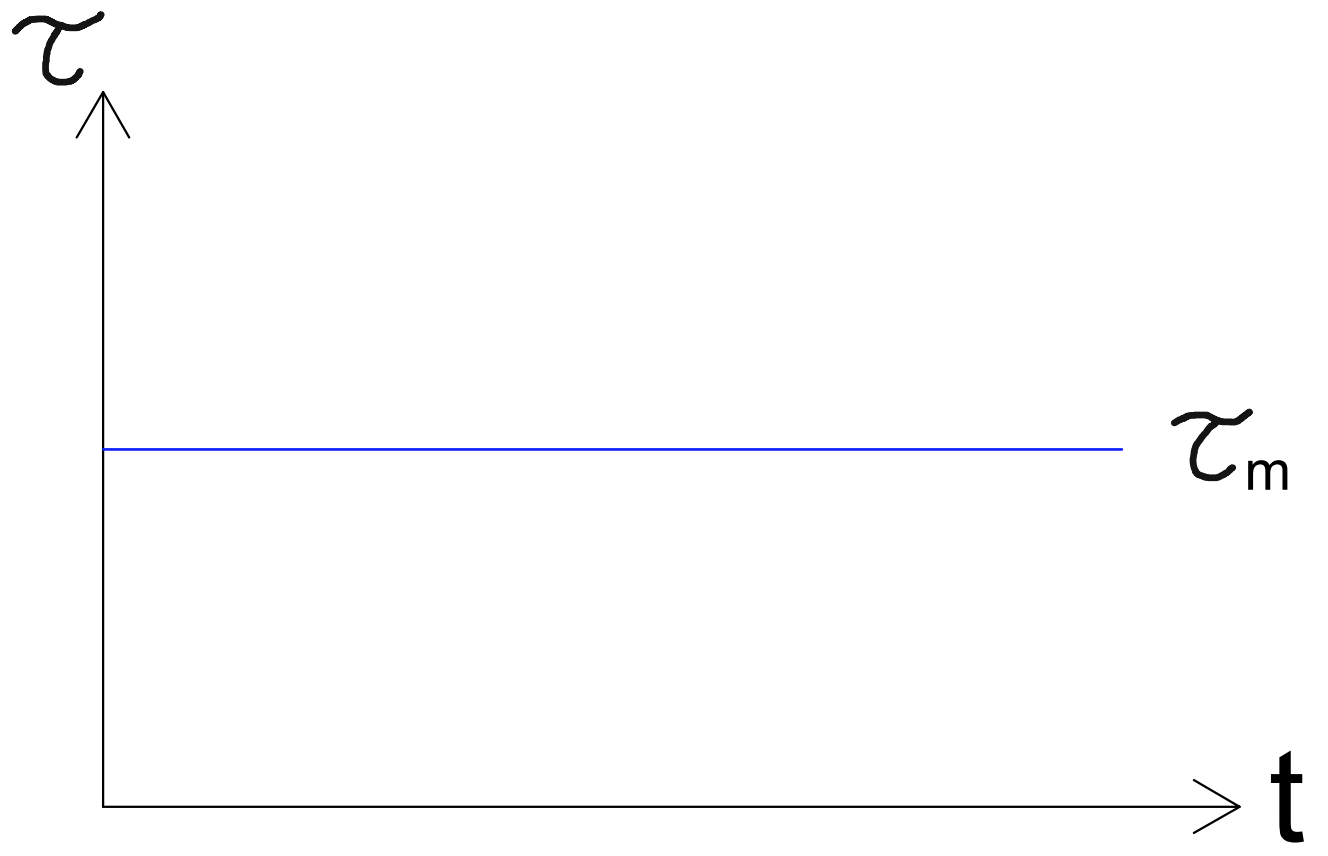
\includegraphics[scale=0.35]{Immagini/CicloFaticaATangenziale.png}
    \caption{Ciclo di carico tangenziale sezione A}
    \label{fig:CicloFaticaATangenziale}
\end{figure}
\begin{itemize}
    \item $\tau_m=\tau=23,24\ MPa$
\end{itemize}
È possibile ora stimare il limite di fatica con la seguente formula:
\begin{equation}
    \sigma_{w0}=0,5\cdot R_m\cdot C_{surf}\cdot C_{size}\cdot C_{load}=178\ MPa
\end{equation}
\begin{itemize}
    \item $C_{surf}=0,8$, da tabella in Fig.\ref{fig:CurvaCLoad} considerando rettifica 
    \item $C_{size}=1,189\cdot d^{-0,097}=0,89$
    \item $C_{load}=1$
\end{itemize}
Considerando il fattore di intaglio statico già calcolato, è possibile ottenere il fattore di intaglio a fatica
\begin{equation}
    K_f=q\left(K_t-1\right)+1=1,94
\end{equation}
dove $q=0,67$ ricavato mediante Fig.\ref{fig:KfBiella}.\\
In conclusione, si ottiene un coefficiente di sicurezza a fatica calcolato mediante:
\begin{equation}
    n=\sqrt{\frac{1}{\left(\frac{K_f\sigma_a}{\sigma_{w0}}\right)^2+\left(\frac{\tau_m}{\tau_s}\right)^2}}=7,3
\end{equation}
La sezione risulta quindi verificata a fatica. \\
\\
\underline{\textbf{SEZIONE B}}:
\paragraph{Sforzo normale, configurazione A} Dall'osservazione del diagramma delle caratteristiche di sollecitazione in Fig.\ref{fig:AndamentoNormaleAAlberoPar} si deduce che su questa sezione agisce uno sforzo normale:\\
$\sigma_{nom}=\frac{N}{A_{min}}=\frac{303.8\ N}{962.1\ mm^2}=0.32\ MPa$.
\paragraph{Sforzo dovuto a momento flettente, configurazione A} Le tensioni nominali agenti in questa configurazione sono già state calcolate durante la verifica statica.\\
$\sigma_{nom}=19,2\ MPa$.\\
\\
Quindi in questa configurazione la tensione nominale totale agente sarà pari a:
\begin{equation}
    \sigma_{nom,A}=\sigma_{nom,N}+\sigma_{nom,Mf}=19,52\ MPa
\end{equation}
\paragraph{Sforzo normale, configurazione B} Dall'osservazione del diagramma delle caratteristiche di sollecitazione in Fig.\ref{fig:AndamentoNormaleBAlberoPar} si deduce che agisce uno sforzo normale:\\
$\sigma_{nom}=\frac{N}{A_{min}}=\frac{273,9\ N}{962,1\ mm^2}=0,3\ MPa$.
\paragraph{Sforzo dovuto al momento flettente, configurazione B}Attraverso i diagrammi delle caratteristiche di sollecitazione già osservate in Fig.\ref{fig:AndamentoMomentoBAlberoPar} e Fig.\ref{fig:AndamentoMomentoBAlberoPerp}, è possibile ricavare i valori dei due momenti flettenti agenti sui due piani ortogonali.\\ 
Sommando i due contributi $M_{\parallel}=25394\ Nmm$ e $M_{\perp}=29036,5\ Nmm$ si ottiene un valore del momento flettente totale agente sulla sezione interessata pari a:
\begin{equation}
    M=\sqrt{M_{\parallel}^2+M_{\perp}^2}=38574,3\ Nmm.
\end{equation}
La tensione derivante da questo tipo di sforzo è ottenibile attraverso:
\begin{equation}
    \sigma_{nom}=\frac{M}{W}=9,2\ MPa
\end{equation}
con modulo di resistenza a flessione calcola in eq.(\ref{W_B}).\\
\\
Quindi in questa configurazione la tensione nominale totale agente sarà pari a:
\begin{equation}
    \sigma_{nom,B}=\sigma_{nom,N}+\sigma_{nom,Mf}=9,5\ MPa.
\end{equation}
Si ottiene da questi calcoli una variabilità delle tensioni da $\sigma_{max}$ a $\sigma_{min}$ in modo pressoché sinusoidale.\\
Ne risulta un andamento del ciclo di carico andalogo a quello in Fig.\ref{fig:CicloFaticaANormale}.
\begin{itemize}
    \item $\sigma_{max}=\sigma_{nom,A}=19,52\ MPa$
    \item $\sigma_{min}=\sigma_{nom,B}=9,5\ MPa$
    \item $\sigma_m=\frac{\sigma_{max}+\sigma_{min}}{2}=14,51\ MPa$
    \item $\sigma_a=\sigma_{max}-\sigma_m=5\ MPa$
\end{itemize}
\paragraph{Sforzo torcente, configurazione A e B} La tensione tangenziale dovuta al momento torcente è uguale in entrambe le configurazioni e di valore nullo, poiché tale sezione è in corrispondenza della manovella, sulla quale non agisce momento torcente. 
\paragraph{Sforzo di taglio, configurazione A e B} In entrambe le configurazioni, la tensione tangenziale dovuta al taglio risulta ampiamente trascurabile.\\
\\
Ne risulta quindi un ciclo di carico unicamente a compressione alterna, analogo a quello riportato in Fig.\ref{fig:CicloFaticaANormale}.\\
È possibile ora stimare il limite di fatica con la seguente formula:
\begin{equation}
    \sigma_{w0}=0,5\cdot R_m\cdot C_{surf}\cdot C_{size}\cdot C_{load}=126\ MPa
\end{equation}
\begin{itemize}
    \item $C_{surf}=0,6$ da tabella in Fig.\ref{fig:CurvaCLoad} considerando rettifica 
    \item $C_{size}=1,189\cdot d^{-0,097}=0,84$
    \item $C_{load}=1$
\end{itemize}
Considerando il fattore di intaglio statico già calcolato, è possibile ottenere il fattore di intaglio a fatica
\begin{equation}
    K_f=q\left(K_t-1\right)+1=1,87
\end{equation}
dove $q=0,67$ ricavato mediante Fig.\ref{fig:KfBiella}.\\
In conclusione, si ottiene un coefficiente di sicurezza a fatica calcolato mediante:
\begin{equation}
    n=\frac{1}{\frac{K_f\sigma_a}{\sigma_{w0}}+\frac{\sigma_m}{R_m}}=9,67
\end{equation}
La sezione risulta quindi verificato a fatica. \\
\\
\underline{\textbf{SEZIONE C}}:
\paragraph{Sforzo normale, configurazione A} Dall'osservazione del diagramma delle caratteristiche di sollecitazione in Fig.\ref{fig:AndamentoNormaleAAlberoPar} si deduce che su questa sezione agisce sforzo normale:\\
$\sigma_{nom}=\frac{N}{A_{min}}=\frac{303,8\ N}{962,1\ mm^2}=0,32\ MPa$.
\paragraph{Sforzo dovuto a momento flettente, configurazione A} 
Attraverso i diagrammi delle caratteristiche di sollecitazione già osservate in Fig.\ref{fig:AndamentoMomentoAAlberoPar} e Fig.\ref{fig:AndamentoMomentoAAlberoPerp}, è possibile ricavare i valori dei due momenti flettenti agenti sui due piani ortogonali.\\ 
Sommando i due contributi $M_{\parallel}=25604,9\ Nmm$ e $M_{\perp}=29276,9\ Nmm$ si ottiene un valore del momento flettente totale agente sulla sezione interessata pari a:
\begin{equation}
    M=\sqrt{M_{\parallel}^2+M_{\perp}^2}=38890\ Nmm.
\end{equation}
La tensione derivante da questo tipo di sforzo è ottenibile attraverso:
\begin{equation}
    \sigma_{nom}=\frac{M}{W}=9,23\ MPa
\end{equation}
con modulo di resistenza a flessione calcola in eq.(\ref{W_C}).\\
Quindi in questa configurazione la tensione nominale totale agente sarà pari a:
\begin{equation}
    \sigma_{nom,A}=\sigma_{nom,N}+\sigma_{nom,Mf}=9,55\ MPa
\end{equation}

\paragraph{Sforzo normale, configurazione B} Dall'osservazione del diagramma delle caratteristiche di sollecitazione in Fig.\ref{fig:AndamentoNormaleBAlberoPar} si deduce che su questa sezione agisce uno sforzo normale:\\
$\sigma_{nom}=\frac{N}{A_{min}}=\frac{273,9\ N}{962,1\ mm^2}=0,3\ MPa$.
\paragraph{Sforzo dovuto al momento flettente, configurazione B}Le tensioni nominali agenti in questa configurazione sono già state calcolate durante la verifica statica.\\
$\sigma_{nom}=18,4\ MPa$.\\
Quindi in questa configurazione la tensione nominale totale agente sarà pari a:
\begin{equation}
    \sigma_{nom,B}=\sigma_{nom,N}+\sigma_{nom,Mf}=18,7\ MPa
\end{equation}
Si ottiene da questi calcoli una variabilità delle tensioni da $\sigma_{max}$ a $\sigma_{min}$ in modo pressoché sinusoidale.\\
Ne risulta un andamento del ciclo di carico analogo a quello in Fig.\ref{fig:CicloFaticaANormale}.
\begin{itemize}
    \item $\sigma_{max}=\sigma_{nom,B}=18,7\ MPa$
    \item $\sigma_{min}=\sigma_{nom,A}=9,55\ MPa$
    \item $\sigma_m=\frac{\sigma_{max}+\sigma_{min}}{2}=14,17\ MPa$
    \item $\sigma_a=\sigma_{max}-\sigma_m=4,53\ MPa$
\end{itemize}
\paragraph{Sforzo torcente, configurazione A e B} La tensione tangenziale dovuta al momento torcente è uguale in entrambe le configurazioni e di valore nullo, poiché tale sezione è in corrispondenza della manovella, sulla quale non agisce momento torcente. 
\paragraph{Sforzo di taglio, configurazione A e B} In entrambe le configurazioni, la tensione tangenziale dovuta al taglio risulta ampiamente trascurabile.\\
\\
Ne risulta quindi un ciclo di carico unicamente a compressione alterna, analogo a quello riportato in Fig.\ref{fig:CicloFaticaANormale}.\\
È possibile ora stimare il limite di fatica con la seguente formula:
\begin{equation}
    \sigma_{w0}=0,5\cdot R_m\cdot C_{surf}\cdot C_{size}\cdot C_{load}=126\ MPa
\end{equation}
\begin{itemize}
    \item $C_{surf}=0,6$ da tabella in Fig.\ref{fig:CurvaCLoad} considerando rettifica 
    \item $C_{size}=1,189\cdot d^{-0,097}=0,84$
    \item $C_{load}=1$
\end{itemize}
Considerando il fattore di intaglio statico già calcolato, è possibile ottenere il fattore di intaglio a fatica
\begin{equation}
    K_f=q\left(K_t-1\right)+1=1,87
\end{equation}
dove $q=0,67$ ricavato mediante Fig.\ref{fig:KfBiella}.\\
In conclusione, si ottiene un coefficiente di sicurezza a fatica calcolato mediante:
\begin{equation}
    n=\frac{1}{\frac{K_f\sigma_a}{\sigma_{w0}}+\frac{\sigma_m}{R_m}}=10,4.
\end{equation}
La sezione risulta quindi verificato a fatica. \\
\newpage
\underline{\textbf{SEZIONE D}}:
\paragraph{Sforzo normale, configurazione A} Dall'osservazione del diagramma delle caratteristiche di sollecitazione in Fig.\ref{fig:AndamentoNormaleAAlberoPar} si deduce che su questa sezione agisce uno sforzo normale:\\
$\sigma_{nom}=\frac{N}{A_{min}}=\frac{293,4\ N}{227\ mm^2}=1,29\ MPa$.
\paragraph{Sforzo dovuto a momento flettente, configurazione A} Attraverso i diagrammi delle caratteristiche di sollecitazione già osservate in Fig.\ref{fig:AndamentoMomentoAAlberoPar} e Fig.\ref{fig:AndamentoMomentoAAlberoPerp}, è possibile ricavare i valori dei due momenti flettenti agenti sui due piani ortogonali.\\ 
Sommando i due contributi $M_{\parallel}=3852,6\ Nmm$ e $M_{\perp}=3834\ Nmm$ si ottiene un valore del momento flettente totale agente sulla sezione interessata pari a:
\begin{equation}
    M=\sqrt{M_{\parallel}^2+M_{\perp}^2}=5435\ Nmm.
\end{equation}
La tensione derivante da questo tipo di sforzo è ottenibile attraverso:
\begin{equation}
    \sigma_{nom}=\frac{M}{W}=11,27\ MPa
\end{equation}
con modulo di resistenza a flessione calcola in eq.(\ref{W_D}).\\
Quindi nella configurazione A la tensione nominale agente sarà pari a:
\begin{equation}
    \sigma_{nom,A}=\sigma_{nom,N}+\sigma_{nom,Mf}=12,56\ MPa.
\end{equation}
\paragraph{Sforzo normale, configurazione B} 
Le tensioni nominali agenti in questa configurazione sono già state calcolate durante la verifica statica.\\
$\sigma_{nom}=3,3\ MPa$.
\paragraph{Sforzo dovuto al momento flettente, configurazione B}
Le tensioni nominali agenti in questa configurazione sono già state calcolate durante la verifica statica.\\
$\sigma_{nom}=24,9\ MPa$.\\
\\
Quindi in questa configurazione la tensione nominale totale agente sarà pari a:
\begin{equation}
    \sigma_{nom,B}=\sigma_{nom,N}+\sigma_{nom,Mf}=28,2\ MPa
\end{equation}

Si ottiene da questi calcoli una variabilità delle tensioni da $\sigma_{max}$ a $\sigma_{min}$ in modo pressoché sinusoidale.\\
Ne risulta un andamento del ciclo di carico andalogo a quello in Fig.\ref{fig:CicloFaticaANormale}.
\begin{itemize}
    \item $\sigma_{max}=\sigma_{nom,B}=28,2\ MPa$
    \item $\sigma_{min}=\sigma_{nom,A}=12,56\ MPa$
    \item $\sigma_m=\frac{\sigma_{max}+\sigma_{min}}{2}=20,38\ MPa$
    \item $\sigma_a=\sigma_{max}-\sigma_m=7,82\ MPa$
\end{itemize}
\paragraph{Sforzo torcente, configurazione A e B} La tensione tangenziale dovuta al momento torcente è uguale in entrambe le configurazioni, ed è già stata calcolata in eq.(\ref{tauATorcente}). 
\paragraph{Sforzo di taglio, configurazione A e B} In entrambe le configurazioni, la tensione tangenziale dovuta al taglio risulta ampiamente trascurabile rispetto alla tensione dovuta al momento torcente. \\
Ne risulta quindi un andamento del ciclo di carico tangenziale come riportato in Fig.\ref{fig:CicloFaticaATangenziale}
\begin{itemize}
    \item $\tau_m=\tau=37,9\ MPa$
\end{itemize}
È possibile ora stimare il limite di fatica con la seguente formula:
\begin{equation}
    \sigma_{w0}=0,5\cdot R_m\cdot C_{surf}\cdot C_{size}\cdot C_{load}=180\ MPa
\end{equation}
\begin{itemize}
    \item $C_{surf}=0,8$, da tabella in Fig.\ref{fig:CurvaCLoad} considerando rettifica 
    \item $C_{size}=1,189\cdot d^{-0,097}=0,9$
    \item $C_{load}=1$
\end{itemize}
Considerando il fattore di intaglio statico già calcolato, è possibile ottenere il fattore di intaglio a fatica
\begin{equation}
    K_f=q\left(K_t-1\right)+1=2,21
\end{equation}
dove $q=0,67$ ricavato mediante Fig.\ref{fig:KfBiella}.\\
In conclusione, si ottiene un coefficiente di sicurezza a fatica calcolato mediante:
\begin{equation}
    n=\sqrt{\frac{1}{\left(\frac{K_f\sigma_a}{\sigma_{w0}}\right)^2+\left(\frac{\tau_m}{\tau_s}\right)^2}}=4,1
\end{equation}
La sezione risulta quindi verificata a fatica.
\subsubsection{Verifica a pressioni di contatto}
In ultima analisi, si prende in considerazione l'effetto delle pressioni di contatto fra albero e biella.\\
Queste ultime possono essere valutate secondo la seguente formula:
\begin{equation}
    p_c=\frac{F}{d\cdot l}=4,76\ MPa\leq p_{amm}=16\ MPa
\end{equation}
dove $l$ corrisponde alla profondità della testa di biella che si impegna sull'albero, $d$ corrisponde al diametro della testa di biella e $F$ è sempre la forza massima agente.\\
\\
Il componente risulta quindi ampiamente verificato alle pressioni di contatto, considerando una pressione ammissibile di Fig.\ref{fig:PressioniContatto} avendo posto le proprietà della ghisa simili a quelle di un acciaio indurito.\\

